\documentclass[cn,10pt,toc=twocol,device=pad,citestyle=gb7714-2015,bibstyle=gb7714-2015]{elegantbook}

\title{《大学物理(上册)》笔记}
\subtitle{彭$\bullet$笔记}

\date{\today}
\version{1.0}

\extrainfo{彭康书院学业辅导与发展中心}

\setcounter{tocdepth}{1}

\logo{xdt-logo.png}
\cover{cover.jpg}

% 本文档命令
\usepackage{array}
\newcommand{\ccr}[1]{\makecell{{\color{#1}\rule{1cm}{1cm}}}}
\definecolor{customcolor}{RGB}{32,178,170}
\colorlet{coverlinecolor}{customcolor}
\usepackage{physics}
\usepackage{ulem}
\usepackage{CJKulem}
\usepackage{graphicx}
\usepackage{hyperref}
\usepackage{float} %指定图片位置
\usepackage{subfigure}%并排子图 共享标题 有子标题
\usepackage{caption}
\usepackage{setspace}
\usepackage{datetime} %日期
\usepackage{yhmath}
\usepackage{fontspec}
\usepackage{fontawesome}
\renewcommand{\today}{\number\year/\number\month/\number\day}

\begin{document}

\maketitle
\frontmatter

\chapter*{写在前面}

\markboth{Introduction}{前言}

该笔记包括了《大学物理》里的基本概念、定理、定律以及常见的题型。内容简要,同学们在学习或者复习的时候使用,可以较快地抓住主要内容,构建起自己的知识结构。遇到该笔记中没有归纳的题型,同学们可以自行添加,尤其是老师课上ppt中的例题和习题课上重点讲解的题目。作业做完后要参照老师给的答案订正,不懂的地方多请教老师或者和同学讨论。

\vskip 0.3cm

这份笔记由 能动A002班 范志泽楷(1-5章)、能动A001班 孙溢(6-7章)、电气013班 朱梓恒(8-9章) 合力编写,由 能动A002班 王鹏程 和 核工A002班 张恺 排版,在此对所有为这份笔记付出时间的同学表示感谢。因为时间略微紧张所以是各自整理一部分汇总而来,所以可能会出现语言和内容安排上不相同的情况,但是希望能对同学们大物的学习有所帮助。

\vskip 0.3cm

为了保证排版质量,整本笔记格式使用 \LaTeX 控制, 所有插图使用 Ai 绘制。得益于 ElegantBook 模板的优秀设计,这份笔记非常适合在电子设备(尤其是平板)上阅读。

\vskip 0.3cm

关于使用,目录和正文中嵌入超链接。在pdf阅读器中,点击目录中章节编号、名称或者页码即可跳转,点击正文中任何酒红色文本也可跳转至相应位置。

\vskip 0.3cm

教材方面,我们比较推荐《大学物理学》(第二版,由施建青、徐志君等编著,高等教育出版社出版)。

\begin{table}[H]
	\centering
	\footnotesize
	\begin{tabular}{ccc}
		\toprule[1pt]
		教材 & 优点 & 缺点 \\
		\hline
		学校统一使用过的旧版教材 & 内容充足,习题较多 & \makecell*[c]{许多知识现已不作考察,\\ 习题答案不全,没过程} \\
		\hline
		学校统一使用过的新版教材 & 内容贴近考试,答案全 & 答案无过程,部分知识不详细(有删减) \\
		\hline
		\makecell*[c]{《大学物理学》 \\ (第二版,施建青、徐志君等,高等教育出版社出版)} & \makecell*[c]{内容充足,习题多,\\ 有配套辅导书} & 许多本校不重点考察的知识点较多 \\
		\bottomrule[1pt]
	\end{tabular}
\end{table}

由于编写时间紧张,水平有限,笔误、错漏在所难免,欢迎各位使用者通过邮箱和QQ群指正。

\vskip 0.3cm

\faEnvelope \quad xjtupkstu@163.com. 

\faQq \quad 彭小帮1.0 ~ 647383944.  

\begin{flushright}
彭康书院学业辅导与发展中心\\
\today
\end{flushright}

%\chapter*{版本更新历史}

%\datechange{\today}{版本 1.0 正式发布}

%\begin{change}
	
%	\item 修改了模板中的一些命令, 使之更贴近于本资料的内容. 
	
%	\item 完成了本资料初稿的所有内容. 
	
%\end{change}

\tableofcontents

\mainmatter

\chapter{质点运动学}

\begin{introduction}
	\item \nameref{1.1}
	\item \nameref{1.2}
	\item \nameref{1.3}
	\item \nameref{1.4}
\end{introduction}

\section{确定质点运动的方法} \label{1.1}

\subsection{质点和参考系}

\begin{definition}[质点、参考系] \label{C1-df1}
	
	$\bullet$ 若在所研究的问题中, 物体各点运动状态的差异只占很次要的地位, 可以忽略物体的大小和内部结构, 把它看成一个{\heiti 有质量的几何点}, 叫做{\heiti 质点}. 
	
	$\bullet$ 描述质点运动时用的, 固定在{\heiti 参考物}上的{\heiti 空间坐标系}和配置在各处的一套同步的{\heiti 钟}构成一个{\heiti 参考系}. 
	
\end{definition}

\begin{note}
	
	质点是从客观实际中抽象出来的理想模型. 一个物体能否被看做质点, 主要取决于所研究问题的性质. 
	
\end{note}

\subsection{描述质点运动的方法}

\subsubsection{坐标法(最常用的方法)}

设某时刻质点在 $P$ 点, 建立一个固结在参考系的三维直角坐标系 $Oxyz$, 则 $P$ 点的位置就可用直角坐标 $(x, y, z)$ 来确定. 

除三维直角坐标系以外, 还有二维直角坐标系、平面极坐标系、球坐标系、柱坐标系等. 

\subsubsection{位矢法(常用于位移、速度、加速度的定义和证明推导)}

设某时刻质点在 $P$ 点, 在选定的参考系上任选一固定点 $O$, 由 $O$ 点向 $P$ 点作一矢量 $\va*{r}$, 其大小方向完全确定了质点相对于参考系的位置, 称为\textbf{位置矢量}, 简称\textbf{位矢}. 

位矢与直角坐标的关系: 

以位矢 $\va*{r}$ 的起点 $O$ 为原点, 建立直角坐标系 $Oxyz$, 则 $P$ 点的直角坐标 $(x, y, z)$ 就是位矢 $\va*{r}$ 沿坐标轴 $x, y, z$ 的投影. 用 $\va*{i}, \va*{j}, \va*{k}$ 分别表示沿 $x, y, z$ 三个坐标轴正方向的单位矢量, 则位矢

\begin{equation}
	\va*{r} = x \va*{i} + y \va*{j} + z \va*{k} \label{C1-eq1}
\end{equation}

\subsubsection{自然法(常用于运动轨迹已知的曲线运动, 如圆周运动)}

在已知运动轨迹上选取一固定点 $O$, 规定从 $O$ 点起, 沿轨迹的某一方向量得的曲线长度 $s$ 取正值, 该方向称为自然坐标\footnote{自然坐标严格的数学定义见《工科数学分析基础(第三版)》第五章第六节的“弧微分与自然参数”部分. }的正向; 反之为负向, $s$ 取负值. $O$点为自然坐标原点, $s$ 称为自然坐标. 自然坐标 $s$ 为代数量. 

\subsection{运动学方程}

从数学上确定了在选定的参考系中质点相对坐标系的\textbf{位置随时间变化的关系}, 称为\textbf{质点的运动学方程}. 

\vskip 0.3cm

\begin{enumerate}
	
	\item 用直角坐标$(x,y,z)$表示质点位置时, 有
	
	\begin{equation}
		\begin{cases}
			x = x(t) \\
			y = y(t) \\
			z = z(t) 
		\end{cases}
	    \label{C1-eq2}
	\end{equation}
	
	\item 用位矢$\va*{r}$表示质点位置时\footnote{该式是多元向量值函数, 定义见《工科数学分析基础(第三版)》第五章第五节. }, 有
	
	\begin{equation}
		\va*{r} = \va*{r}(t) \label{C1-eq3}
	\end{equation}
	
	\item 用自然坐标$s$表示质点位置时, 有
	
	\begin{equation}
		s = f(t) \label{C1-eq4}
	\end{equation}
	
\end{enumerate}

\section{质点的位移、速度和加速度} \label{1.2}

\subsection{位移}

\begin{enumerate}
	
	\item 由位矢法定义位移: 
	
	\begin{definition}[位移] \label{C1-df2}
		
		设在时间$\Delta t$内, 质点的位置由$P$点变化到$Q$点, 作矢量$\overrightarrow{PQ}$, 其大小是$P$、$Q$之间的直线距离, 方向由$P$指向$Q$, 则矢量$\overrightarrow{PQ}$称为质点在时间$\Delta t$内的{\heiti 位移}. 
		
		\begin{equation}
			\overrightarrow{PQ} = \va*{r}(t + \Delta t) - \va*{r}(t) = \Delta \va*{r}
			\label{C1-eq5}
		\end{equation}
		
	\end{definition}
	
	\item 若用直角坐标法定义位移, 则有
	
	\begin{equation}
		\Delta \va*{r} = \Delta x \va*{i} + \Delta y \va*{j} + \Delta z \va*{k} \label{C1-eq6}
	\end{equation}
	
\end{enumerate}

\subsection{速度}

\begin{enumerate}
	
	\item 平均速度和瞬时速度: 
	
	\begin{definition}[平均速度、瞬时速度] \label{C1-df3}
		
		平均速度
		
		\begin{equation}
			\overline{\va*{v}} = \dfrac{\va*{r}(t + \Delta t) - \va*{r}(t)}{\Delta t} = \dfrac{\Delta \va*{r}}{\Delta t} 
			\label{C1-eq7}
		\end{equation}
		
		瞬时速度
		
		\begin{equation}
			\va*{v} = \lim\limits_{\Delta t \to 0} \overline{\va*{v}} = \lim\limits_{\Delta t \to 0} \dfrac{\va*{r}(t + \Delta t) - \va*{r}(t)}{\Delta t} = \dv{\va*{r}}{t}
			\label{C1-eq8}
		\end{equation}
		
	\end{definition}
	
	$\bullet$ 即\textbf{速度等于位矢对时间的一阶导数}. 只要知道了位矢表示的质点的运动学方程$\va*{r} = \va*{r}(t)$, 就可以求出质点的速度. 
	
	\item 若用直角坐标表示, 则有
	
	\begin{equation}
		\va*{v} = v_x \va*{i} + v_y \va*{j} + v_z \va*{k} \label{C1-eq9}
	\end{equation}
	
	$\bullet$ 其中, $v_x = \dv{x}{t}, v_y = \dv{y}{t}, v_z = \dv{z}{t}$, 即\textbf{速度沿直角坐标系中某一坐标轴的投影, 等于质点对应于该轴的坐标对时间的一阶导数}. 
	
	\item 若用自然坐标表示平面曲线运动中的速度, 则速度大小为$\dv{s}{t}$, 方向为$\va*{\tau} = \lim\limits_{\Delta s \to 0} \dv{\Delta \va*{r}}{\Delta s}$, 即曲线在该点的切线方向, 从而
	
	\begin{equation}
		\va*{v} = \dv{s}{t} \va*{\tau} \label{C1-eq10}
	\end{equation}
	
\end{enumerate}

\subsection{加速度}

\begin{enumerate}
	
	\item 在定义之前, 首先要注意区分\textbf{速度增量(矢量)}和\textbf{速度大小的增量(标量)}: 
	
	\begin{align}
		\text{速度增量: }\Delta \va*{v} &= \va*{v}(t + \Delta t) - \va*{v}(t) \label{C1-eq11} \\
		\text{速度大小的增量: }\Delta v &= \abs{\va*{v}(t + \Delta t)} - \abs{\va*{v}(t)} \label{C1-eq12}
	\end{align}
	
	\item 平均加速度和瞬时加速度: 
	
	\begin{definition}[平均加速度、瞬时加速度] \label{C1-df4}
		
		平均加速度: 
		
		\begin{equation}
			\overline{\va*{a}} = \dfrac{\va*{v}(t + \Delta t) - \va*{v}(t)}{\Delta t} = \dfrac{\Delta \va*{v}}{\Delta t}
			\label{C1-eq13}
		\end{equation}
		
		瞬时加速度: 
		
		\begin{equation}
			\va*{a} = \lim\limits_{\Delta t \to 0} \overline{\va*{a}} = \lim\limits_{\Delta t \to 0} \dfrac{\va*{v}(t + \Delta t) - \va*{v}(t)}{\Delta t} = \dv{\va*{v}}{t}
			\label{C1-eq14}
		\end{equation}
		
	\end{definition}
	
	$\bullet$ 由于$\va*{v} = \dv{\va*{r}}{t}$, 所以加速度还可表示为$\va*{a} = \dv[2]{\va*{r}}{t}$, 即\textbf{加速度等于速度对时间的一阶导数, 或位矢对时间的二阶导数}. 只要知道了$\va*{v} = \va*{v}(t)$或$\va*{r} = \va*{r}(t)$, 就可以求出质点的加速度. 
	
	\item 若用直角坐标表示加速度, 有
	
	\begin{equation}
		\va*{a} = a_x \va*{i} + a_y \va*{j} + a_z \va*{k} \label{C1-eq15}
	\end{equation}
	
	或
	
	\begin{equation}
		\begin{cases}
			a_x = \dv{v_x}{t} = \dv[2]{x}{t} \\
			a_y = \dv{v_y}{t} = \dv[2]{y}{t} \\
			a_z = \dv{v_z}{t} = \dv[2]{z}{t}
		\end{cases}
	    \label{C1-eq16}
	\end{equation}
	
	$\bullet$ 即加速度沿直角坐标系中某一坐标轴的投影, 等于速度沿同一坐标轴投影对时间的一阶导数, 或等于质点对应该轴的坐标对时间的二阶导数. 
	
	\item 一般平面曲线运动的加速度$\va*{a}$可以分解为两个分量: \textbf{法向加速度$\va*{a}_n$和切向加速度$\va*{a}_{\tau}$}. 
	
	\begin{align}
		\va*{a}_n &= a_n \va*{n} = \dfrac{v^2}{\rho} \va*{n} \label{C1-eq17} \\
		\va*{a}_{\tau} &= a_{\tau} \va*{\tau} = \dv{v}{t} \va*{\tau} \label{C1-eq18}
	\end{align}
	
	那么由矢量合成, 加速度
	
	\begin{equation}
		\va*{a} = \va*{a}_n + \va*{a}_{\tau} = \dfrac{v^2}{\rho} \va*{n} + \dv{v}{t} \va*{\tau} \label{C1-eq19}
	\end{equation}
	
	其中, $\va*{n}$和$\va*{\tau}$分别为沿轨迹上$M$点法线正方向和切线正方向的单位矢量, $\rho$为轨迹曲线在$M$点的曲率半径. 特别的, 在圆周运动中有$\rho = R$. 
	
	\vskip 0.3cm
	
	由于$\va*{n} \perp \va*{\tau}$, 则$\abs{\va*{a}} = \sqrt{a_n^2 + a_{\tau}^2} = \sqrt{\qty(\dfrac{v^2}{\rho})^2 + \qty(\dv{v}{t})^2}$, 方向$\tan \theta = \dfrac{a_n}{a_{\tau}}$, 其中$\theta$表示$\va*{a}_{\tau}$和$\va*{a}$的夹角. 
	
\end{enumerate}

\begin{note}
	
	若已知质点运动方程
	
	\begin{equation*}
		\begin{cases}
			x = x(t) \\
			y = y(t) \\
			z = z(t) \\
		\end{cases}
	\end{equation*}
	
	可以通过求导得到质点的速度$\va*{v} = (v_x, v_y, v_z)$, 再求导得到质点的加速度$\va*{a} = (a_x, a_y, a_z)$. 速度大小$v = \sqrt{v_x^2 + v_y^2 + v_z^2}$, 进一步由$a_{\tau} = \dv{v}{t}$求得切向加速度$a_{\tau}$; 加速度大小$a = \sqrt{a_x^2 + a_y^2 + a_z^2}$, 进一步由$a = \sqrt{a_n^2 + a_{\tau}^2}$, 可以反解出法向加速度$a_n$, 最后根据$a_n = \dfrac{v^2}{\rho}$, 可以求出曲线在某一点处的曲率半径$\rho$. 
	
\end{note}

\section{圆周运动} \label{1.3}

质点作圆周运动时, 极径$r$是一个常量, 质点的位置可以由角坐标$\theta$完全确定, 这时$\theta$是时间$t$的函数

\begin{equation}
	\theta = \theta(t) \label{C1-eq20}
\end{equation}

\subsection{角位移}

\begin{definition}[角位移] \label{C1-df5}
	
	角位移 
	
	\begin{equation}
		\Delta \theta = \theta(t + \Delta t) - \theta(t) \label{C1-eq21}
	\end{equation}
	
	是代数量, 正负号由$\Delta t$内角坐标变化的方向与选定的$\theta$的正方向相同还是相反决定. 二者同向时取正号, 反向时取负号. 一般通过右手定则选定$\theta$的正方向. 
	
\end{definition}

\subsection{角速度}

\begin{definition}[平均角速度、瞬时角速度] \label{C1-df6}
	
	平均角速度
	
	\begin{equation}
		\overline{\omega} = \dfrac{\Delta \theta}{\Delta t} \label{C1-eq22}
	\end{equation}
	
	瞬时角速度(简称角速度)
	
	\begin{equation}
		\omega = \lim\limits_{\Delta t \to 0} \dfrac{\Delta \theta}{\Delta t} = \dv{\theta}{t} \label{C1-eq23}
	\end{equation}
	
\end{definition}

$\bullet$ \textbf{角速度等于作圆周运动质点的角坐标对时间的一阶导数}. 

\subsection{角加速度}

\begin{definition}[角加速度] \label{C1-df7}
	
	平均角加速度
	
	\begin{equation}
		\overline{\alpha} = \dfrac{\Delta \theta}{\Delta t} \label{C1-eq24}
	\end{equation}
	
	瞬时角加速度(角加速度)
	
	\begin{equation}
		\alpha = \lim\limits_{\Delta t \to 0} \dfrac{\Delta \theta}{\Delta t} = \dv{\omega}{t} = \dv[2]{\theta}{t}
		\label{C1-eq25}
	\end{equation}
	
\end{definition}

$\bullet$ \textbf{角加速度等于作圆周运动质点的角速度对时间的一阶导数, 也等于角坐标对时间的二阶导数}. 

\subsection{角量与线量的关系}

圆周运动中角量与线量的关系: 

\begin{align}
	\Delta s &= r \Delta \theta \label{C1-eq26} \\
	v &= \lim\limits_{\Delta t \to 0} \dfrac{\Delta s}{\Delta t} = \lim\limits_{\Delta t \to 0} r \dfrac{\Delta \theta}{\Delta t} = r \omega \label{C1-eq27} \\
	a_{\tau} &= \dv{v}{t} = r \dv{\omega}{t} = r \alpha \label{C1-eq28} \\
	a_n &= \dfrac{v^2}{r} = \omega v = r \omega^2
	\label{C1-eq29}
\end{align}

\section{不同坐标系中速度和加速度变换定理} \label{1.4}

\subsection{速度变换定理}

\begin{equation}
	\va*{v}_a = \va*{v}_r + \va*{u} \label{C1-eq30}
\end{equation}

其中, $\va*{v}_a$是质点相对坐标系$Oxyz$的速度(绝对速度), $\va*{v}_r$是质点相对坐标系$Ox'y'z'$的速度(相对速度), $\va*{u}$是坐标系$Ox'y'z'$相对坐标系$Oxyz$的平动速度(牵连速度). 

\begin{note}
	
	平动速度, 详见“第5章\ {}刚体力学基础”的“刚体的平动”. 上式适用于宏观低速运动的物体的速度计算, 微观高速运动的物体需考虑相对论效应, 详见“相对论”. 
	
\end{note}

\subsection{加速度变换定理}

\begin{equation}
	\va*{a}_a = \va*{a}_r + \va*{a}_e \label{C1-eq31}
\end{equation}

其中, $\va*{a}_a$是质点相对坐标系$Oxyz$的加速度(绝对加速度), $\va*{a}_r$是质点相对坐标系$Ox'y'z'$的加速度(相对加速度), $\va*{a}_e$是坐标系$Ox'y'z'$相对坐标系$Oxyz$的加速度(牵连加速度). 

\begin{note}
	
	上式适用于动坐标系相对于定坐标系是平动的情况, 转动的情况将在理论力学等课程中讲述. 
	
\end{note}

\newpage


\chapter{牛顿运动定律}

\begin{introduction}
	\item \nameref{2.1}
	\item \nameref{2.2}
	\item \nameref{2.3}
	\item \nameref{2.4}
\end{introduction}

\section{牛顿运动定律} \label{2.1}

\subsection{牛顿第一定律}

\begin{axiom}[牛顿第一定律] \label{C2-ax1}
	任何质点都保持静止或者匀速直线运动状态, 直到其他物体对它作用的力迫使它改变这种状态为止. 
\end{axiom}

在实际应用中, 可以陈述为: 任何质点, 只要其他物体作用于它的所有力的合力为零, 则该质点就保持静止或者匀速直线运动状态不变. 

即合力$\va*{R} = \sum\limits_i \va*{F}_i = 0$, 其投影式为

\begin{equation}
	\begin{cases}
		R_x = \sum\limits_i F_{ix} = 0 \\
		R_y = \sum\limits_i F_{iy} = 0 \\
		R_z = \sum\limits_i F_{iz} = 0 
	\end{cases}
    \label{C2-eq1}
\end{equation}

\subsection{牛顿第二定律}

\begin{axiom}[牛顿第二定律] \label{C2-ax2}
	
	\begin{equation}
		\va*{R} = \sum\limits_i \va*{F}_i = \dv{(m\va*{v})}{t}
		\label{C2-eq2}
	\end{equation}
	
	某时刻质点动量对时间的变化率等于该时刻作用在质点上所有力的合力. 
	
	当质量可以看作常量时, 有
	
	\begin{equation}
		\va*{R} = \sum\limits_i \va*{F}_i = m \dv{\va*{v}}{t} = m \va*{a}
		\label{C2-eq3}
	\end{equation}
	
	力是一个物体对另一个物体的作用, 这种作用能迫使物体改变其运动状态, 即产生加速度. 
	
\end{axiom}

根据$\va*{a} = \dv{\va*{v}}{t} = \dv[2]{\va*{r}}{t}$, 式(\ref{C2-eq3})可以写为

\begin{equation}
	\va*{R} = \sum\limits_i \va*{F}_i = m \dv{\va*{v}}{t} = m \dv[2]{\va*{r}}{t}
	\label{C2-eq4}
\end{equation}

\newpage

投影到直角坐标系各坐标轴上, 可得

\begin{equation}
	\begin{cases}
		R_x = \sum\limits_i F_{ix} = m \dv{v_x}{t} = m \dv[2]{r_x}{t} \\
		R_y = \sum\limits_i F_{iy} = m \dv{v_y}{t} = m \dv[2]{r_y}{t} \\
		R_z = \sum\limits_i F_{iz} = m \dv{v_z}{t} = m \dv[2]{r_z}{t} 
	\end{cases}
    \label{C2-eq5}
\end{equation}

研究平面曲线运动时, 常用自然坐标

\begin{equation}
	\begin{cases}
		R_{\tau} = \sum\limits_i F_{i\tau} = m a_{\tau} = m \dv{v}{t} \\
		R_{n} = \sum\limits_i F_{in} = m a_{n} = m \frac{v^2}{\rho} 
	\end{cases}
    \label{C2-eq6}
\end{equation}

\subsection{牛顿第三定律}

\begin{axiom}[牛顿第三定律] \label{C2-ax3}
	当物体$A$以力$\va*{F}_1$作用于物体$B$时, 物体$B$也同时以$\va*{F}_2$作用于物体$A$上, 力$\va*{F}_2$和$\va*{F}_2$总是大小相等, 方向相反, 且在同一直线上. 
	
	\begin{equation}
		\va*{F}_1 = -\va*{F}_2 \label{C2-eq7}
	\end{equation}
	
\end{axiom}

\begin{note}
	
	作用力与反作用力有成对性和同时性. 但是牛顿第三定律适用于接触力, 对于非接触力则有延迟效应, 因为非接触力是通过场作用的, 场的传播速度是光速. 对于无施力者的力, 同样不适用牛顿第三定律. 
	
\end{note}

\section{常见的几种力} \label{2.2}

\subsection{万有引力}

\begin{equation}
	\va*{F}_{21} = G \dfrac{m_1 m_2}{r^2} \va*{r}^0
	\label{C2-eq8}
\end{equation}

其中, 引力常量$G = 6.67 \times 10^{-11} ~ \mathrm{m}^3 / (\mathrm{kg} \cdot \mathrm{s}^2)$, $\va*{r}^0$为一个由$m_1$指向$m_2$的单位矢量. 

地球对其表面附近尺寸不大的物体的万有引力, 近似等于该物体的重力. 

\begin{equation}
	P = G \dfrac{Mm}{R^2} = mg 
	\Longrightarrow g = G \dfrac{M}{R^2} \approx 9.8 \mathrm{m}/\mathrm{s}^2 
	\label{C2-eq9}
\end{equation}

\subsection{弹性力}

\begin{definition}[弹性力] \label{C2-df1}
	
	当两宏观物体有接触且发生微小形变时, 形变的物体对与它接触的物体会产生力的作用, 这种力叫弹性力. 
	
	在形变不超过一定限度内, 弹簧的弹性力遵从胡克定律
	
	\begin{equation}
		F_x = -kx \label{C2-eq10}
	\end{equation}
	
	其中, $k$为弹簧的劲度系数(曾称倔强系数). 
	
\end{definition}

\subsection{摩擦力}

\subsubsection{静摩擦力}

当两相互接触的物体彼此之间保持相对静止, 且沿接触面有相对运动趋势时, 在接触面之间会产生一对阻止上述运动趋势的力. 

静摩擦力的大小随引起相对运动趋势的外力而变化. 最大静摩擦力为

\begin{equation}
	f_{\mathrm{max}} = \mu_0 N \label{C2-eq11}
\end{equation}

其中, $\mu_0$为最大静摩擦系数, $N$为正压力. 

\subsubsection{滑动摩擦力}

两物体相互接触, 并有相对滑动时, 在两物体接触处出现的相互作用的摩擦力. 

\begin{equation}
	f = \mu N \label{C2-eq12}
\end{equation}

\subsubsection{流体阻力}

当物体穿过液体或气体运动时, 会受到流体阻力, 该阻力与运动物体速度方向相反, 大小随速度变化. 

\begin{enumerate}
	
	\item 当物体速度不太大时, 流体为层流, 阻力主要由流体的粘滞性产生. 这时流体阻力与物体速率成正比. 
	
	\begin{equation}
		f \propto v \label{C2-eq13}
	\end{equation}
	
	\item 当物体穿过流体的速率超过某限度时(低于声速), 流体出现旋涡, 这时流体阻力与物体速率的平方成正比. 
	
	\begin{equation}
		f \propto v^2 \label{C2-eq14}
	\end{equation}
	
	\item 当物体与流体的相对速度提高到接近空气中的声速时, 这时流体阻力将迅速增大. 
	
	\begin{equation}
		f \propto v^3 \label{C2-eq15}
	\end{equation}
	
\end{enumerate}

\section{牛顿运动定律的适用范围} \label{2.3}

\begin{definition}[惯性系、惯性力] \label{C2-df2}
	
	{\heiti 惯性系} 牛顿定律适用的参考系, 称为惯性系. 凡是相对惯性系作匀速直线运动的参考系也都是惯性系. 
	
	{\heiti 惯性力} 这是在非惯性系中应用牛顿第二定律引入的一种反映物体惯性的虚拟力. 以$\va*{a}_0$表示平动参考系的加速度, 则在此参考系中观测质点受的惯性力为
	
	\begin{equation}
		\va*{F}_i = -m \va*{a}_0 \label{C2-eq16}
	\end{equation}
	
\end{definition}

\section{第1次作业部分习题归纳} \label{2.4}

\subsection{运动学部分}

\subsubsection{基本概念明晰}

\begin{enumerate}
	
	\item (作业T3) 如果一个物体做匀速圆周运动, 则 \uline{物体是做变速运动}. 
	
	\vskip 0.1cm
	
	\begin{solution}
		$\bullet$ 做匀速圆周运动的物体, 速度、加速度、所受合力的大小都不变, 方向时刻在变化. 
	\end{solution}
	
	\vskip 0.3cm
	
	\item (作业T9) 曲线运动中, \uline{物体速度大小不一定变化, 速度方向一定变化, 一定具有加速度}. 
	
	\vskip 0.1cm
	
	\begin{solution}
		
		$\bullet$ 匀速圆周运动是曲线运动, 其速度大小不变.
		
		$\bullet$ 运动轨迹是曲线的运动是曲线运动, 做曲线运动的物体的速度的方向是沿切线方向, 方向一定变化. 
		
		$\bullet$ 速度方向改变就必须有法向加速度. 
		
	\end{solution}
	
\end{enumerate}

\subsubsection{运动学第一类问题(已知运动学方程, 通过求导, 求速度、加速度)}

\begin{enumerate}
	
	\item (作业T5) 作直线运动的质点的运动学方程为$x = 3t + 5t^3 - 6$, 则该质点作 \uline{变加速直线运动, 加速度沿$x$轴正向}. 
	
	\vskip 0.1cm
	
	\begin{solution}
		$\bullet$ 对运动学方程求两阶导得加速度$a = 30t$, 因为加速度$a$随时间$t$变化, 是变加速运动. 又$t \geqslant 0$, 则$a \geqslant 0$, 故加速度沿$x$轴正方向. 
	\end{solution}
	
	\vskip 0.3cm
	
	\item (作业T6) 质点在$y$轴上运动, 其运动方程为$y = 4t^2 - 2t^3$ (SI), 则质点返回原点时的 \uline{速度为$-8 \mathrm{~m}/\mathrm{s}$, 加速度为 $-16 \mathrm{~m}/\mathrm{s}^2$}. 
	
	\vskip 0.1cm
	
	\begin{solution}
		$\bullet$ 令$y = 0$, 解得质点返回原点的时间为$t = 2$ s($t = 0$舍去). 对该质点的运动方程求导得质点返回原点时速度$\eval{v}_{t=2} = \eval{8t - 6t^2}_{t=2} = -8 \mathrm{~m}/\mathrm{s}$, 再求导得$\eval{a}_{t=2} = \eval{8 - 12t}_{t=2} = -16 \mathrm{~m}/\mathrm{s}^2$. 
	\end{solution}
	
\end{enumerate}

\subsubsection{运动学第二类问题(已知速度、加速度, 结合初值条件积分求得运动学方程)}

\begin{enumerate}
	
	\item (作业T24) 质点在$t = 0$时从原点出发沿正$x$轴方向运动, 速度$v = v_0 \qty(1 - \dfrac{t}{\tau})$ (SI), $\tau = 5.0$ s, $v_0 = 10.0$ m/s 是初始速度, 求
	
	\begin{enumerate}
		
		\item $t = 10$ s 时的质点坐标$x$; 
		
		\item 质点离开原点距离为10 m 的时刻; 
		
		\item 写出质点通过的路程随时间变化的表达式$s(t)$. 
		
	\end{enumerate}
	
	\item (作业T23) 一物体悬挂在弹簧上作竖直振动, 其加速度为$a = -kx$, $k$为常量, $x$是以平衡位置为原点时物体的坐标. 若物体在$x = x_0$处时的初速度是$v_0$, 试求物体的速度$v$作为$x$的函数表达式. 
	
	\vskip 0.1cm
	
	\begin{note}
		$\bullet$ 通过变换$a = \dv{v}{t} = \dv{v}{x} \dv{x}{t} = v \dv{v}{x} = -kx$可以得到$v$和$x$以及它们的微分关系$v \dd{v} = -kx \dd{x}$, 再积分即可得到$v$和$x$的关系. 
	\end{note}
	
\end{enumerate}

\subsubsection{运动轨迹方程(不含时间$t$的位置坐标间的关系)}

\begin{enumerate}
	
	\item (作业T18) 某质点的运动方程为$\va*{r} = (2t - 5) \va*{i} + 8t^3 \va*{j}$ (SI), 则该质点的轨道方程为 \uline{$y = (x + 5)^3$}. 
	
	\vskip 0.1cm
	
	\begin{solution}
		由题意得
		
		\begin{equation*}
			\begin{cases}
				x = 2t - 5 \\
				y = 8t^3
			\end{cases}
		\end{equation*}
		
		消去时间$t$得轨迹方程$y = (x + 5)^3$. 
		
	\end{solution}
	
\end{enumerate}

\subsubsection{圆周运动}

\begin{enumerate}
	\item (作业T12) 一圆盘以恒定角加速度转动, 在某一时刻其角速度为$\omega_1 = 20 \pi \mathrm{~rad}/\mathrm{s}$, 再转60转后角速度为$\omega_2 = 30 \pi \mathrm{~rad}/\mathrm{s}$, 则 \uline{角加速度$\beta = 25\pi/12 \mathrm{~rad}/\mathrm{s}^2$}, 转过上述60转所需的时间 \uline{$\Delta t = 4.8$ s}. 
	
	\vskip 0.1cm
	
	\begin{note}
		$\bullet$ 类比匀加速直线运动解题即可, 但要注意单位. 
	\end{note}
	
\end{enumerate}

\subsection{牛顿运动定律部分}

\subsubsection{已知运动求受力(运动$\rightarrow$加速度$\rightarrow$牛顿第二定律$\rightarrow$受力)}

\begin{enumerate}
	
	\item (作业T13) 一质量为$m$的小球被长为$l$的绳子拴住, 沿着光滑的圆锥体表面做圆锥摆运动, 如图(\ref{C2-fig1})所示. 圆锥体顶角为$2\theta$, 如果小球角速度为$\omega$ ($\omega$比较小), 则圆锥体表面受到的支持力 \uline{$N = mg\sin \theta - (m \omega^2 l \sin 2 \theta) / 2$}. 
	
\end{enumerate}

\subsubsection{已知受力求运动(受力$\rightarrow$牛顿第二定律$\rightarrow$加速度$\rightarrow$运动)}

\begin{enumerate}
	
	\item (作业T1) 质量为$M$, 倾角为$\theta$的三角形木块放在光滑水平面上, 将质量$m$的木块放在斜面上, 如图(\ref{C2-fig2})所示. 若木块与斜面无摩擦, 则木块相对于斜面的加速度为 \uline{$[(M+m) g \sin \theta]/(M + m \sin^2 \theta)$}. 
	
	\begin{figure}[htbp]
		\centering
		\begin{minipage}[t]{0.48\textwidth}
			\centering
			\includegraphics[scale=0.6]{C2-fig1.eps}
			\caption{作业T13题图}
			\label{C2-fig1}
		\end{minipage}
		\begin{minipage}[t]{0.48\textwidth}
			\centering
			\includegraphics[scale=0.5]{C2-fig2.eps}
			\caption{作业T1题图}
			\label{C2-fig2}
		\end{minipage}
	\end{figure}
	
\end{enumerate}

\subsubsection{突撤约束}

\begin{enumerate}
	
	\item (作业T11) 两相同物体$A$和$B$分别固定在质量可以不计的弹簧两端, 竖直放在光滑水平支持面$C$上, 如图(\ref{C2-fig3})所示. 若把支持面$C$迅速抽走, 则在抽走的一瞬间, $A$的加速度大小 \uline{$a_A = 0$}, $B$的加速度大小 \uline{$a_B = 2g$}. 
	
	\item (作业T19) 如图(\ref{C2-fig4})所示, 一质量为$m$的小球被两个相同的弹簧拴住, 做向上匀速直线运动, 如果一根弹簧突然断掉, 则小球此时 \uline{加速度为$g/2$, 方向为竖直向下}. 
	
	\begin{figure}[H]
		\centering
		\begin{minipage}[t]{0.48\textwidth}
			\centering
			\includegraphics[scale=0.6]{C2-fig3.eps}
			\caption{作业T11题图}
			\label{C2-fig3}
		\end{minipage}
		\begin{minipage}[t]{0.48\textwidth}
			\centering
			\includegraphics[scale=0.6]{C2-fig4.eps}
			\caption{作业T14题图}
			\label{C2-fig4}
		\end{minipage}
	\end{figure}
	
\end{enumerate}

\newpage


\chapter{功和能}

\begin{introduction}
	\item \nameref{3.1}
	\item \nameref{3.2}
	\item \nameref{3.3}
	\item \nameref{3.4}
	\item \nameref{3.5}
	\item \nameref{3.6}
\end{introduction}

\section{功} \label{3.1}

\subsection{恒力做功}

\begin{equation}
	A = Fs \cos \theta \label{C3-eq1}
\end{equation}

写成矢量点积的形式为

\begin{equation}
	A = \va*{F} \cdot \va*{s} \label{C3-eq2}
\end{equation}

\subsection{变力做功}

\textbf{力$\va*{F}$在路程$ab$上的功$A$, 等于力$\va*{F}$在路程$ab$的各段上所有元功的和. }

取元功

\begin{equation*}
	\dd{A} = \va*{F} \cdot \dd{\va*{r}} 
\end{equation*}

也可以写为

\begin{equation*}
	\dd{A} = F \dd{s} \cos \theta
\end{equation*} 

两端取积分, 得变力$\va*{F}$做功

\begin{equation}
	A = \int_{a(L)}^{b} \va*{F} \dd{\va*{r}} = \int_{a(L)}^{b} F \cos \theta \dd{s} \label{C3-eq3}
\end{equation}

\begin{note}
	上式为第二型线积分, 详见《工科数学分析基础(第三版)》第六章第七节“第二型线积分”部分. 
\end{note}

在直角坐标系中

\begin{equation}
	A = \int_{a(L)}^{b} \qty(F_x \dd{x} + F_y \dd{y} + F_z \dd{z}) \label{C3-eq4}
\end{equation}

上式表明, \textbf{当几个力同时作用在质点上时, 这些力在某一过程中分别对质点所做功的总和, 等于这些力的合力在同一过程中对质点所做的功. }

\subsection{功率}

\begin{definition}[功率] \label{C3-df1}
	
	{\heiti 功率} 是力在单位时间内所做的功. 
	
	平均功率
	
	\begin{equation}
		\overline{P} = \dfrac{\Delta A}{\Delta t} \label{C3-eq5}
	\end{equation}

    瞬时功率
    
    \begin{equation}
    	P = \lim\limits_{\Delta t \to 0} \dfrac{\Delta A}{\Delta t} = \dv{A}{t} \label{C3-eq6}
    \end{equation}

    由于$\dd{A} = \va*{F} \cdot \dd{\va*{r}}$, 则上式可以写成
    
    \begin{equation}
    	P = \dfrac{\va*{F} \cdot \dd{\va*{r}}}{\dd{t}} = \va*{F} \cdot \va*{v} = F v \cos \theta \label{C3-eq7}
    \end{equation}
    
\end{definition}

式(\ref{C3-eq7})表明, \textbf{瞬时功率等于力沿力作用点速度方向的投影和速度大小的乘积, 或者说瞬时功率等于力矢量与力作用点的速度矢量的点乘积. }

\section{几种常见力的功} \label{3.2}

\begin{enumerate}
	
	\item 重力的功
	
	\begin{equation}
		A = mg (z_1 - z_2) \label{C3-eq8}
	\end{equation}
	
	重力所做的功等于重力的大小乘以质点起始位置与终末位置的高度差. 
	
	\item 万有引力的功
	
	\begin{equation}
		A = GMm \qty(\dfrac{1}{r_2} - \dfrac{1}{r_1}) \label{C3-eq9}
	\end{equation}
	
	\item 弹性力的功(弹簧弹力的功)
	
	\begin{equation}
		A = \dfrac{1}{2}kx_1^2 - \dfrac{1}{2}kx_2^2 \label{C3-eq10}
	\end{equation}
	
	作用于质点的弹性力所做的功, 等于弹簧劲度系数乘以质点始、末位置弹簧变形量平方之差的一半. 
	
	\item 摩擦力的功
	
	\begin{equation}
		A = - \mu mgs \label{C3-eq11}
	\end{equation}
	
\end{enumerate}

\newpage

\section{动能定理} \label{3.3}

\subsection{质点动能定理}

\begin{theorem}[质点动能定理] \label{C3-th1}
	
	微分形式
	
	\begin{equation}
		\dd{A} = \dd{\qty(\dfrac{1}{2} m v^2)} \label{C3-eq12}
	\end{equation}
	
	上式表明, 质点动能的微分, 等于作用于质点的合力的元功. 
	
	\vskip 0.3cm
		
	积分形式(路径$M_1M_2$上)
	
	\begin{equation}
		A = \int_{M_1}^{M_2} \dd{\qty(\dfrac{1}{2} m v^2)} = \dfrac{1}{2} m v_2^2 - \dfrac{1}{2} m v_1^2 \label{C3-eq13}
	\end{equation}
	
	上式表明, 作用于质点的合力在某一路程中对质点所做的功, 等于质点在同一路程的始、末两个状态动能的增量. 
	
\end{theorem}

\subsection{质点系动能定理}

\begin{theorem}[质点系动能定理] \label{C3-th2}
	
	\begin{equation}
		\sum\limits_{i} A_i = E_{\mathrm{k2}} - E_{\mathrm{k1}} \label{C3-eq14}
	\end{equation}
	
	其中$E_{\mathrm{k2}} = \sum\limits_{i} \dfrac{1}{2} m_i v_{i2}^2$, $E_{\mathrm{k1}} = \sum\limits_{i} \dfrac{1}{2} m_i v_{i1}^2$. 
	
	质点系从一个状态运动到另一个状态时动能的增量, 等于作用于质点系内各质点上的所有力在这一过程中做的总功. 
	
\end{theorem}

\section{势能 \quad 机械能守恒定律} \label{3.4}

\subsection{势能}

\begin{definition}[保守力] \label{C3-df2}
	{\heiti 保守力} 做功只与始末位置有关, 而与路径无关的力. 如: 重力、万有引力、弹性力. 保守力形成的力场是保守力场. 
\end{definition}

\begin{note}
	
	保守场、有势场、无旋场是等价的. 严格的数学定义见《工科数学分析基础(第三版)》第六章第八节的“几种重要的特殊向量场”部分. 
	
\end{note}

\begin{definition}[势能] \label{C3-df3}
	
	\begin{equation}
		E_{\mathrm{p}} = \int_{M}^{M_0} \va*{F} \cdot \dd{\va*{r}} \label{C3-eq15}
	\end{equation}
	
	质点在保守立场中, 某$M$点的势能在量值上等于质点, 从$M$点移动至零势能点$M_0$的过程中的保守力所做的功. 
	
\end{definition}

\begin{enumerate}
	
	\item 重力势能
	
	\begin{equation}
		E_{\mathrm{p}} = mgz \label{C3-eq16}
	\end{equation}
	
	其中, $z$是质点和零势能点的高度差. 
	
	\item 万有引力势能
	
	\begin{equation}
		E_{\mathrm{p}} = - G \dfrac{Mm}{r} \label{C3-eq17}
	\end{equation}
	
	其中, 负号表示在选定无穷远处万有引力势能为零的情况下, 质点的万有引力场中任意点的万有引力势能均小于质点在无穷远处的万有引力势能. 
	
	\item 弹性势能
	
	\begin{equation}
		E_{\mathrm{p}} = \dfrac{1}{2} k x^2 \label{C3-eq18}
	\end{equation}
	
\end{enumerate}

保守力场中

\begin{equation}
	A = - \qty(E_{\mathrm{p2}} - E_{\mathrm{p}1}) = \Delta E_{\mathrm{p}} \label{C3-eq19}
\end{equation}

对于$\va*{F} = \qty(F_x, F_y, F_z)$, 有

\begin{equation}
	\begin{cases}
		F_x = - \pdv{E_{\mathrm{p}}}{x} \\
		F_y = - \pdv{E_{\mathrm{p}}}{y} \\
		F_z = - \pdv{E_{\mathrm{p}}}{z}
	\end{cases}
    \label{C3-eq20}
\end{equation}

重力势能、万有引力势能、弹性势能的势能曲线如下

\begin{figure}[H]
	\centering
	\subfigure[重力势能曲线]{
		\label{C3-kbfig3.1} 
		\includegraphics[scale=0.5]{C3-kbfig3.1.eps}}
	\hspace{0.3in} % 两图片之间的距离
	\subfigure[弹性势能曲线]{
		\label{C3-kbfig3.3} 
		\includegraphics[scale=0.5]{C3-kbfig3.3.eps}}
	\hspace{0.3in} % 两图片之间的距离
	\subfigure[万有引力势能曲线]{
		\label{C3-kbfig3.2} 
		\includegraphics[scale=0.5]{C3-kbfig3.2.eps}}
	\caption{势能曲线}
\end{figure}

\subsection{机械能守恒定律}

\begin{enumerate}
	
	\item 质点机械能守恒定律
	
	\begin{equation}
		\dfrac{1}{2} m v_1^2 + E_{\mathrm{p1}} = \dfrac{1}{2} m v_2^2 + E_{\mathrm{p2}} \label{C3-eq21}
	\end{equation}
	
	\textbf{在仅有保守力做功时, 质点的动能和势能可以相互转换, 但动能和势能的总和保持不变. }
	
	\item 质点系机械能守恒定律
	
	\begin{equation}
		E_{\mathrm{k}} + E_{\mathrm{p}} = \text{Const} \label{C3-eq22}
	\end{equation}
	
\end{enumerate}

\section{能量守恒定律} \label{3.5}

\begin{axiom}[能量守恒定律] \label{C3-ax1}
	能量不能消失也不能创造, 只能从一种形式转化为另一种形式, 对于一个孤立系统来说, 不论发生何种变化, 各种形式的能量可以互相转换, 但它们的总和是一个常量. 
\end{axiom}

\section{第2次作业部分习题归纳} \label{3.6}

\subsection{做功}

\begin{enumerate}
	
	\item (作业T1) 如图(\ref{C3-fig1})所示,一个质点在几个力的作用下做半径为10 m的圆周运动,其中有一个力为$\va*{F} = 2 \va*{j}$ N, 则质点从$A$开始沿着逆时针方向经过半个圆周到达$B$点的过程中($AB$连线与$x$轴平行),该力做的功为 \uline{0}. 
	
\end{enumerate}

\subsection{动能}

\begin{enumerate}
	
	\item (作业T3) 质量为$m$的运动方程为$\va*{r} = A \cos \dfrac{2 \pi t}{T} \va*{i} + B \sin \dfrac{2 \pi t}{T} \va*{j}$, 式中$A$, $B$, $T$都是正的常量,则在$t = 0$到$t = \dfrac{T}{4}$这段时间内其动能的变化为 \uline{$2 m \pi^2 (A^2 - B^2) / T^2$}. 
	
\end{enumerate}

\begin{figure}[htbp]
	\centering
	\subfigure[作业T1题图]{
		\label{C3-fig1} 
		\includegraphics[scale=0.4]{C3-fig1.eps}}
	\hspace{0.3in} % 两图片之间的距离
	\subfigure[作业T20题图]{
		\label{C3-fig2} 
		\includegraphics[scale=0.4]{C3-fig2.eps}}
	\hspace{0.3in} % 两图片之间的距离
	\subfigure[作业T18题图]{
		\label{C3-fig3} 
		\includegraphics[scale=0.4]{C3-fig3.eps}}
	\caption{3.6作业题图}
\end{figure}

\subsection{万有引力势能}

\begin{enumerate}
	
	\item (作业T19) 质量分别为$M$和$m$的两个质点,在万有引力的作用下,它们之间的距离由$r_1$缩短为$r_2$, 相应的万有引力所做的功为 \uline{$GMm(1/r_2 - 1/r_1)$}. 
	
\end{enumerate}

\subsection{弹性势能}

\begin{enumerate}
	
	\item (作业T20) 一弹簧原长$l_0 = 0.1$ m, 劲度系数$k = 40$ N/m, 其一端固定在半径为$R = 0.2$ m的半圆环端点$A$, 另一端与一套在半圆环上的小环相连, 如图(\ref{C3-fig2})所示.  在把小环由半圆环另一端$C$点移到半圆环中点$B$的过程中,弹簧的拉力对小环所作的功为 \uline{$4\sqrt{2}/5$ J}. 
	
\end{enumerate}

\subsection{动能定理}

\begin{enumerate}
	
	\item (作业T18) 几个船员站在静止的驳船上,船与人合计质量为 400 kg, 如图(\ref{C3-fig3})所示. 船员们用 200 N 的合力拉另一端系在岸边一树上的水平轻绳,则船开始运动后第2秒末的速率为 \uline{1 m/s}. 若不计水的阻力,那么在这段时间内,船和船员这一系统所增加的动能为 \uline{200 J}.
	
\end{enumerate}

\newpage


\chapter{冲量和动量}

\begin{introduction}
	\item \nameref{4.1}
	\item \nameref{4.2}
	\item \nameref{4.3}
	\item \nameref{4.4}
\end{introduction}

\section{动量定理} \label{4.1}

\subsection{质点动量定理}

\begin{theorem}[质点动量定理] \label{C4-th1}
	由\nameref{C2-ax2}可得其微分形式
	
	\begin{equation}
		\dd{(m\va*{v})} = \va*{F} \dd{t} \label{C4-eq1}
	\end{equation}
	
	上式表明, \textbf{质点动量的微分等于作用在质点上合力的元冲量. }
	
	积分形式
	
	\begin{equation}
		m \va*{v}_2 - m \va*{v}_1 = \int_{t_1}^{t_2} \va*{F} \dd{t} = \va*{I} \label{C4-eq2}
	\end{equation}
	
	上式表明, \textbf{某段时间内质点动量的增量, 等于作用在质点上的合力在同一时间内的冲量. }
\end{theorem}

在直角坐标中可以写成投影式

\begin{equation}
	\begin{cases}
		m v_{2x} - m v_{1x} = \int_{t_1}^{t_2} F_x \dd{t} \\
		m v_{2y} - m v_{1y} = \int_{t_1}^{t_2} F_y \dd{t} \\
		m v_{2z} - m v_{1z} = \int_{t_1}^{t_2} F_z \dd{t} 
	\end{cases}
    \label{C4-eq3}
\end{equation}

\subsection{质点系动量定理}

质点系的动量表示为

\begin{equation}
	\va*{P} = \sum\limits_{i} m_i \va*{v}_i \label{C4-eq4}
\end{equation}

\begin{theorem}[质点系动量定理] \label{C4-th2}
	质点系动量定理的微分形式
	
	\begin{equation}
		\dd{\qty(\sum\limits_{i} m_i \va*{v}_i)} = \sum\limits_{i} \va*{F}_i \dd{t} \label{C4-eq5}
	\end{equation}
	
	上式表明, \textbf{质点系动量的微分等于作用在质点系上所有外力元冲量的矢量和. }
	
	\newpage
	
	积分形式
	
	\begin{equation}
		\sum\limits_{i} m_i \va*{v}_i - \sum\limits_{i} m_i \va*{v}_{i0} = \sum\limits_{i} \int_{t_0}^{t} \va*{F}_i \dd{t} \label{C4-eq6}
	\end{equation}
	
	上式表明, 在某段时间内, 质点系动量的增量等于作用在质点系上所有外力在同一时间内的冲量的矢量和.
\end{theorem}

质点系动量定理微分形式和积分形式也可以仿造质点动量定理写出在直角坐标中的投影形式. 

\section{质点系动量守恒定律} \label{4.2}

\begin{axiom}[质点系动量守恒定律] \label{C4-ax1}
	\begin{enumerate}
		
		\item 如果作用在质点系上所有外力的矢量和为零, 则该质点系的动量保持不变, 即
		
		\begin{equation}
			\sum\limits_{i} m_i \va*{v}_i = \overrightarrow{\text{Const}} \label{C4-eq7}
		\end{equation}
		
		\item 当作用在质点系上所有外力沿某一坐标轴投影的代数和为零时, 该质点系的动量沿同一坐标轴的投影保持不变, 即
		
		\begin{equation}
			\sum\limits_{i} m_i v_i = \text{Const} \label{C4-eq8}
		\end{equation}
		
	\end{enumerate}
\end{axiom}

\section{质心运动定理} \label{4.3}

一个物体的质心坐标$(x_c, y_c, z_c) = \qty(\dfrac{\sum m_i x_i}{M}, \dfrac{\sum m_i y_i}{M}, \dfrac{\sum m_i z_i}{M})$. 

\vskip 0.3cm

对于质量连续分布的物体, 只需把求和符号换成积分符号即可. 

\begin{theorem}[质心运动定理] \label{C4-th3}
	
	质点系的动量等于该质点系的质量与质心速度的乘积(简称质心动量). 
	
	\begin{equation}
		\sum\limits_{i} m_i \va*{v}_i = M \va*{v}_c \label{C4-eq9}
	\end{equation}
	
	质点系的质量与其质心加速度的乘积等于作用在质点系上所有外力的矢量和. 
	
	\begin{equation}
		M \va*{a}_c = \sum\limits_{i} \va*{F}_i \label{C4-eq10}
	\end{equation}
	
\end{theorem}

式(\ref{C4-eq9}), (\ref{C4-eq10})可以对三个坐标轴投影, 使用其投影式. 

\newpage

\section{第3次作业部分题目归纳} \label{4.4}

\subsection{冲量}

\begin{enumerate}
	
	\item (作业T5) 质量为$m$的质点做匀速率圆周运动, 角速度为$\omega$, 半径为$r$, 则合力在物体运动半周过程的冲量大小为 \uline{$2mr\omega$}. 
	
\end{enumerate}

\subsection{动量}

\begin{enumerate}
	
	\item (作业T7) 一系统由质量分别为$m$和$4m$的两个质点组成, 当它们以相同动能$E$沿同一直线面对面运动, 系统动量大小为 \uline{$\sqrt{2mE}$}. 
	
\end{enumerate}

\subsection{质量变化问题}

\begin{enumerate}
	
	\item (作业T17) 如图(\ref{C4-fig1})所示, 劲度系数为$k$的弹簧, 一端固定在墙上, 另一端连接一质量为$M$的容器, 容器可在光滑平面上运动, 当弹簧未变形时, 容器位于$O$点处. 今使容器自$O$点左边$l_0$处从静止开始运动, 每经过$O$点一次, 就从上方滴管中滴入一质量为$m$的油滴, 则第一滴油滴落入容器的瞬间, 容器的速率为 \uline{$(M l_0 \sqrt{k/M}) / (m + M)$}; 当容器中滴入了$n$滴油滴后, $M$容器可以偏离$O$点的最大距离为 \uline{$l_0 \sqrt{M/(M + nm)}$}. 
	
\end{enumerate}

\begin{figure}[htbp]
	\centering
	\begin{minipage}[t]{0.48\textwidth}
		\centering
		\includegraphics[scale=1.5]{C4-fig1.eps}
		\caption{作业T17题图}
		\label{C4-fig1}
	\end{minipage}
	\begin{minipage}[t]{0.48\textwidth}
		\centering
		\includegraphics[scale=1.2]{C4-fig2.eps}
		\caption{作业T22题图}
		\label{C4-fig2}
	\end{minipage}
\end{figure}

\subsection{动量定理(主要是碰撞问题)}

\begin{enumerate}
	
	\item (作业T22) 如图(\ref{C4-fig2})所示, 质量为$M$的木块与表面光滑的固定斜面的底端靠在一起并处于静止状态. 一颗水平速度为$v$, 质量为$m$的子弹射向$M$木块, 并嵌入在木块内. 求嵌入了子弹的$M$木块的运动速度$V$, 以及该$M$木块可沿着光滑的固定斜面上滑的距离$l$. 
	
\end{enumerate}


\chapter{刚体力学基础 \quad 动量矩}

\begin{introduction}
	\item \nameref{5.1}
	\item \nameref{5.2}
	\item \nameref{5.3}
	\item \nameref{5.4}
	\item \nameref{5.5}
\end{introduction}

\section{刚体的基本运动} \label{5.1}

\subsection{刚体}

\begin{definition}[刚体] \label{C5-df1}
	{\heiti 刚体} 在力作用下, 大小和形状都保持不变的物体. 在力作用下, 组成刚体的所有质点之间的距离始终保持不变. 
\end{definition}

\subsection{刚体的平动}

刚体运动时, 若\textbf{在刚体内所作的任意一条直线都始终保持和自身平行}, 这种运动就称为刚体的平行移动, 简称刚体的平动. 

如下图, $AB$杆的运动即为刚体平动: 

\begin{figure}[htbp]
	\centering
	\includegraphics[scale=0.8]{C5-kbfig5.2.eps}
	\caption{课本P84 图5.2}
\end{figure}

\textbf{在任意时刻, 平动刚体上各点的速度加速度都相同. }

\subsection{刚体的定轴转动}

如果\textbf{转动刚体的转轴相对参考系是固定不动的}, 这时刚体的转动就称为刚体绕定轴转动. 

刚体的角坐标$\theta$是时间的单值函数

\begin{equation}
	\theta = f(t) \label{C5-eq1}
\end{equation}

刚体在时刻$t$的角速度$\omega$是刚体角坐标对时间的一阶导数

\begin{equation}
	\omega = \lim\limits_{\Delta t \to 0} \dfrac{\Delta \theta}{\Delta t} = \dv{\theta}{t} = f'(t) \label{C5-eq2}
\end{equation}

每分钟转过的圈数$n$ (简称转速), 和角速度的关系

\begin{equation}
	\omega = \dfrac{\pi n}{30} \label{C5-eq3}
\end{equation}

角速度$\omega$对时间的一阶导数就是绕定轴转动刚体的角加速度$\alpha$

\begin{equation}
	\alpha = \lim\limits_{\Delta t \to 0} \dfrac{\Delta \omega}{\Delta t} = \dv{\omega}{t} = \dv[2]{\theta}{t} = f''(t) \label{C5-eq4}
\end{equation}

\section{刚体绕定轴转动微分方程} \label{5.2}

\subsection{力矩}

\begin{definition}[力矩] \label{C5-df2}
	{\heiti 力对转轴$z$之矩} 力$\va*{F}$的大小与$O$点到$\va*{F}$的作用线间垂直距离$h$(即力臂)的乘积. 任意力$\va*{F}$对轴z之矩就等于$\va*{F}_{\perp}$对轴$z$之矩. 
	
	\begin{equation}
		M_z (\va*{F}) = M_z (\va*{F}_{\perp}) = \pm Fh = \pm F_{\perp} h = \pm Fr\sin \varphi = 2 S_{\triangle OAB} \label{C5-eq5}
	\end{equation}
	
	当力平行于轴或通过轴时, 力对该轴之矩皆为零. 
	
	{\heiti 力对点$O$之矩} 矢径$\va*{r}$与力$\va*{F}$的叉积. 
	
	\begin{equation}
		\va*{M}_O = \va*{r} \times \va*{F} \label{C5-eq6}
	\end{equation}
	
	其大小为
	
	\begin{equation}
		\abs{\va*{M}_O} = Fr\sin \alpha = 2S_{\triangle OAB} \label{C5-eq7}
	\end{equation}
	
\end{definition}

\begin{figure}[htbp]
	\centering
	\begin{minipage}[t]{0.48\textwidth}
		\centering
		\includegraphics[scale=1.2]{C5-kbfig5.6.eps}
		\label{C5-kbfig5.6}
	\end{minipage}
	\begin{minipage}[t]{0.48\textwidth}
		\centering
		\includegraphics[scale=1.2]{C5-kbfig5.7.eps}
		\label{C5-kbfig5.7}
	\end{minipage}
\end{figure}

\subsection{刚体绕定轴转动微分方程}

\begin{equation}
	J_z \dv{\omega}{t} = M_z \label{C5-eq8}
\end{equation}

其中, $J_z$为刚体对$z$轴的转动惯量. 

式(\ref{C5-eq8})即为刚体绕定轴转动微分方程, 也称转动定律. 它表明, 刚体绕定轴转动时, \textbf{刚体对该轴的转动惯量与角加速度的乘积等于作用在刚体上所有外力对该轴之矩的代数和. }

\subsection{转动惯量} \label{5.2.3}

刚体对$z$轴的转动惯量为

\begin{equation}
	J_z = \sum\limits_{k} \Delta m_k r_k^2 \label{C5-eq9}
\end{equation}

特别地, 对于质量连续分布的刚体

\begin{equation}
	J_z = \int_{V} r^2 \dd{m} \label{C5-eq10}
\end{equation}

\textbf{常见刚体的转动惯量见附表(\ref{A1-tb1}).} 

\vskip 0.3cm

下面介绍两个重要的定理. 

\begin{theorem}[平行轴定理] \label{C5-th1}
	
	刚体对任意已知轴的转动惯量, 等于刚体对通过质心并与该已知轴平行的轴的转动惯量加上刚体质量与两轴间垂直距离$h$平方的乘积. 
	
	\begin{equation}
		J_z = J_c + md^2 \label{C5-eq11}
	\end{equation}
	
	其中, $J_z$为刚体绕任意轴的转动惯量, $J_c$为刚体绕通过质心轴的转动惯量, $d$为两轴间垂直距离. 
	
\end{theorem}

\begin{theorem}[(薄板)垂直轴定理] \label{C5-th2}
	
	\begin{equation}
		J_z = J_x + J_y \label{C5-eq12}
	\end{equation}
	
	$x$, $y$轴在薄板内, $z$轴垂直薄板. 
	
\end{theorem}

薄板垂直轴定理示意图如下: 

\begin{figure}[htbp]
	\centering
	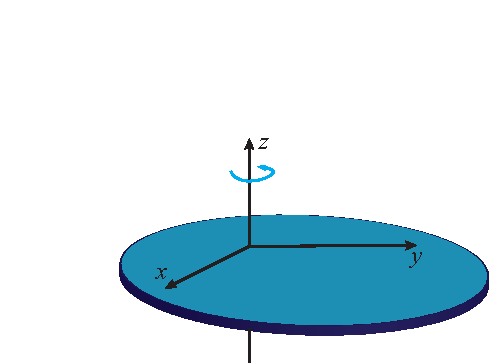
\includegraphics[scale=1.2]{C5-fig1.pdf}
	\caption{薄板垂直轴定理示意图}
	\label{C5-fig1}
\end{figure}

\section{绕定轴转动刚体的动能 \quad 动能定理} \label{5.3}

\begin{enumerate}
	
	\item 绕定轴转动刚体的动能
	
	\begin{equation}
		E = \dfrac{1}{2} J_z \omega^2 \label{C5-eq13}
	\end{equation}
	
	\item 力矩的功
	
	\begin{equation}
		A = \int_{\theta_1}^{\theta_2} M_z(\va*{F}) \dd{\theta} \label{C5-eq14}
	\end{equation}
	
	\item 绕定轴转动刚体的动能定理
	
	\begin{equation}
		\dd{\qty(\dfrac{1}{2} J_z \omega^2)} = \dd{A} \Longrightarrow \dfrac{1}{2} J_z \omega_2^2 - \dfrac{1}{2} J_z \omega_1^2 = A \label{C5-eq15}
	\end{equation}
	
\end{enumerate}

\newpage

\section{动量矩和动量矩守恒定律} \label{5.4}

\subsection{动量矩(角动量)}

\begin{definition}[动量矩(角动量)] \label{C5-df3}
	
	质点动量对$O$点之矩定义为位矢$\va*{r}$和动量$m\va*{v}$的叉积, 即
	
	\begin{equation}
		\va*{L}_O = \va*{r} \times m \va*{v} \label{C5-eq16}
	\end{equation}
	
	刚体对$z$轴的动量矩
	
	\begin{equation}
		L_z = J_z \omega \label{C5-eq17}
	\end{equation}
	
\end{definition}

\subsection{质点动量矩定理和动量矩守恒定律}

\begin{theorem}[质点动量矩定理] \label{C5-th3}
	在惯性系中, 质点对任意固定点$O$的动量矩对时间的导数, 等于作用在质点上所有力的合力对同一点$O$之矩. 
	
	\begin{equation}
		\dv{\va*{L}_O}{t} = \va*{r} \times \va*{F} = \va*{M}_O \label{C5-eq18}
	\end{equation}

\end{theorem}

\begin{axiom}[质点动量矩守恒定律] \label{C5-ax1}
	
	当作用在质点上的合力对固定点之矩总是为0时, 质点动量对该点的矩为常矢量. 
	
	\begin{equation}
		\va*{M}_O = 0 \Longrightarrow \va*{L}_O = \overrightarrow{\text{Const}} \label{C5-eq19}
	\end{equation}
		
\end{axiom}

\textbf{质点在有心力作用下的运动过程中, 质点对力心的动量矩守恒. }

\subsection{刚体绕定轴转动情况下的动量矩定理和动量矩守恒定律}

\begin{theorem}[刚体绕定轴转动情况下的动量矩定理] \label{C5-th4}
	\begin{equation}
		\dv{t}(J_z\omega) = M_z \label{C5-eq20}
	\end{equation}
	
	上式表明, 绕定轴转动刚体动量矩对时间的导数, 等于作用在刚体上所有外力对转轴之矩的代数和. 
	
	对式(\ref{C5-eq20})积分, 得
	
	\begin{equation}
		{(J_z\omega)}_t - {(J_z\omega)}_{t_0} = \int_{t_0}^{t} M_z \dd{t} \label{C5-eq21}
	\end{equation}

    上式表明, 定轴转动刚体的动量矩在某一时间间隔内的增量, 等于同一时间间隔内作用在刚体上的冲量矩. 
    
\end{theorem}

类似定律\ref{C5-ax1}, 有

\begin{equation}
	M_z = 0 \Longrightarrow J_z \omega = \overrightarrow{\text{Const}} \label{C5-eq22}
\end{equation}

\section{第4次作业部分题目归纳} \label{5.5}

\subsection{转动惯量的计算}

\begin{enumerate}
	
	\item (作业T5) 一块质量分布均匀的等边三角形薄板, 质量为$m$, 边长为$a$, 则它相对于通过其一边的轴的转动惯量为 \uline{$ma^2/8$}. 
	
\end{enumerate}

\subsection{圆盘(滑轮)}

\begin{enumerate}
	
	\item (作业T22) 一具有光滑转轴的定滑轮, 半径为$R$, 质量为$m/4$, 质量均匀分布在滑轮的边缘上, 从而对转轴的转动惯量为$J = mR^2/4$. 一轻绳跨过该定滑轮, 轻绳与滑轮间无相对滑动, 其左端有一质量为$m$的人爬在轻绳上, 而右端则系了一质量为$m/2$的重物, 如图(\ref{C5-fig2})所示. 当人从静止开始相对于轻绳匀速向上攀爬时, 求重物上升的加速度. 
	
\end{enumerate}

\begin{figure}[htbp]
	\centering
	\begin{minipage}[t]{0.48\textwidth}
		\centering
		\includegraphics[scale=0.6]{C5-fig2.eps}
		\caption{作业T22题图}
		\label{C5-fig2}
	\end{minipage}
	\begin{minipage}[t]{0.48\textwidth}
		\centering
		\includegraphics[scale=0.9]{C5-fig3.eps}
		\caption{作业T15题图}
		\label{C5-fig3}
	\end{minipage}
\end{figure}

\subsection{杆}

\begin{enumerate}
	
	\item (作业T15) 如图(\ref{C5-fig3})所示, 长为$l$, 质量为$M$的匀质直杆可绕过其一端$O$的水平位置无初速释放, 当转动到与水平方向成$30^{\circ}$时, 有一质量为$m = M/3$的子弹以水平速度$v_0$射入直杆的下端点并马上嵌在杆中不动, 则子弹射入后瞬间杆的角速度 \uline{$\omega = \sqrt{3g/8l} + v_0/4l$}.
	
\end{enumerate}


\chapter{狭义相对论力学基础}

\begin{introduction}
    \item \nameref{6.1}
    \item \nameref{6.2}
    \item \nameref{6.3}
\end{introduction}

\section{伽利略变换}\label{6.1}

实际上, 因为生活经验的关系, 我们都认识到公交车上的人的绝对速度$\va*{v}_a$等于车的速度$\va*{v}_e$和人相对于车的速度 $\va*{v}_r$的矢量和, 即

\begin{equation}
	\va*{v}_a = \va*{v}_e + \va*{v}_r \label{C6-eq1}
\end{equation}

其中, $\va*{v}_a$是人相对某一定系(如地面)的速度, $\va*{v}_r$是人相对于车的速度, $\va*{v}_e$是车相对于地面的速度. 

\subsection{伽利略变换的描述方法}

\begin{figure}[htbp]
	\centering
	\includegraphics[scale=0.9]{C6-fig1.eps}
	\caption{伽利略坐标变换示意}
	\label{C6-fig1}
\end{figure}

先建立两个惯性系$S$, $S'$, 且$S'$相对$S$沿$S$的$x$轴正向有速度$\va*{u}$, 以$S'$系和$S'$系原点重合时作为计时起点, 即$t = t' = 0$, 那么对于空间中一点$P$有

\begin{equation}
	\va*{r} = \va*{r}' + \va*{u}t \label{C6-eq2}
\end{equation}

分量式为

\begin{equation}
	\begin{cases}
		t' = t \\
		x' = x - ut \\
		y' = y \\
		z' = z
	\end{cases}
    \label{C6-eq3}
\end{equation}


将式(\ref{C6-eq3})称为\textbf{伽利略逆变换}, 正变换即是把$x$写在左边, $x'$写在右边. 



\subsection{对伽利略变换的讨论(伽利略变换的绝对时空观)}

如果时间空间均匀, 绝对, 与参考系无关, 比如: 

\vskip 0.3cm

\begin{enumerate}
	
	\item 运动飞船中的人测一根铁棍的长度等于地面上的人测那根铁棍的长度.
	
	\item 飞船上的人看一场电影的他认为自己过去的时间应该等于地面上的人看飞船里播放的电影的他认为自己用的时间. 
	
\end{enumerate}

\vskip 0.3cm

那么伽利略变换的正确性是显然的. 因为上面这两个例子就是伽利略变换可直接推出的结果, 这种观点就称为\textbf{绝对时空观}. 

所以说\textbf{伽利略变换是与绝对时空观绑定的, 伽利略变换本身是绝对时空观的数学表达式. }

\vskip 0.3cm

归纳如下: 

\begin{figure}[htbp]
	\centering
	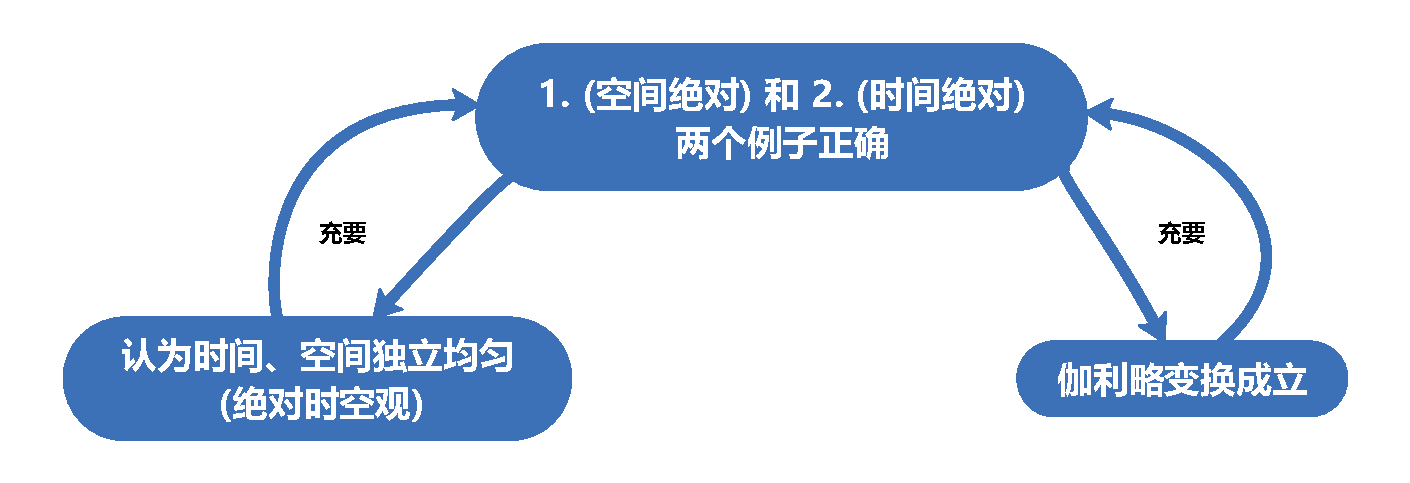
\includegraphics[scale=0.5]{C6-fig2.pdf}
	\caption{绝对时空观讨论}
	\label{C6-fig2}
\end{figure}

\subsection{伽利略相对性原理}

因为式(\ref{C6-eq3})中后三个坐标分量式恒成立, 又因为$\dd{t} = \dd{t'}$, 所以可得

\begin{equation}
	\begin{cases}
		\va*{v}'_x = \va*{v}_x - \va*{u} \\
		\va*{v}'_y = \va*{v}_y \\
		\va*{v}_z = \va*{v}_z
	\end{cases}
    \label{C6-eq4}
\end{equation}

再次求导可得

\begin{equation}
	\begin{cases}
		\va*{a}'_x = \va*{a}_x \\
		\va*{a}'_y = \va*{a}_y \\
		\va*{a}'_z = \va*{a}_z
	\end{cases}
    \label{C6-eq5}
\end{equation}

即速度和加速度的变换式. 显然\textbf{加速度有伽利略变换不变性. }

在$S$系与$S'$系分别用牛顿第二定律, 有

\begin{equation}
	\begin{cases}
		\va*{F} = m \va*{a} \\
		\va*{F}' = m' \va*{a}' 
	\end{cases}
    \label{C6-eq6}
\end{equation}

因为经典力学还认为质量是常量, 所以$\va*{F} = \va*{F}'$. 因此\textbf{牛顿定律有伽利略变换形式不变性}, 所以建立在牛顿定律上的经典力学均有伽利略变换形式不变性, 即\textbf{一切力学规律在所有惯性系中相同}(一切力学规律建立在牛顿定律上, 伽利略变换在两个惯性系间). 

\subsection{总结}

正像牛顿第二定律与动量定理, 冲量定理是相互可推证的一样, 伽利略变换本是自洽的经典力学的一块拼图, 但它却给后人留下了另一块空白. 至此, 其实只是交代的伽利略相对性原理, 也没有计算, 但这一部分对于整体理解经典力学和狭义相对论的关系有很重要的作用. 

\subsection{坏了}

先是麦克斯韦的电磁理论, 他理论推导出真空中光(电磁波)速为定值, 但因为速度无伽利略变换不变性, 这没法解释(大悲). 

然后物理学家就提出以太, 将以太作为一个绝对静止的参考系, 认为光速是相对于乙态系的. 

\begin{note}
	
	但其实这个时候就自相矛盾的, 伽利略相对性原理指出没有惯性系是特殊的, 现在人为建立了一个特殊惯性系. 
	
\end{note}

为了证明以太存在或者说光速也满足伽利略变换式, 迈克尔逊和莫雷做了以下实验: 

仪器相对地面静止, 以太绝对静止, 那么仪器相对以太有一个速度$\va*{v}$. 

\begin{figure}[htbp]
	\centering
	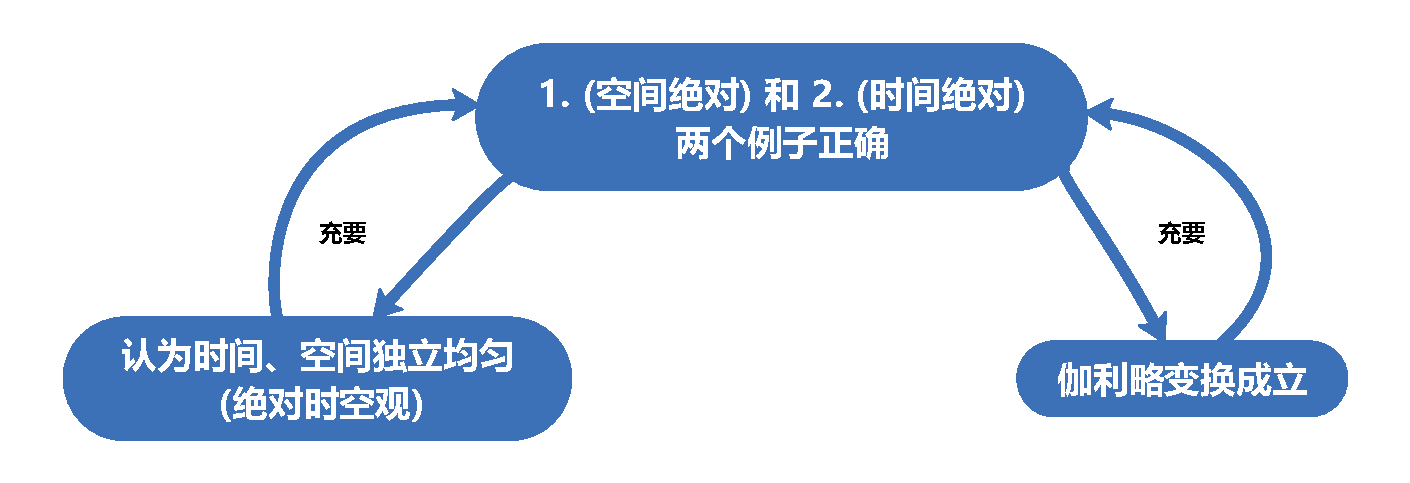
\includegraphics[scale=1.0]{C6-fig2.eps}
	\caption{迈克尔逊-莫雷实验示意}
\end{figure}

具体原理涉及到电磁波的干涉, 待各位大二上了解. 总之观察屏上应有干涉条纹且比较明显, 但结果是什么也没有, 所以经典理论遇到了困难. 

\newpage

\section{洛伦兹变换}\label{6.2}

\subsection{狭义相对论的两条基本假设}

为解决电磁学(光速$c$为定值)与经典力学(伽利略变换)间的矛盾, 爱因斯坦提出了狭义相对论的两条基本假设: 

\begin{postulate}[狭义相对论基本假设] \label{C6-po1}
	\begin{enumerate}
		
		\item 惯性系中物理定律相同(推广了伽利略的相对性原理); \label{C6-po1.1}
		
		\item 光速不变(无论如何观察光, 其速度为定值). \label{C6-po1.2}
		
	\end{enumerate}
\end{postulate}

\subsection{洛伦兹变换}

基于爱因斯坦的两条假设(\ref{C6-po1}), 可推导新的坐标变换. 

设一事件在$S$, $S'$系观察坐标为$(x, y, z, t)$, $(x', y', z', t')$. 

首先由假设 \ref{C6-po1.1} 得: 如果一个物体在$S$中不受力, 做匀速直线运动, 那么因为物理定律相同, 在$S'$系中观察其仍不受力, 还是匀速直线运动, 这就必然要有$x' = k_2x + b_1$, $y' = k_2y + b_2$, 即线性变换. 

再由假设 \ref{C6-po1.2} 得: 无论在$S$系还是$S'$系, 看一束光, 光的速度均应相同. 

最后, 因为伽利略变换的低速正确性, 这个新变换式在$\abs{\va*{u}} \ll c$时应能退化成伽利略变换. 

基于以上结论, 不妨写出以下变换式

\begin{equation}
	\begin{cases}
		x = k(x' + ut') \\
		x' = k'(x - ut)
	\end{cases}
    \label{C6-eq7}
\end{equation}

由于假设\ref{C6-po1.1}, 有$k' = k$. 将(\ref{C6-eq7})中两式相乘, 得

\begin{equation}
	xx' = k^2 (x' + ut') (x - ut) \label{C6-eq8}
\end{equation}

因为光速不变性, 我们把这个事件特殊化, 取为一束光运动到的坐标. 把$t = t' = 0$的时刻取为两惯性系重合且光从$x = x' = 0$位置射出那一刻, 那么有

\begin{equation}
	\begin{cases}
		x = ct \\
		x' = ct'
	\end{cases}
    \label{C6-eq9}
\end{equation}

代入式(\ref{C6-eq8}), 得

\begin{equation}
	k = \dfrac{c}{\sqrt{c^2 - u^2}} = \dfrac{1}{\sqrt{1 - \dfrac{u^2}{c^2}}} \label{C6-eq10}
\end{equation}

\newpage

于是

\begin{equation}
	\begin{cases}
		x = \dfrac{x' + ut'}{\sqrt{1 - \dfrac{u^2}{c^2}}} \\ \vspace{1ex}
		x' = \dfrac{x - ut}{\sqrt{1 - \dfrac{u^2}{c^2}}}
	\end{cases}
    \label{C6-eq11}
\end{equation}

两式消去$x$, $x'$分别得

\begin{equation}
	\begin{cases}
		t = \dfrac{t' + \dfrac{u x'}{c^2}}{\sqrt{1 - \dfrac{u^2}{c^2}}} \\ \vspace{2.0ex}
		t' = \dfrac{t - \dfrac{u x}{c^2}}{\sqrt{1 - \dfrac{u^2}{c^2}}}
	\end{cases}
    \label{C6-eq12}
\end{equation}

式(\ref{C6-eq11}), (\ref{C6-eq12})即为\textbf{洛伦兹变换式}, 其中用$S'$坐标描述$S$坐标的为逆变换, 反之则为正变换\footnote{正逆变换无绝对, 两者可以变换叫法. }. 

此外介绍洛伦兹速度变换: 

在$S$系, 有

\begin{equation}
	\begin{cases}
		v_x = \dfrac{\dd{x}}{\dd{t}} \\ 
		\vspace{1ex}
		v_y = \dfrac{\dd{y}}{\dd{t}} \\ \vspace{1ex}
		v_z = \dfrac{\dd{z}}{\dd{t}} 
	\end{cases}
    \label{C6-eq13}
\end{equation}

在$S'$系, 有

\begin{equation}
	\begin{cases}
		v_x' = \dfrac{\dd{x'}}{\dd{t'}} \\ 
		\vspace{1ex}
		v_y' = \dfrac{\dd{y'}}{\dd{t'}} \\ \vspace{1ex}
		v_z' = \dfrac{\dd{z'}}{\dd{t'}} 
	\end{cases}
	\label{C6-eq14}
\end{equation}

联立即得$v_x'$

\begin{equation}
	v_x' = \dfrac{\dd{x'}}{\dd{t'}} = \dfrac{\dfrac{\dd{x'}}{\dd{t}}}{\dfrac{\dd{t'}}{\dd{t}}} = \dfrac{\dfrac{x}{t} - u}{1 - \dfrac{u}{c^2} \dfrac{\dd{x}}{\dd{t}}} = \dfrac{v_x - u}{1 - \dfrac{u v_x}{c^2}} \label{C6-eq15}
\end{equation}

$v_y'$, $v_z'$同理. 

\newpage

\begin{note}
	一个记忆小技巧, 只记忆$x$和$t$的变换式, 要使用速度变换式时如此做: 
	
	\begin{equation*}
		v_x = \dfrac{x - ut}{\sqrt{1 - \dfrac{u^2}{c^2}}} / \dfrac{t - \dfrac{x c}{c^2}}{\sqrt{1 - \dfrac{u^2}{c^2}}}
	\end{equation*}
	
	两边同时除以$t$即可得到式(\ref{C6-eq15})的最后结果. 
	
\end{note}

\subsection{对于洛伦兹变换的讨论}

\begin{enumerate}
	
	\item 首先当然是要记清公式形式, 这个公式是这一部分的基础, 必须牢记. 
	
	\item 公式是在$S'$系相对$S$系有沿$x$轴正向大小为$u$的速度时推出的, 假若$S'$系相对$S$系向$x$轴负向有$u$速度, 分子上第二部分符号要取反. 同时也可能是$y$, $z$轴方向有相对速度, 要看清题意, 有相对速度的方向的速度变换式与无相对速度方向的速度变换式不同. 
	
	\item 讨论$x_1' - x_2'$的时候, 用$\frac{x_1 - ut_1}{\sqrt{1 - \frac{u^2}{c^2}}} - \frac{x_2 - ut_2}{\sqrt{1 - \frac{u^2}{c^2}}}$即可. 
	
\end{enumerate}

\vskip 0.4cm

\begin{example}
	地球上一人以10 s跑完100 m, 在速度为$0.98 c$的飞船中观察, 其用了多少时间, 跑了多远? 
	
	\begin{solution}
		
		参考图(\ref{C6-fig1}), 本题中, 将地球作为$S$系, 将飞船作为$S'$系. 
		
		本质上是已知$t_2 - t_1$, $x_2 - x_1$, 求$t_2' - t_1'$以及$x_2' - x_1'$.
		
		由于
		
		\begin{equation*}
			t_2' - t_1' = \dfrac{t_1 - \dfrac{u x_1}{c^2} - t_2 + \dfrac{u x_2}{c^2}}{\sqrt{1 - \qty(\dfrac{u}{c})^2}}
		\end{equation*}
		
		代入数据, 解得$t_2' - t_1' = 50.25$ s.
		
		同理可以求得$x_2' - x_1'$. 
		
	\end{solution}
	
\end{example}

\begin{example}
	地面上测到两飞船分别以$0.9c$, $-0.9c$的速度向相反方向飞行, 求一飞船相对另一飞船的速度. 
	
	\begin{solution}
		
		记向左飞的为\textcircled{1}, 向右飞的为\textcircled{2}.
		
		题目问的是在相对\textcircled{1}静止的参考系中观察\textcircled{2}的速度的大小, 不妨设相对\textcircled{1}和地球静止的系分别为$S$系和$S'$系, 在$S'$系, 即地球上观察\textcircled{2}的速度$v_x' = 0.9c$, 现在要求$v_x$.
		
		\begin{equation*}
			v_x = \dfrac{v_x' + u}{1 + \dfrac{u v_x'}{c^2}} = \dfrac{0.9c + 0.9c}{1 + 0.81} = 0.994c
		\end{equation*}
		
	\end{solution}
	
	\begin{note}
		
		本题有两个重点: 
		
		\begin{enumerate}
			
			\item 在理解$S$系, $S'$系和物体方面, 显然这是三个物体(系可以固连在物体上随物体运动), 因此要想套公式, 首先要分清哪个是$S$系, $S'$系和待研究物体. 
			
			\item 在一个系中观察物体, 其速度一定小于$c$, 但在一个系中观察两个物体, 他们的相对速度可以超过$c$. 
			
		\end{enumerate}
		
	\end{note}
	
\end{example}

\subsection{洛伦兹变换的意义}

$\bullet$ 揭示了空间, 时间, 物质运动间的联系. 

$\bullet$ 光速是一切运动速度的上限. 

\section{狭义相对论基础}\label{6.3}

\subsection{狭义相对论的时空观}

\subsubsection{同时性的相对性}

我们依然假设$S$, $S'$系是两个惯性系, $S'$系相对$S$系有沿$x$正方向的速度$\va*{u}$. 在$S$系测得事件1, 2的坐标为$\qty(x_1, y_1, z_1, t_1)$, $\qty(x_2, y_2, z_2, t_2)$; $S'$系测得事件1, 2坐标为$\qty(x_1', y_1', z_1', t_1')$, $\qty(x_2', y_2', z_2', t_2')$.

根据$S$系中观察的结论讨论: 

\begin{enumerate}
	
	\item $t_2 - t_1 = \Delta t = 0$, 则
	
	\begin{equation}
		t_2' - t_1' = \dfrac{\Delta t - \dfrac{u x_1}{c^2} + \dfrac{u x_2}{c^2}}{\sqrt{1 - \dfrac{u^2}{c^2}}} = \dfrac{u(x_2 - x_1)}{c^2\sqrt{1 - \dfrac{u^2}{c^2}}}
		\label{C6-eq16}
	\end{equation}
	
	若$x_2 = x_1$, 则有$t_2' - t_1' = 0$. 反之不一定, 且先后不确定. 
	
	\item $t_2 - t_1 = \Delta t \neq 0$, 则
	
	\begin{equation}
		t_2' - t_1' = \dfrac{c^2(t_2 - t_1) + u(x_2 - x_1)}{c^2\sqrt{1 - \dfrac{u^2}{c^2}}} 
		\label{C6-eq17}
	\end{equation}
	
	$t_2 - t_1$与$\frac{u(x_2 - x_1)}{c^2}$的大小关系决定了在$S'$系观察两事件的先后.
	
\end{enumerate}

因此, 对于不相关事件1, 2, 两个惯性系分别观察他们发生的先后是不太能直接认为相关的, 即$t_2 > t_1$不能直接说明$t_2'$和$t_1$的关系. 但对于因果事件, 如射击与击中, 无论如何观察, 均是射击在前, 击中在后.

\begin{example}
	有一长为600 m的列车, 其速度为$0.4c$, 地面上观察者发现有两个闪电同时击中火车前后端. 此时车上乘客测定的时间间隔为多少? 哪一端先被击中? 
	
	\begin{solution}
		
		记$t_1$为地面观察闪电击中前端的时刻, $t_2$为地面观测闪电击中后端的时刻, $t_1'$, $t_2'$意义易知.
		\begin{align*}
			x_1' - x_2' &= 600 \\
			t_1' - t_2' &= \dfrac{t_1 - t_2 - \dfrac{u x_1}{c^2} + \dfrac{u x_2}{c^2}}{\sqrt{1-0.16}} \\
			x_1 - x_2 &= \dfrac{x_1' - x_2' + u\qty(t_1' - t_2')}{\sqrt{1 - 0.16}} \\
			t_2 - t_1 &= 0
		\end{align*}
		
		解得$t_1' - t_2' = -8 \times 10^{-7}$ s, 即闪电在车上乘客看来先击中前端, 早$8 \times 10^{-7}$ s. 
		
	\end{solution}
	
\end{example}

\subsubsection{钟慢效应与尺缩效应}

\noindent \textbf{钟慢效应}

原时: 把某一个惯性系中同一地点先后发生的两个事件的时间间隔称为原时. 即在同一个惯性系同一地点用一个钟测出的时间差. 

从前面狭义相对论的“同时”的相对性的讨论知有: 

\begin{equation}
	t_2' - t_1' = \dfrac{t_2 - t_1 - \dfrac{u}{c^2} \qty(x_2 - x_1)}{\sqrt{1 - \dfrac{u^2}{c^2}}} \label{C6-eq18}
\end{equation}

由于$x_2 - x_1 = 0$, 则$t_2' - t_1' = \dfrac{\qty(t_2 - t_1)}{\sqrt{1 - \dfrac{u^2}{c^2}}} > t_2 - t_1$. 

所以说在$S'$系观察$S$系中先后发生的两件事比在S系观察先后发生的两件事用时长. 也就是一开始的例子, 在飞船中看一场电影的时间与地面上的人看飞船里这场电影时间是不同的. 

总结为: \textbf{原时最短, 任何惯性系中的观察者看别的惯性系的时间总会比本惯性系的时间慢}(相对自己静止的钟走1分, 相对自己运动的钟走1秒). 

\vskip 0.3cm

\begin{example}
    粒子寿命问题: 带静电的$\Pi$介子不稳定, 其静止寿命为$2.38 \times 10^{-8}$ s, 实验室测得一束$\Pi$介子速率为$0.99c$, 用狭义相对论计算实验人员观测出的$\Pi$介子寿命. 
	
	\begin{solution}
		\begin{equation*}
			t = \dfrac{t'}{\sqrt{1 - \dfrac{u^2}{c^2}}} = 1.772 \times 10^{-7} \textrm{~s}
		\end{equation*}
	\end{solution}
	
\end{example}

\begin{note}
	
	$t' = 2.38 \times 10^{-8}$ s是相对$\Pi$介子静止的惯性系的观测结果, 是原时
\end{note}

\vskip 0.3cm

\noindent \textbf{尺缩效应}

固有长度: 在相对被测物体静止的系中任意方式(无论是否同时)测得其首尾坐标并作差后得到的被测物体长度. 

在相对杆不静止的另一个惯性系中测量被测物体长度, 要求同时测得首尾端坐标并作差, 接下来取$S'$系相对$S$系$x$轴正向速度为$\va*{u}$, $S'$系相对被测物体静止. 

由于

\begin{align}
	x_2' - x_1' &= \dfrac{\qty(x_2 - x_1) - u\qty(t_2 - t_1)}{\sqrt{1 - \qty(\dfrac{u}{c})^2}} \label{C6-eq19} \\
	t_2 &= t_1 \label{C6-eq20}
\end{align}

所以

\begin{equation}
	x_2' - x_1' = \dfrac{x_2 - x_1}{\sqrt{1 - \qty(\dfrac{u}{c})^2}} > x_2 - x_1 \label{C6-eq21}
\end{equation}

其中, $x_2' - x_1'$为固有长度. 也就是说, 飞船中测物体长为1 m,地面上的人测飞船中这个物体长小于1 m. 

总结为: \textbf{原长最长, 沿相对运动方向的物体尺寸会收缩}. 如以下两例: 

\begin{figure}[H]
	\centering
	\begin{minipage}[t]{0.48\textwidth}
		\centering
		\includegraphics[scale=0.7]{C6-fig3.eps}
		\label{C6-fig3}
	\end{minipage}
	\begin{minipage}[t]{0.48\textwidth}
		\centering
		\includegraphics[scale=0.7]{C6-fig4.eps}
		\label{C6-fig4}
	\end{minipage}
\end{figure}

上右图中的$u$满足

\begin{equation*}
	\sqrt{3} S \sqrt{1 - \qty(\dfrac{u}{c})^2} = S \Rightarrow u = \dfrac{2\sqrt{3}c}{3}
\end{equation*}

\subsection{狭义相对论动力学基础}

传统的经典力学不满足洛伦兹变换, 所以要改造它, 建立相对论力学. 具体要重新定义质量、动量、能量, 使它们相应的守恒定律仍成立. 

\subsubsection{质速关系}

经典力学中有

\begin{equation}
	\va*{F} = m \va*{a} \label{C6-eq22}
\end{equation}

依照此式, $m$若不随$\va*{v}$变化, 那么只要时间足够长, 任何物体均可超越光速, 这与洛伦兹变换矛盾. 因此, 狭义相对论中给出质速关系

\begin{equation}
	m = \dfrac{m_0}{\sqrt{1 - \qty(\dfrac{u}{c})^2} \label{C6-eq23}}
\end{equation}

其中, $m_0$为本征质量(相对$m_0$静止的惯性系中测得的质量), $m$则为相对速度为$\va*{u}$的惯性系中测量得到的物体质量. 

由此得光子静止质量为0, 一切静止质量不为0的粒子速度必须小于$c$. 

进一步, 得到相对论动量和相对论动力学方程

\begin{align}
	\va*{p} &= m \va*{v} = \dfrac{m_0}{\sqrt{1 - \qty(\dfrac{u}{c})^2}} \va*{v} \label{C6-eq24} \\
	\va*{F} &= \dv{\va*{p}}{t} = \dv{t}(\dfrac{m_0}{\sqrt{1 - \qty(\dfrac{u}{c})^2}} \va*{v}) \label{C6-eq25}
\end{align}

\subsubsection{质能方程}

\begin{equation}
	E = mc^2 = \dfrac{m_0}{\sqrt{1 - \qty(\dfrac{u}{c})^2}} c^2 = m_0 c^2 + E_{\textrm{k}} = E_0 + E_{\textrm{k}} \label{C6-eq26}
\end{equation}

物体质量由动能和静止能量构成, 注意此时$E_{\textrm{k}}$不能写成$\dfrac{1}{2}mv^2$的形式. 

\vskip 0.3cm

\begin{example}
	两个静止质量$m_0$的粒子, 一个$v=0$, 另一个$v=0.6c$, 它们对心碰撞后粘在一起, 求复合粒子的静止质量. 
	\begin{solution}
		
		设合并后速度为$v'$, 静止质量为$m'$. 
		\begin{align}
			\text{动量守恒:~} \dfrac{m_0}{\sqrt{1-{(0.6)^2}}} v &= \dfrac{m'}{\sqrt{1-\dfrac{{v^2}'}{{c^2}}}} v' \label{C6-eq27} \\
			\text{能量守恒:~} m_0 {c^2} + \dfrac{m_0}{\sqrt{1-{(0.6)^2}}} {c^2} &= \dfrac{m'}{\sqrt{1 - \dfrac{{v^2}'}{{c^2}}}} {c^2} \label{C6-eq28}
		\end{align}
		
		式(\ref{C6-eq28})中消去$c^2$, 将式(\ref{C6-eq27})中$m'$用$v'$表示代入式(\ref{C6-eq28})得$v'$, 代入式(\ref{C6-eq27})得$m'$. 
		
	\end{solution}
	
\end{example}

\begin{center}
	\textcolor[RGB]{18,29,57}{\textbf{小结}}
\end{center}

本章从经典力学中的伽利略变换讲起, 说明了他与经典力学时空观的紧密联系, 再从实际实验中无法解释的现象说起, 提出狭义相对论, 并用狭义相对论创建了一套新的时空观, 一套新的动力学、能量方程. 
本章启发性很强, 题目在弄明白公式后难度不大, 本章中一些知识点在诸如《星际穿越》等科幻电影中时有出现, 对大家欣赏艺术也有帮助. 



\chapter{电场}

\begin{introduction}
	\item \nameref{7.1}
	\item \nameref{7.2}
	\item \nameref{7.3}
	\item \nameref{7.4}
	\item \nameref{7.5}
\end{introduction}

电荷运动时同时激发电场与磁场, 相互联系, 较难研究, 本章在电荷静止的条件下研究其激发的电场. 正像研究牛顿定律离不开刚体, 质点, 速度, 加速度, 研究电场也离不开电荷量, 导体, 库仑定律, 场强等模型或物理量. 

\section{与电场有关的概念}\label{7.1}

\begin{definition}[电荷量]
	电中性物体得失正负电荷时会成为带电体, 其显露的电荷数为其电荷量. 
\end{definition}

\begin{axiom}[电荷守恒]
	宏观过程中, 一种电荷消失或出现, 一定有等量异种电荷消失或出现. 
	
	此时电荷守恒表述为: 电荷既不能被创造也不能被消灭, 只能从一部分转移到另一部分. 微观过程中, 电子可以由“无”到“有”, 从“有”至“无”, 如光子与原子核作用有
	
	\begin{align*}
		&r \rightarrow e^{+} + e^{-} \quad \text{(电子创生)} \\
		&e^{+} + e^{-} \rightarrow r \quad \text{(电子湮没)}
	\end{align*}
	
	但系统总电荷守恒. 
	
	因此无论宏观微观电荷守恒可表述为系统总电荷守恒, 在计算静平衡时可作为一个方程式用. 
\end{axiom}

\begin{axiom}[库仑定律]
	真空中, 两个静止点电荷之间的作用力$\va*{F}_{12}(\va*{F}_{21})$满足: 
	
	\begin{equation}
		\abs{\va*{F}_{12}} = k \dfrac{q_1 q_2}{r^2} \label{C7-eq1}
	\end{equation}
	
	方向沿两点电荷连线, 同性相斥, 异性相吸. 
	
	\vskip 0.2cm
	
	其中, $k = \dfrac{1}{4\pi \varepsilon_0}$, 为了后续推导方便, 注意用$\dfrac{1}{4\pi \varepsilon_0}$代替$k$, 戒除高中的习惯. 
	
\end{axiom}

\begin{figure}[H]
	\centering
	\includegraphics[scale=1.0]{C7-fig1.eps}
	\caption{两点电荷间的作用}
	\label{C7-fig1}
\end{figure}

\begin{note}
	
	$\bullet$ 点电荷为理想模型, 当两带电体自身线度与之间距离相比可忽略时可自然等效. 
	
	$\bullet$ 真空中$\varepsilon=\varepsilon_0$, 而在均匀介质中$\varepsilon=\varepsilon_0\varepsilon_r$, 代入公式时要注意($\varepsilon_0$为真空中介电常数, $\varepsilon$为某均匀同性介质中的介电常数, $\varepsilon_r$则为该介质的相对介电常数, 无单位). 
	
	$\bullet$ 若有许多点电荷, 则任一点电荷所受库仑力为其他点电荷的力的矢量和. 
	
\end{note}

\begin{definition}[电场]
	万有引力不是一种接触力, 两块磁石之间不用接触也可有里的作用, 力如何传递呢? 因为超距作用被否认了, 所以提出了场. 力由场传递, 而场由带电体激发, 静电场是相对观察者静止的电荷激发出的电场. 场是一种物质, 电荷激发出了这种物质, 电荷在场中受场的力, 运动时还会接受场做的功, 为了描述场(就像描述宏观物体所提出质量, 速度一样)提出场的强度(重力加速度就可以理解为重力场的场强). 
\end{definition}

\begin{definition}[电场强度]
	
	\begin{equation}
		\va*{E} = \dfrac{\va*{F}}{q_0} \label{C7-eq2}
	\end{equation}
	
	电场强度是电场本身的性质, 与电场中是否存在实验电荷无关. 就像一个六十公斤的人无论是否去称体重均为六十公斤一样. 
	
	$\bullet$ 特别地, 点电荷场强由$q_1$激发
	
	\begin{equation}
		E = \dfrac{q_1}{4 \pi \varepsilon_0 r^2} \label{C7-eq3}
	\end{equation}
	
	$\bullet$ 点电荷系场强由点电荷$\va*{E}$矢量叠加得到. 
	
	$\bullet$ 连续带电体场强, 取微元, 对任一微元列出场强表达式, 再进行矢量积分即可(把矢量分解成$\va*{x}$, $\va*{y}$方向的分量后与一维线积分一样, 偶尔可用矢量对称性简化过程). 
	
\end{definition}

下面对几种常见连续带电体进行求解. 

\vskip 0.3cm

\begin{example}
	有限长均匀带电细棒, 电荷线密度为$\lambda$, 求距棒$a$处一点$P$的场强.
	
	\begin{figure}[H]
		\centering
		\includegraphics[scale=1.0]{C7-fig2.eps}
		\caption{有限长均匀带电细棒}
		\label{C7-fig2}
	\end{figure}
	
	\begin{solution}
		假设细棒带正电, 带负电可把$\lambda$变为负值代入以调整方向. 
		
		由点电荷的场强公式有
		
		\begin{equation*}
			\begin{cases}
				E = \dfrac{1}{4\pi \varepsilon_0} \dfrac{\lambda \dd{y}}{r^2} \\
				r \sin \theta = a 
			\end{cases}
		\end{equation*}
		
		于是
		
		\begin{align*}
			E &= \dfrac{\sin^2 \theta}{4\pi \varepsilon_0} \dfrac{\lambda \dd{y}}{a^2} \\
			E_x &= \dfrac{\sin^3 \theta}{4\pi \varepsilon_0} \dfrac{\lambda \dd{y}}{a^2} \\
			E_y &= \dfrac{\sin \theta \cos \theta}{4\pi \varepsilon_0} \dfrac{\lambda \dd{y}}{a^2} 
		\end{align*}
		
		又\footnote{这里微元为$\dd{y}$, 但明显要对$\theta$进行积分, 所以要找$\dd{y}$与$\theta$的关系, 这种变换积分未知量的操作在日后习题考试中常有. }
		
		\begin{equation*}
			- \dfrac{a}{\tan \theta} = y ~\Rightarrow~ \dd{y} = a \csc^2 \theta \dd{\theta}
		\end{equation*}
		
		如此便得到
		
		\begin{align*}
			E_x &= \int_{\theta_1}^{\theta_2} \dfrac{\lambda}{4 \pi \varepsilon_0 a} \sin \theta \dd{\theta} = \dfrac{\lambda}{4 \pi \varepsilon_0 a} (\cos \theta_1 - \cos \theta_2) \\
			E_y &= \int_{\theta_1}^{\theta_2} \dfrac{\lambda}{4 \pi \varepsilon_0 a} \cos \theta \dd{\theta} = \dfrac{\lambda}{4 \pi \varepsilon_0 a} (\sin \theta_2 - \sin \theta_1)
		\end{align*}
		
	\end{solution}
	 
\end{example}

\begin{note}
	
	\indent 首先要记住$\dfrac{\lambda}{4\pi \varepsilon_0}$, 然后记住$E_x$与$\cos \theta$有关, $E_y$与$\sin \theta$有关. $\cos \theta_1$, $\cos \theta_2$的正负决定$E_x$是从棒指向$P$点还是从$P$点指向棒. 如果棒带正电自然为前者, 反之把$\lambda$换成负的即可(但形式不变, 所以可以统一用正电记). $y$方向就看$P$点离哪一端近, 这样哪一边的$y$方向合场强小, 电场就向哪一边, 如下图所示. 
	
	\begin{figure}[h]
		\centering
		\includegraphics[scale=0.8]{C7-fig3.eps}
		\label{C7-fig3}
	\end{figure}
	
	均匀带电的话两端的$l$的$y$方向的场强相抵, 则$P$点在$y$方向上的场强向下, 大小为$E_y = \dfrac{\lambda (\sin \theta_2 - \sin \theta_1)}{4 \pi \varepsilon_0 a}$. 
	
\end{note}

\vskip 0.3cm

\begin{example}
	无限长均匀带点棒, 此时认为$\theta_1=0$, $\theta_2=\pi$, $P$点无论在何处, 均相当于中点位置, 于是$E_y=0$, $E_x$由前推导知为$\dfrac{\lambda}{2 \pi \varepsilon_0 a}$. 
\end{example}

\vskip 0.3cm

\begin{example}
	对于均匀带电细圆环轴线上的场强分布, 首先就要想到除$x$方向外所有场强均相互抵消为0, 故合场强沿$x$方向, 取一小段$r\dd{\theta}\lambda$, 则其在$P$点$x$方向场强为
	\begin{align*}
		\dd{E_x} &= \dfrac{1}{4\pi\varepsilon_0} \dfrac{r\dd{\theta}\lambda}{a^2+r^2}\cos\varphi \\
		\cos \varphi &= \dfrac{a}{\sqrt{a^2+r^2}}
	\end{align*}
    
    \begin{figure}[h]
    	\centering
    	\includegraphics[scale=1.4]{C7-fig4.eps}
    	\caption{均匀带电细圆环}
    \end{figure}
    
    对$\theta$从0到$2\pi$积分即可得
	
	\begin{equation*}
		E_x=\dfrac{Qa}{4\pi\varepsilon_0{(a^2+r^2)}^{{\frac{3}{2}}}}
	\end{equation*}
    
    其中$Q=2\pi r\lambda$为总电量, 不用$\lambda$表示是为了方便下面的推导. 
	
\end{example}

\vskip 0.3cm

\begin{example}
	内外半径分别为$R_1$, $R_2$的圆环形平面均匀带电, 带电量$Q$, 轴线上的任一点的场强. 圆环形可以当作由无数细圆环拼成, 我们取一半径为$r$, 宽为$\dd{r}$的细圆环, 电荷面密度
	
	\begin{equation*}
		\sigma = \dfrac{Q}{\pi R_2^2 - \pi R_1^2}
	\end{equation*}
	
	\begin{figure}[h]
		\centering
		\includegraphics[scale=1.3]{C7-fig5.eps}
		\caption{均匀带电圆环平面}
	\end{figure}
	
	细圆环电量为$2\pi r_1 \sigma \dd{r}$, 由上例知这一个半径$r_1$的细圆环产生的电场强度为
	
	\begin{align*}
		E_0 &= \dfrac{Q_1 a}{4 \pi \varepsilon_0 {(a^2 + r_1^2)}^{{\frac{3}{2}}}} \\
		Q_1 &= \dfrac{2\pi r_1Q}{\pi R_2^2 - \pi R_1^2}
	\end{align*}
	
	从$R_1$到$R_2$对$\dd{r}$积分得
	
	\begin{equation*}
		E = \dfrac{\sigma x}{2 \varepsilon_0}\qty[\dfrac{1}{{(r_1^2 + x^2)}^{{\frac{1}{2}}}} - \dfrac{1}{{(r_2^2 + x^2)}^{{\frac{1}{2}}}}]
	\end{equation*}
	
\end{example}

\begin{note}
	
	$\bullet$ 如果是一个圆形平板, $R_1=0$. 
	
	$\bullet$ 如果$a\gg R_1$, $a\gg R_1$, 可看成电量为$Q$的点电荷, $E = \dfrac{Q}{4 \pi \varepsilon_0 a^2}$.
	
	$\bullet$ 若为无限大平板, $R_2 \rightarrow \infty$, $R_1=0$, $E = \dfrac{\sigma}{2\varepsilon_0}$.
	
	\vskip 0.2cm
	
	$\bullet$ 这一部分需要自己多推导几次, 防止遗忘. 
	
\end{note}

\section{描绘电场的方法} \label{7.2}

在上一节\nameref{7.1}中, 我们讨论了电场有关的物理量, 并推导了几种规则图形的场强分布, 以下要提出描绘电场的方法以及两个相关定理. 

\subsection{电场线}

用电场线描绘电场. 电场线上任一点的切线方向即为这一点场强的方向, 电场线的疏密反映出附件场强的大小. 

其实和高中课本上的没太大区别. 至于电场的提出的具体思路还是说不清, 只是知道它确实是有用即可. 

\begin{note}
	
	$\bullet$ 电场线起于正电荷或无穷远处, 终于负电荷或无穷远处. 
	
	$\bullet$ 电场线不相交, 不重合, 不闭合. 
	
\end{note}

\subsection{电通量}

电场中穿过任意曲面$S$的电场线数目, 用$\varPhi_e$表示. 具体来说$\varPhi_e = \va*{E} \cdot \va*{S}_{\bot} = E S \cos \theta$. 

\vskip 0.3cm

如果是一个曲面, 就要用三维面积分$\displaystyle \varPhi_e = \int_{S} {\va*{E} \cdot \dd{\va*{S}}}$. 

\vskip 0.3cm

规定闭合曲面电场线穿出为正方向, 穿出为负方向. 

\begin{figure}[h]
	\centering
	\includegraphics[scale=1.4]{C7-fig6.eps}
	\caption{电场线穿过曲面}
\end{figure}

\subsection{静电场高斯定理}

\begin{theorem}[静电场高斯定理]\label{C7-thgs}
	真空中任何静电场中, 穿过任一闭合曲线的电场强度通量, 数值上等于该闭合曲面包围电荷量的代数和乘$\dfrac{1}{\varepsilon_0}$, 即
	
	\begin{equation}
		\varPhi_e = \dfrac{1}{\varepsilon_0} \sum\limits_{S\text{内}} q_i \label{C7-eq4}
	\end{equation}
	
\end{theorem}

下面分几种情况证明其正确性. 

\begin{enumerate}
	\item 穿过包围点电荷$q$的任意闭合曲面$S$有
	
	\begin{equation}
		\varPhi_e = \dfrac{q}{\varepsilon_0} \label{C7-eq5}
	\end{equation}
	
	对于一个电荷量为$q$的点电荷, 其电场强度
	
	\begin{equation}
		\va*{E} = \dfrac{q}{4 \pi \varepsilon_0 r^2}\va*{e_r} \label{C7-eq6}
	\end{equation}
	
	若用一规则球壳包围它, 则
	
	\begin{equation}
		\varPhi_e = \int_{S}{\va*{E} \cdot \dd{\va*{S}}} = \dfrac{q \cdot 4 \pi r^2}{4 \pi \varepsilon_0 r^2} = \dfrac{q}{\varepsilon_0} \label{C7-eq7}
	\end{equation}
	
	这个球壳半径不影响结果, 用任意一个不规则曲面包围这个球壳也会有磁通量相同.
	
	\begin{figure}[h]
		\centering
		\includegraphics[scale=1.4]{C7-fig7.eps}
	\end{figure}
	
	\item 不包围电荷的高斯面的$\varPhi_e = 0$, 有多少电场线穿入就有多少电场线穿出, 故$\varPhi_e = 0$. 
	
	\vskip 0.3cm
	
	\item 详见课本P 253, $\displaystyle \oint_S E \cdot \dd{S} = \dfrac{1}{\varepsilon_0} \sum\limits_{i = 1} q_i$
	
\end{enumerate}

\begin{note}
	
	$\bullet$ 高斯定理中面元处的场强是该处的真实场强, 而非限定的其包围的电荷的场强. 
	
	$\bullet$ 高斯定理的有效应用还是有一定的限制, 实际上如果高斯面为不规则曲面, 使用高斯定理的意义不大. 其常用于求对称物体场强部分布. 
	
\end{note}

\newpage 

\begin{example}
	求均匀带正电球面内外场强, 球面电荷量为$Q$.
	
	\begin{figure}[h]
		\centering
		\includegraphics[scale=1.1]{C7-fig8.eps}
		\caption{均匀带正电球面}
	\end{figure}
	
	\begin{solution}
		设球面半径为$R$. 无论是球面内的$P_1$, 还是球面外的$P_2$, 均有场强方向沿着$\overrightarrow{OP_1}$或沿$\overrightarrow{OP_2}$方向, 所以作一半径为$r$的高斯球面, 其上任一点场强大小相同, 方向均沿半径方向, 所以
		
		\begin{align*}
			E &\perp S_{\bot} \\ 
			\varPhi_e &= 4 \pi r^2 E 
		\end{align*}
		
		对任意半径小于$R$的高斯球面均有
		
		\begin{equation*}
			\varPhi_e = \dfrac{1}{\varepsilon_0}\sum\limits_{i} q_i 
		\end{equation*}
	    
	    因为球面内无电荷, 所以电通量为0, 于是$E=0$, 球面内无电场分布. 
		
		当取高斯球面半径大于$R$时, 有$4\pi\varepsilon_0 r^2 E = Q$, 此时可得
		
		\begin{equation*}
			E = \dfrac{Q}{4\pi\varepsilon_0 r^2}
		\end{equation*}

		综上, 球面电场分布为
		
		\begin{equation*}
			E = \begin{cases}
				0, ~r &< R \\
				\dfrac{Q}{4\pi\varepsilon_0 r^2}, ~r &\geq R 
			\end{cases}
		\end{equation*}
		
		\begin{figure}[h]
			\centering
			\includegraphics[scale=1.2]{C7-fig9.eps}
			\caption{场强分布示意}
			\label{C7-fig9}
		\end{figure}
		
	\end{solution}
	
\end{example}

\begin{example}
	对于均匀带电球体, 其半径为$R$, 电荷量为$Q$, 求其场强分布. 
	
	\begin{figure}[h]
		\centering
		\includegraphics[scale=1.4]{C7-fig10.eps}
		\caption{均匀带电球体}
	\end{figure}
	
	\begin{solution}
		
		(1) 当高斯曲面选为半径小于$R$的均匀球面时有
		
		\begin{equation*}
			4\pi r_1^2 E = \dfrac{Q \cdot {{{\dfrac{4}{3}}\pi r_1^3}}}{{\dfrac{4}{3}}\pi R^3} = {\qty(\dfrac{r_1}{R})}^3 Q \Rightarrow E = \dfrac{Q r_1}{4\pi R^3} 
		\end{equation*}
	
	    (2) 当高斯曲面选为半径大于R的均匀球面时有
	    
	    \begin{equation*}
	    	4\pi r_2^2 E = \dfrac{Q}{\varepsilon_0} \Rightarrow E = \dfrac{Q}{4\pi\varepsilon_0 r_2^2}
	    \end{equation*}
	    
	    方向可由球体带电性质判断. 这个结果和地心引力以及重力加速度随离地心半径的关系一致. 
	    
	    \begin{figure}[h]
	    	\centering
	    	\includegraphics[scale=1.4]{C7-fig11.eps}
	    	\caption{场强分布示意}
	    \end{figure}
	    
	\end{solution}
	
\end{example}

\newpage

\begin{example}
	有一无限长均匀带电的圆柱面, 已知其横截面半径为$R$, 沿圆柱面轴线方向的电荷线密度为$\lambda$, 求圆柱面内外场强分布. 
	
	\begin{figure}[h]
		\centering
		\includegraphics[scale=0.8]{C7-fig12.eps}
		\caption{无限长均匀带电的圆柱面}
	\end{figure}
	
	\begin{solution}
		
		对于空间上任一点$P$, $P$点场强在不沿半径方向相互抵消, 故场强沿半径方向, 仍有$\va*{E}\perp \va*{S}_{\bot}$. 
		
		取高斯面形状为圆柱形, 因为圆柱面无限长, 在距离中心轴距离相同的位置上场强大小相等所以不用考虑场强在沿轴线的变化情况. 所以$h$不影响求解. 
		
		当$r \leq R$时, 有
		
		\begin{equation*}
			2 \pi r h E = q
		\end{equation*}
		
		因为圆柱面内无电荷, 所以$E = 0$.
		
		当$r > R$时, 有
		
		\begin{equation*}
			2 \pi r h E = \dfrac{h \lambda}{\varepsilon_0} \Rightarrow E = \dfrac{\lambda}{2 \varepsilon_0 \pi r}
		\end{equation*}
		
		这里圆柱上下底面$\va*{E}\cdot \va*{S}_{\bot} = 0$, 故只有侧面有电通量. 
		
		综上所述, 
		
		\begin{equation*}
			E = \begin{cases}
				0, r \leq R \\
				\dfrac{\lambda}{2 \varepsilon_0 \pi r}, r > R
			\end{cases}
		\end{equation*}
		
	\end{solution}
	
\end{example}

\begin{note}
	
	请依此法尝试求解无限长均匀带电圆柱的场强分布. 同样还是场强方向只沿半径方向, 高斯面仍可取圆柱面且上下底面均无电通量. 
	
\end{note}

\newpage

\begin{example}
	均匀带电的无限大平面薄板, 电荷面密度为$\sigma$, 求场强分布. 
	
	\begin{figure}[h]
		\centering
		\includegraphics[scale=0.7]{C7-fig13.eps}
		\caption{均匀带电的无限大平面薄板}
	\end{figure}
	
	\begin{solution}
		由对称性, 任意位置的$P$点均有场强方向垂直平面. 取高斯面如图. 
		
		同样因为是无限大平面, $r$的大小不影响$E$的结果. 
		
		于是有
		
		\begin{equation*}
			2 \pi r^2 E = \dfrac{\sigma S}{\varepsilon_0} \Rightarrow E = \dfrac{\sigma}{2\varepsilon_0}
		\end{equation*}
		
		注意到$E$只与$\sigma$有关, 与$P$点到$O$平面的垂直距离无关. 
		
	\end{solution}
	
\end{example}

\begin{note}
	
	这个模型有两种变形: 
	
	(1) 把“薄板”改为有厚度的导体板, 此时取高斯面要取成一个底面在导体板内, 一个底面在导体板外的形式. 这样因为导体内无电场, 于是有
	
	\begin{figure}[h]
		\centering
		\includegraphics[scale=0.6]{C7-fig14.eps}
	\end{figure}
	
	\begin{equation*}
		\pi r^2 E = \dfrac{\pi r^2 \sigma}{\varepsilon_0} \Rightarrow E = \dfrac{\sigma}{\varepsilon_0}
	\end{equation*}
	
	后面会知道导体内无电荷分布, 电荷集中在“表面”. 
	
	(2) 把“一个”变成“两个”, 且这两个薄板带电荷量相反, 即
	
	\begin{figure}[H]
		\centering
		\includegraphics[scale=0.6]{C7-fig15.eps}
	\end{figure}
	
	此时分两步取高斯面. 
	
	第一步, 取
	
	\begin{figure}[H]
		\centering
		\includegraphics[scale=0.7]{C7-fig16.eps}
	\end{figure}
	
	可得$E = 0$, 即两板外$E = 0$. 
	
	第二步, 取
	
	\begin{figure}[H]
		\centering
		\includegraphics[scale=0.7]{C7-fig17.eps}
	\end{figure}
	
	可得两板间$E = \dfrac{\sigma}{\varepsilon_0}$
	
	这在后面电容器中有些作用. 
\end{note}

\subsection{环路定理}

高斯定理说明电场为有源场, 安培环路定理说明电场为保守力场. 

\textbf{静电力做功的特点}

\begin{figure}[H]
	\centering
	\includegraphics[scale=0.7]{C7-fig18.eps}
	\caption{静电力做功示意}
\end{figure}

假设$O$点有一个元电荷激发的电场, 一试验电荷从$a$到$b$运动, 则

\begin{equation}
	\dd{A} = \va*{F} \cdot \dd{\va*{l}} = q_0 \va*{E} \cdot \dd{\va*{l}} =  \dfrac{q_0 q}{4 \pi \varepsilon_0 r^2}\va*{e_r} \cdot \dd{\va*{l}} = \dfrac{q_0 q}{4 \pi \varepsilon_0 r^2} \cos \theta \dd{l} = \dfrac{q_0 q}{4 \pi \varepsilon_0 r^2} \dd{r} \label{C7-eq8}
\end{equation}

则从$a$到$b$电场总功

\begin{equation}
	A = \int_{a}^{b} \dd{A} = \int_{r_a}^{r_b} {\dfrac{q_0 q}{4 \pi \varepsilon_0 r^2} \dd{r}} = \dfrac{q_0 q}{4 \pi \varepsilon_0 r^2}(\dfrac{1}{r_a} - \dfrac{1}{r_b}) \label{C7-eq9}
\end{equation}

即单个电荷激发出的电场做功只与试验电荷与中心电荷的距离有关, 而与路径无关. 静电场与重力场一样是保守场. 

\begin{theorem}[静电场的环路定理]
	试验电荷从$a$经闭合路径$l_1$, $l_2$回到$a$, 在这个过程中电场力所做的功为
	
	\begin{figure}[H]
		\centering
		\includegraphics[scale=1.0]{C7-fig19.eps}
	\end{figure}
	
	\begin{equation}
		A = \oint_{L}{q_0 E \cdot \dd{l}} = 0 \label{C7-eq10}
	\end{equation}
	
	静电场场强沿任何闭合路径的线积分为零. 
\end{theorem}

\subsection{电势与电势能}

前面讲到静电场为保守场, 即做功只与电荷始末位置有关, 因此可引入势能$E_{\textrm{p}a}$, 即

\begin{equation}
	E_{\textrm{p}b} - E_{\textrm{p}a} = \int_{a}^{b}{\va*{E} \cdot q \cdot \dd{\va*{l}}} \Rightarrow \dfrac{E_{\textrm{p}b} - E_{\textrm{p}a}}{q}  = \int_{a}^{b}{\va*{E} \cdot \dd{\va*{l}}} \label{C7-eq11}
\end{equation}

式(\ref{C7-eq11})右侧与$q$无关, 不包含任何试验电荷量, 因此是电场的性质, 与电场强度异曲同工, 而左侧是势能变化量除以试验电荷量, 定义为从$a$到$b$过程中的电势差$U_{ab}$, 其中$\dfrac{E_{\textrm{p}b}}{q}$定义为$b$处电势$V_b$, $\dfrac{E_{\textrm{p}a}}{q}$定义为$a$处电势$V_a$. 它们满足

\begin{equation}
	U_{ab} = V_b - V_a
\end{equation}

可与高度和高度差类比. 

\textbf{电势的求解}

\begin{enumerate}[itemindent=1em]
	
	\item 从前面以单个点电荷形成的电场为条件推出的电势表达式来看
	\begin{equation}
		V_a = \dfrac{q_0}{4 \pi \varepsilon_0} \dfrac{1}{r_a} \label{C7-eq12}
	\end{equation}
	那么当$r_a \rightarrow +\infty$时$V_a = 0$, $V_a$相当于$U_{a +\infty}$, 即\textbf{某试验电荷在某点的电势能为从该点将该试验电荷移到无穷远处(零势能点)过程中电场所做功的大小}, 电势自然为电势能除以试验电荷量. 
	
	因此在求电势的时候即可使用$U_{a +\infty}$的思路, 先求电势能除以试验电荷量, 一般要用到电势叠加原理(这个方法常用于带电圆环产生的电场的电势计算), 由前定义 
	
	\begin{equation}
		V_p = \int_{p}^{+\infty}{\va*{E}\cdot \dd{\va*{l}}} \label{C7-eq13}
	\end{equation}
	
	因为电场强度服从矢量加和, 即
	
	\begin{equation}
		V_p = \int_{p}^{+\infty}{(\va*{E}_1 + \va*{E}_2 + \cdots + \va*{E}_n)} \dd{\va*{l}} = V_{1p} + V_{2p} + \cdots + V_{Np} = \sum\limits_{i=1}^{n}{V_{ip}} \label{C7-eq14}
	\end{equation}
	
	即某位置的电势为该位置在每一个单独场源电荷形成的电场中的电势之和
	
	\begin{equation}
		V_p = \dfrac{1}{4\pi\varepsilon_0}\sum\limits_{i=1}^{n}\dfrac{q_i}{r_i}
	\end{equation}

	电势是标量, 因此在求电势的积分时不需分解, 比较方便. 
	
	\item 对于用积分不太方便, 比如均匀带电的球体就可先用高斯定理求出$\va*{E}$沿半径的分布, 再用
	
	\begin{equation*}
		V_p = \int_{p}^{+\infty}{\va*{E}\cdot \dd{\va*{l}}}
	\end{equation*}
	
	积分求解. 
	
\end{enumerate}

\begin{example}
	(应用方法一) 电荷密度$\lambda$均匀分布在半径为$R$的圆环上, 计算$P$点电势. 
	
	\begin{figure}[H]
		\centering
		\includegraphics[scale=1.2]{C7-fig20.eps}
		\caption{均匀带电细圆环}
	\end{figure}
	
	\begin{solution}
		
		取一段小圆弧, 其电量为$\lambda R \dd{\theta}$, 它在$P$点电势为
		
		\begin{equation*}
			\dfrac{1}{4\pi\varepsilon_0}\int\dfrac{\lambda R \dd{\theta}}{\sqrt{R^2 + a^2}}
		\end{equation*}
		
		由电势叠加
		
		\begin{equation*}
			V_p = \dfrac{\lambda R}{4\pi\varepsilon_0\sqrt{R^2+a^2}}\int_{0}^{2\pi}\dd{\theta} = \dfrac{2\pi\lambda R}{4\pi\varepsilon_0\sqrt{R^2+a^2}} = \dfrac{Q}{4\pi\varepsilon_0\sqrt{R^2+a^2}}
		\end{equation*}
		
	\end{solution}
	
\end{example}

\begin{example}
	(应用方法二) 半径为$R$的电荷总量为$Q$的均匀带电球面内外电势分布. 
	
	\begin{figure}[H]
		\centering
		\includegraphics[scale=1.2]{C7-fig21.eps}
		\caption{均匀带电球面}
	\end{figure}
	
	\begin{solution}
		
		因为电场分布对称, 先用高斯定理求E分布(当然也可以用前面介绍的积分求场强的方法). 
		
		由图(\ref{C7-fig9})可知球面内无场强, $E = 0$, 故不存在电势升降. 球面与球面内等势, 均等于球面电势, 即
		
		当$r \leq R$时
		
		\begin{equation*}
			V_R = V_r = \int_{R}^{+\infty}{\dfrac{Q}{4\pi\varepsilon_0 r^2}\dd{r}} = \dfrac{Q}{4\pi\varepsilon_0 R} 
		\end{equation*}
		
		当$r > R$时 
		
		\begin{equation*}
			V_r = \int_{r}^{+\infty}{\dfrac{Q}{4\pi\varepsilon_0 r^2}\dd{r}} = \dfrac{Q}{4\pi\varepsilon_0 r}
		\end{equation*}
		
		故电势分布情况如下
		
		\begin{figure}[H]
			\centering
			\includegraphics[scale=1.2]{C7-fig22.eps}
		\end{figure}
		
	\end{solution}
	
\end{example}

\begin{example}
	(应用两种方法均可) 半径分别为$R_A$, $R_B$的两个同心均匀带电球面, 所带电荷为$Q_A$, $Q_B$, 求两球面电势. 
	
	\begin{figure}[H]
		\centering
		\includegraphics[scale=1.2]{C7-fig23.eps}
		\caption{均匀带电同心球面}
	\end{figure}
	
	\begin{solution}
		
		$V_A$ = $A$球在$A$表面电势 + $B$球在$A$表面电势 = $A$球在$A$表面电势 + $B$球在$B$表面电势 
		
		因为$B$球面内无电场, 所以$B$球等势. 
		$V_B$ = $A$球在$B$球表面电势 + $B$球在$B$表面电势 (电势叠加原理)
		
		具体求法参考方法二. 
	\end{solution}
	
\end{example}

\section{静电场中的导体} \label{7.3}

\subsection{导体静电平衡}

在外加电场的条件下, 因为金属导体中的电子是游离的, 因此电子会沿电场反方向移动, 在导体的一端积累负电荷, 因为系统电荷守恒, 所以另一端会自然的积累正电子, 从而产生感应电场且感应电场与外加电场方向相反, 当两者大小相等时, 导体内电子不再移动, 从而达到平衡. 

\begin{figure}[H]
	\centering
	\includegraphics[scale=1.4]{C7-fig24.eps}
	\caption{导体静电平衡}
\end{figure}

导体静电平衡特点与要求: 

\begin{enumerate}[itemindent=1em]
	
	\item 导体内部场强为0; 
	\item 导体表面外电场强度方向垂直导体表面(否则会有电荷移动)且满足$E = \dfrac{\sigma}{\varepsilon_0}$(前面在用高斯定理推导场强时已介绍, 这里把导体表面取微元近似看成平面即可); 
	\item 电荷只分布在导体表面; 
	\item 整个导体是等势体. 
	
\end{enumerate}

\subsection{静电屏蔽}

这一部分最好不要记模型, 应该结合高斯定理, 静电平衡的特点来推出电荷分布情况, 否则容易混乱, 最重要的题型就是求电荷分布. 
\begin{example}
	不带电空腔且内无带电体, 在外部电场作用下电荷分布.
	
	\begin{figure}[H]
		\centering
		\includegraphics[scale=1.5]{C7-fig25.eps}
		\caption{不带电空腔且内无带电体}
		\label{C7-fig25}
	\end{figure}
	
	\begin{solution}
		
		重要的有两件事: 第一, 空腔内表面有没有电荷; 第二, 空腔外表面电荷哪边为正. 
		
		从静电平衡条件, 静电平衡导体等势, 空腔内无电场, 做一包含$R$的高斯面$r$, $\varPhi_e = 0$, 则$\sum q = 0$, 且因为内等势, 无电场, 电荷分布均匀. 
		
		还是内无场强, 外部电场有向右场强, 易知外表面电荷分布如图(\ref{C7-fig25}), 且左右电荷量相等.
	\end{solution}
	
\end{example}

\newpage

\begin{example}
	空腔不带电, 内部含带电体. 
	
	\begin{figure}[H]
		\centering
		\includegraphics[scale=1.4]{C7-fig26.eps}
		\caption{不带电空腔且内含带电体}
	\end{figure}
	
	\begin{solution}
		
		同样是内外表面有无电荷, 如何分布两个关键问题. 
		
		高斯定理可知内表面带电$-q$, 电荷守恒可知外表面带电$+q$. 
		
		如果把外壳接地, 高斯定理仍得内表面带电$-q$, 此时外表面正电流向大地为0. \textbf{把握住高斯定理, 电荷守恒即可.}\footnote{思考: 内表面接地如何? }
		
	\end{solution}
\end{example}

静电屏蔽是指外加的电场不会影响导体空腔内的物体, 也指空腔外表面接地后内部电场对外无影响. 

\begin{example}
	两平行且面积相等导体板, 认为无限大(面积$S~\gg$板间距$d$). 已知$q_A$, $q_B$, 求静电平衡时各表面电荷面密度. 
	
	\begin{figure}[H]
		\centering
		\includegraphics[scale=1.5]{C7-fig27.eps}
		\caption{平行且面积相等导体板}
	\end{figure}
	
	\begin{solution}
		设$\sigma_1$, $\sigma_2$, $\sigma_3$, $\sigma_4$分别为各表面电荷面密度.
		
		取高斯面1知
		
		\begin{equation*}
			\sigma_2 S + \sigma_3 S = 0 \Rightarrow \sigma_2 = -\sigma_3
		\end{equation*}
		
		取高斯面2知
		
		\begin{equation*}
			\dfrac{\sigma_1 S + \sigma_2 S + \sigma_3 S + \sigma_4 S}{\varepsilon_0} = E_1 S - E_2 S \Rightarrow \sigma_1 + \sigma_2 + \sigma_3 + \sigma_4 = E_1 - E_2
		\end{equation*}
		
		取高斯面3, 4知
		
		\begin{equation*}
			\begin{cases}
				\dfrac{\sigma_1 S}{\varepsilon_0} = E_1 S \\   \dfrac{\sigma_4 S}{\varepsilon_0} = E_2 S 
			\end{cases} 
		    \Rightarrow
		    \begin{cases}
		    	\dfrac{\sigma_1}{\varepsilon_0} = E_1 \\  \dfrac{\sigma_4}{\varepsilon_0} = E_2
		    \end{cases}
		\end{equation*}

		最后根据电荷守恒有
		
		\begin{align*}
			\sigma_1 S + \sigma_2 S &= q_1 \\ 
			\sigma_3 S + \sigma_4 S &= q_2 
		\end{align*}
		
		综上解得
		
		\begin{align*}
			\sigma_1 &= \sigma_4 = \dfrac{q_A + q_B}{2 S} \\
			\sigma_2 &= -\sigma_3 = \dfrac{q_A-q_B}{2S}
		\end{align*}
		
	\end{solution}
	
\end{example}

\section{各向同性电介质} \label{7.4}

导体讲完讲电介质, 这一部分主要讲各向同性电介质. 

\subsection{电介质极化}

1. 自身有电偶极矩的电介质的极化

这种电介质分子正负电荷中心不重合(就像纯水), 这种电介质分子在外电场作用下会有规则排列此时内部会出现“$\leftarrow$”与外电场反方向的电场, 削弱外电场.

\textbf{此时极化出的电荷是与自由电荷不同的, 称极化电荷, 它不能“流动”.} 

\begin{figure}[H]
	\centering
	\includegraphics[scale=1.4]{C7-fig28.eps}
\end{figure}

2. 自身无电偶极矩的电介质
这种电介质分子正负电荷中心重合, 在外电场作用时正负电荷中心分离, 也表现为削弱外电场. 

极化特点: 与导体不同, 极化只会削弱外电场而不会抵消外电场, 削弱后的电场强度为$E = \dfrac{E_0}{\varepsilon_r}$, 其中$\varepsilon_r$为电介质的相对介电常数.

\subsection{介质中的高斯定理和电位移矢量}

强调一下, \textbf{真空中高斯定理}的内容见定理(\ref{C7-thgs}). 

下面推导电介质中的高斯定理. 

两个有厚度的极板间充入电介质, 其相对介电常数为$\varepsilon_r$, 因为极化, 极板附近有相反极化电荷. 

\begin{figure}[H]
	\centering
	\includegraphics[scale=1.4]{C7-fig29.eps}
\end{figure}

\begin{align*}
	&\text{无极化时:~}E = \dfrac{\sigma_0}{\varepsilon_r} \\
	&\text{有极化时:~}\dfrac{E}{\varepsilon_0} = \dfrac{\sigma_0 - \sigma'}{\varepsilon_0}\text{(这里包含自由电荷与极化电荷)}
\end{align*}

所以

\begin{equation}
	\sigma'= \qty(1 - \dfrac{1}{\varepsilon_r}) \sigma_0 \text{(极化电荷)}
	\label{C7-eq15}
\end{equation}

代入高斯定理

\begin{equation}
	\oint_{S}{\va*{E} \cdot \dd{\va*{S}}} = \dfrac{1}{\varepsilon_0}(\sigma_0 - \sigma') \Delta S = \dfrac{1}{\sigma_0}(1 - 1 + \dfrac{1}{\varepsilon_r})\cdot \sigma_0 \Delta S = \dfrac{\sigma_0 \Delta S}{\varepsilon_0 \varepsilon_r}
	\label{C7-eq16}
\end{equation}

所以

\begin{equation}
	\oint_{S}{E\varepsilon_0\varepsilon_r\dd{S}} = \sigma_0 \Delta S = q \label{C7-eq17}
\end{equation}

亦可写成

\begin{equation}
	\oint_{S}{E\varepsilon_r \dd{S}} = \dfrac{q}{\varepsilon_0} \label{C7-eq18}
\end{equation}

这样在形式上与真空中高斯定理一致, 这就是介质中高斯定理, 其内容为: 通过任意闭合曲面的电位移矢量等于该闭合曲面所包围的自由电荷代数和. 

为了方便记忆(与真空中的高斯定理统一), 可以统一记成

\begin{equation}
	\oint_{S}{\va*{E}\cdot \dd{\va*{S}}} = \dfrac{q}{\varepsilon} \label{C7-eq19}
\end{equation}

其中, $\varepsilon$是介电常数, 真空介电常数为$\varepsilon_0$, 即原本用的高斯定理, 而介质中为$\varepsilon_0\varepsilon_r$, 也就是介质中高斯定理. 

电位移矢量$\va*{D}$是$\va*{E}\varepsilon_0\varepsilon_r$, 即$\int_{S}{\vec{D}\cdot \dd{\va*{S}}} = q$, 是用介质中高斯定理定义的. 

\subsection{电容器}

只用记一个定义

\begin{equation}
	C = \dfrac{Q}{U} \label{C7-eq20}
\end{equation}

对于孤立导体, 可以认为是导体与无穷远构成一个电容器, $U$为导体电势; 对于正常电容器, $Q$为电容器电量, $U$为两极板电势差(通常带等量电量). 

$U$对于电容器的题目来说基本是用对场强积分得来, 即

\begin{equation}
	U = \int_{a}^{b} \va*{E} \dd{x} \label{C7-eq21}
\end{equation}

而$E$可用介质中高斯定理求(因为电容器间常加电介质).

\begin{example}
	$A$, $B$两极板面积均为$S$, 电荷量相反. 两板间充入相对介电常数$\varepsilon_r$的电介质, 求电容$C$.
	
	\begin{figure}[H]
		\centering
		\includegraphics[scale=0.8]{C7-fig30.eps}
	\end{figure}
	
	\begin{solution}
		
		由介质中高斯定理
		
		\begin{equation*}
			E \cdot \dd{S} = \dfrac{\sigma \dd{S}}{\varepsilon_0\varepsilon_r} \Rightarrow E = \dfrac{\sigma}{\varepsilon_0\varepsilon_r}
		\end{equation*}
		
		则
		
		\begin{equation*}
			\Delta U = Ed = \dfrac{\sigma d}{\varepsilon_0 \varepsilon_r}
		\end{equation*}
	
	    于是
		
		\begin{equation*}
			C = Q \Delta U = \dfrac{\sigma S}{\dfrac{\sigma d}{\varepsilon_0 \varepsilon_r}} = \dfrac{\varepsilon_0 \varepsilon_r S}{d}
		\end{equation*}
		
		其它形状电容器同理. 
		
	\end{solution}
	
\end{example}

电容器的串联并联与弹簧串联并联规律一致, 与电阻串联并联规律相反. 

\section{静电场的能量}

\subsection{点电荷系的电势能} \label{7.5}

初始时$q_1$, $q_2$均位于无穷远处, 无论先把$q_1$移到$q_1'$再移$q_2$到$q_2'$还是先移$q_2$到$q_2'$再移$q_1$到$q_1'$均有系统势能

\begin{equation}
	W_2 = \dfrac{q_1 q_2}{4 \pi \varepsilon_0 r} = \dfrac{1}{2}q_1 V_1 + \dfrac{1}{2}q_2 V_2 \label{C7-eq22}
\end{equation}

如果扩展到三个点电荷仍有系统的电势能为

\begin{equation}
	W_3 = \dfrac{1}{2}q_1 V_1 + \dfrac{1}{2}q_1 V_1 + \dfrac{1}{2}q_3 V_3
\end{equation}

对$n$个质点系也有此规律, 即

\begin{equation}
	W = \dfrac{1}{2} \sum\limits_{i=1}^{n}{q_i V_i} \label{C7-eq23}
\end{equation}

$V_i$为此点电荷在其他点电荷的电场中的电势. 

\subsection{电荷连续分布的带电体自能}

\begin{equation}
	W = \dfrac{1}{2} \int_{V} V \dd{q} \label{C7-eq24}
\end{equation}

和点电荷系公式一样, 只是要积分. 

\subsection{电容器的电势能}

电容器充电时就在储能, 电源对电荷做的功就是储存的电势能. 

\begin{equation}
	\dd{A} = U_q \dd{q} = \dfrac{q}{c} \dd{q} \Rightarrow A=\frac{Q^2}{2C} \label{C7-eq25}
\end{equation}

又因为$Q = CU$, 所以

\begin{equation}
	W = \dfrac{Q^2}{2C} = \dfrac{C U^2}{2} = \dfrac{QU}{2} \label{C7-eq26}
\end{equation}

\subsection{静电场的能量}

\begin{equation}
	W_e = \dfrac{1}{2} \va*{D} \cdot \va*{E} \label{C7-eq27}
\end{equation}

其中, $\va*{D} = \va*{E}\varepsilon_0\varepsilon_r$. 这是任何带电体产生的电场的能量密度. 

无论是否均匀, 均有总静电能

\begin{equation}
	W = \int_{V}{\dfrac{1}{2}\va*{D}\cdot\va*{E} \dd{V}} \label{C7-eq28}
\end{equation}


\chapter{恒定磁场}

\begin{introduction}
	
	\item \nameref{8.1}
	
	\item \nameref{8.2}
	
	\item \nameref{8.3}
	
	\item \nameref{8.4}
	
	\item \nameref{8.5}
	
	\item \nameref{8.6}
	
\end{introduction}

\section{磁场中的磁感应强度}\label{8.1}

$\bullet$ \textbf{磁场}

物质磁性的本质为电流. 无论是导线中的电流(传导电流)还是磁铁, 它们的本质都是电荷的运动, 而磁现象可以归结为运动的电荷之间的相互作用, 这种相互作用是通过磁场来传递的. 

\begin{figure}[H]
	\centering
	\includegraphics[scale=1.0]{C8-fig1.eps}
	\caption{磁场和运动电荷之间的关系}
\end{figure}

\begin{note}
	
	(1) 只有运动电荷才产生磁场, 静止电荷不产生磁场. 
	
	(2) 电场对静止电荷与运动电荷都有作用力, 而磁场仅对运动电荷有作用力. 
	
\end{note}


$\bullet$ \textbf{磁感应强度}

实验发现, 作用在运动电荷上的磁场力不仅与运动电荷的电荷有关, 还与运动电荷速度大小、方向有关. 

\begin{figure}[H]
	\centering
	\includegraphics[scale=1.0]{C8-fig2.eps}
	\caption{运动电荷在磁场中受到力的作用}
\end{figure}

\begin{enumerate}[itemindent=1em]
	
	\item 对于点$P$, 若正电荷运动方向与该店磁场方向在同一直线上时, 磁场为0. 
	
	\item 当运动电荷以相同速率$v$沿不同方向过$P$点时, 电磁力总是既垂直于磁场方向, 有垂直于电荷运动方向, 即$\va*{F} \perp \va*{B}$, $\va*{F} \perp \va*{v}$. 
	
	\item 当运动电荷的速度垂直于磁场方向时, 此时受磁场力最大为$F_{\bot}$. 
	
\end{enumerate}

由于$F_{\bot}$与电荷$q$及其垂直于磁场方向速率$v_{\bot}$均成正比, 而$\dfrac{F_{\bot}}{qv_{\bot}}$在确定场点有确定的值, 且与$q$, $v_{\bot}$无关, 故定义磁感应强度

\begin{equation}
	B = \dfrac{F_{\bot}}{q v_{\bot}} \label{C8-eq1}
\end{equation}

国际单位制中, $B$的单位为$\textrm{N} \cdot \textrm{A}^{-1} \cdot \textrm{m}^{-1}$, 称为特斯拉, 用符号T表示. 

$\bullet$ \textbf{磁场叠加原理}

由若干运动电荷共同激发的磁场中, 某点的总的磁感应强度$B$等于各场源电荷激发的磁场在该点的磁感应强度的矢量和, 即

\begin{equation}
	B = \sum\limits_{i} B_i \label{C8-eq2}
\end{equation}

\section{毕奥—萨法尔定律}\label{8.2}

\begin{axiom}[毕奥—萨法尔定律]
	对于电流为$I$的线性电流, 取其上的长为$\dd{l}$的有向线元$\dd{\va*{l}}$, 规定$\dd{\va*{l}}$方向为线元处电流方向, $I\dd{\va*{l}}$称为电流元. $I\dd{\va*{l}}$在任一场点$P$处产生的磁感应强度为
	
	\begin{equation}
		\dd{\va*{B}} = \dfrac{\mu_0}{4 \pi} \dfrac{I \dd{\va*{l}} \times \va*{e_r}}{r^2} = \dfrac{\mu_0}{4 \pi} \dfrac{I \dd{\va*{l}} \times \va*{r}}{r^3} \label{C8-eq3}
	\end{equation}
	
	其中$\va*{r}$为电流元$I\dd{\va*{l}}$到场点$P$的经矢, 大小为$r$, 单位矢量为$\va*{e_r}$. 
	
	$\dd{\va*{B}}$大小为
	
	\begin{equation}
		\dd{B} = \dfrac{\mu_0}{4 \pi} \dfrac{I \dd{l} \sin \theta}{r^2} \label{C8-eq4}
	\end{equation}
	
	方向为$\dd{\va*{l} \times \va*{r}}$的方向, 垂直于$\dd{\va*{l}}$与$\va*{r}$决定的平面, 且满足右手定则. 
	
\end{axiom}

\begin{example}
	\textbf{一段载流直导线的磁场}
	
	\begin{figure}[H]
		\centering
		\includegraphics[scale=0.7]{C8-fig3.eps}
		\caption{一段载流直导线}
		\label{C8-fig3}
	\end{figure}
	
	\begin{solution}
		
		如图(\ref{C8-fig3})所示, $I\dd{l}$在$P$处产生的磁感应强度大小为
		
		\begin{equation*}
			\dd{B} = \dfrac{\mu_0}{4 \pi} \dfrac{I \dd{l} \cdot \sin \theta}{r^2}
		\end{equation*}
	
		积分得\footnote{注意$\theta_1$与$\theta_2$分别是指什么角. }
		
		\begin{equation*}
			B = \dfrac{\mu_0 I}{4 \pi a} \int_{\theta_1}^{\theta_2} \sin \theta \dd{\theta} = \dfrac{\mu_0 I}{4 \pi a} \qty(\cos \theta_1 - \cos \theta_2)
		\end{equation*}
		
		方向垂直纸面向里(由右手定则判断).
		
	\end{solution}
	
\end{example}

\begin{note}
	
	(1) 对于无限长直导线, 由上图知$\theta_1 \to 0$, $\theta_2 \to \pi$, 则
	
	\begin{equation*}
		B = \dfrac{\mu_0 I}{2 \pi a}
	\end{equation*}
	
	(2) 对于半无限长直导线, 假设一端延伸至无穷远(如上图B点), 则$\theta_2 = \pi$, 于是
	
	\begin{equation*}
		B = \dfrac{\mu_0 I}{4 \pi a} \qty(1 + \cos \theta) 
	\end{equation*}
		
	若$PA \perp$导线, 则$\theta_1 = \dfrac{\pi}{2}$, $\theta_2 = \pi$, 那么
	
	\begin{equation*}
		B = \dfrac{\mu_0 I}{4 \pi a}
	\end{equation*}
	
	(3) 对于直导线及其延长线上一点, $B = 0$.
	
\end{note}

\begin{example}
	\textbf{载流圆环轴线上的磁场} \quad 设有一半径为$R$的载流圆环, 通有电流$I$, 如图(\ref{C8-fig4})所示, 求过圆心垂直于圆平面的轴线上, 与圆心相距为$x$的$P$点的磁感应强度.
	
	\begin{figure}[H]
		\centering
		\includegraphics[scale=1.0]{C8-fig4.eps}
		\caption{载流圆环}
		\label{C8-fig4}
	\end{figure}
	 
	\begin{solution}
		
		\begin{equation*}
			B = \int \dfrac{\mu_0}{4 \pi} \dfrac{I \dd{l}}{r^2} \dfrac{R}{r} = \dfrac{\mu_0 I R^2}{2 \qty(R^2 + x^2)^{\frac{3}{2}}} 
		\end{equation*}
		
		方向沿$x$轴方向. 
		
		\begin{enumerate}[itemindent=1em]
			
			\item 当$x = 0$, 即圆心处的磁场
			
			\begin{equation*}
				B = \dfrac{\mu_0 I}{2 R}
			\end{equation*}
			
			\item 当$x \gg R$, 即轴线上无限远处的磁场为
			
			\begin{equation*}
				B = \dfrac{\mu_0 R^2 I}{2 x^3}
			\end{equation*}
			
		\end{enumerate}
		
	\end{solution}
	
\end{example}

\begin{example}
	\textbf{载流直螺线管轴线上的磁场} \quad 有一半径为$R$, 长为$l$的直螺线管, 单位长度上的线圈匝数为$n$, 当线圈中通有电流$I$时, 直螺线管内轴线上$P$点的磁感应强度. 
	
	\begin{figure}[H]
		\centering
		\includegraphics[scale=0.7]{C8-fig5.eps}
		\caption{载流直螺线管}
		\label{C8-fig5}
	\end{figure}
	
	\begin{solution}
		
		\begin{equation*}
			B = \int_{x_1}^{x_2} \dfrac{\mu_0 R^2 n I \dd{x}}{2 \qty(R^2 + x^2)^{\frac{3}{2}}} = \dfrac{\mu_0 n I}{2} \qty(\dfrac{x_2}{\sqrt{x_2^2 + R^2}} - \dfrac{x_1}{\sqrt{x_1^2 + R^2}}) = \dfrac{\mu_0 n I}{2} \qty(\cos \theta_2 - \cos \theta_1)
		\end{equation*}
		
		\begin{enumerate}[itemindent=1em]
			
			\item 当螺线管长度远大于半径时$(L \gg R)$, 螺线管可以认为是无限长, 此时$x_1 \to - \infty$, $x_2 \to + \infty$, 即$\theta_1 \to \pi$, $\theta_2 \to 0$, 于是
			
			\begin{equation*}
				B = \mu_0 n I
			\end{equation*}
			
			\item 对于长直密绕螺线管内任意一点的磁场, 有$B = \mu_0 n I$, 外部$B = 0$.
			
		\end{enumerate}
		
	\end{solution}

\end{example}

\begin{example}
	在真空中, 电流由长直导线1沿平行底边$ac$有向经$a$点流入一电阻均匀分布的正三角形框架, 再由$b$点沿$c$方向从三角框流出经长直导线2返回电源, 如图所示. 已知直导线电流为$I$, 三角形框的每一边长为$l$, 求正三角形中心点$O$处的磁感应强度. 
	
	\begin{figure}[H]
		\centering
		\includegraphics[scale=0.9]{C8-fig6.eps}
		\caption{正三角形框架}
		\label{C8-fig6}
	\end{figure}
	
	\begin{solution}
		
		由题意, 令$\va*{B}_1$, $\va*{B}_2$, $\va*{B}_{ab}$, $\va*{B}_{acb}$分别代表长直导线1, 2, 通电三角框$ab$和$ac$, $cb$边在$O$点产生的磁感应强度, 因此
		
		\begin{equation*}
			\va*{B} = \va*{B}_1 + \va*{B}_2 + \va*{B}_{ab} + \va*{B}_{acb}
		\end{equation*}
		
		(1) 对于$\va*{B}_1$: 
		
		对$O$点来说, 直导线1为半无限长通电导线, 有
		
		\begin{equation*}
			B_1 = \dfrac{\mu_0 I}{4 \pi \cdot \overline{Oa}}
		\end{equation*}
		
		方向垂直纸面向里. 
		
		(2) 对于$\va*{B}_2$: 
		
		由毕—萨定律, 有
		
		\begin{equation*}
			B_2 = \dfrac{\mu_0 I}{4 \pi \cdot \overline{Oe}} \qty[\cos \qty(\pi - \dfrac{\pi}{6}) - \cos \pi] = \dfrac{\mu_0 I}{4 \pi \cdot \overline{Oe}} \qty(1 - \dfrac{\sqrt{3}}{2})
		\end{equation*}
		
		方向垂直纸面向里. 
		
		(3) 对于$\va*{B}_ab$和$\va*{B}_acb$, 由于$ab$和$acb$并联, 则
		
		\begin{equation*}
			I_{ab} \cdot \overline{ab} = I_{acb} \cdot \qty(\overline{ac} + \overline{cb})
		\end{equation*}
		
		考虑到$ab = ac = cb$, 且$I_{ab} + I_{acb} = I$, 于是
		
		\begin{align*}
			I_{ab} &= \dfrac{2}{3} I \\
			I_{acb} &= \dfrac{1}{3} I
		\end{align*}
		
		由毕—萨定律, 得
		
		\begin{equation*}
			\va*{B} = \va*{B}_1 + \va*{B}_2
		\end{equation*}
		
		把$\overline{Oa} = \dfrac{\sqrt{3} l}{3}$, $\overline{Oe} = \dfrac{\sqrt{3} l}{6}$代入$\va*{B_1}$, $\va*{B_2}$得
		
		\begin{equation*}
			B = \dfrac{3 \mu_0 I}{4 \pi l} \qty(\sqrt{3} - 1)
		\end{equation*}
	
	    方向垂直于纸面向里. 
	
	\end{solution}
	
\end{example}

$\bullet$ \textbf{运动电荷的磁场}

对于$I\dd{\va*{l}}$的电流元, 若导线横截面为$S$, 载流子密度为$n$, 载流子电荷为$q$, 漂移速度为$\va*{v}$. 由电流定义

\begin{equation}
	I = \dv{Q}{t} = \dfrac{qnSv\dd{t}}{\dd{t}} = qnSv \label{C8-eq13}
\end{equation}

于是

\begin{align*}
	\dd{\va*{B}} &= \dfrac{\mu_0 I \dd{\va*{l}} \times \va*{e}_r}{4 \pi r^2} \\
	&= \dfrac{\mu_0}{4 \pi} \dfrac{qnS\dd{\va*{l}} \va*{v} \times \va*{e}_r}{r^2} \\
	&= \dfrac{\mu_0}{4 \pi} \dfrac{q\dd{N} \va*{v} \times \va*{e}_r}{r^2}
\end{align*}

$I\dd{\va*{l}}$方向与$\va*{v}$方向一致且$\dd{N} = nS\dd{l}$. 

故一个运动电荷$q$在点$P$产生磁场为

\begin{equation}
	B = \dv{\va*{B}}{N} = \dfrac{\mu_0}{4 \pi} \dfrac{q \va*{v} \times \va*{r}}{r^3} \label{C8-eq14}
\end{equation}

$\va*{B}$的方向垂直于$\va*{v}$和$\va*{r}$组成的平面且成右手系. 

若$q > 0$, $\va*{B}$与$\va*{v} \times \va*{r}$同向, 若$q < 0$, $\va*{B}$与$\va*{v} \times \va*{r}$反向. 

\begin{figure}[H]
	\centering
	\includegraphics[scale=1.0]{C8-fig7.eps}
\end{figure}

\begin{equation*}
	B = \dfrac{\mu_0}{4 \pi} \dfrac{q v \sin\theta}{r^2}
\end{equation*}

\begin{example}
	在玻尔氢原子模型中, 电子绕核做匀速圆周运动, 已知电子速率为$v = 2.2 \times 10^6$ m/s, 轨道半径$r = 5.3 \times 10^{-11}$, 求电子运动在轨道中心产生的磁感应强度$\va*{B}$. 
	
	\begin{solution}
		
		电子在轨道中心产生的磁感应强度$\va*{B}$的大小为
		
		\begin{align*}
			B &= \dfrac{\mu_0}{4 \pi} \dfrac{e v \sin\qty(\dfrac{\pi}{2})}{r^2} \\ 
			&= \dfrac{\mu_0 e v}{4 \pi r^2} \\
			&= 10^{-7} \times \dfrac{1.6 \times 10^{-19} \times 2.2 \times 10^6}{\qty(5.3 \times 10^{-11})^2} \textrm{~T} \\
			&= 13 \textrm{~T}
		\end{align*}
		
		方向垂直纸面向里. 
		
	\end{solution}
	
\end{example}

\section{恒定磁场的性质}\label{8.3}

$\bullet$ \textbf{磁感应线}

\begin{enumerate}[itemindent=1em]
	
	\item 是无始无终涡旋状的闭合曲线, 或两端点伸向无穷远处. 
	
	\item 磁感应线和载流回路互相套合. 
	
	\item 任两条磁感应线不相交. 
	
\end{enumerate}

$\bullet$ \textbf{磁通量}

\begin{definition}[磁通量]
	
	磁场中通过某给定曲面的磁感应线的总条数称为通过该面的磁通量. 过面元$\dd{\va*{S}}$的磁通量为
	
	\begin{equation*}
		\dd{\varPhi} = B \cos \theta \dd{S} = \va*{B} \cdot \dd{\va*{S}}
	\end{equation*}
	
	其中, $\theta$为面元$\dd{\va*{S}}$的法线$\va*{e}_n$与$\va*{B}$之间的夹角. 
	
	故
	
	\begin{equation}
		\varPhi = \int_{S} \va*{B} \cdot \dd{S} \label{C8-eq5}
	\end{equation}
	
	若为封闭曲面则为
	
	\begin{equation}
		\varPhi = \oint_{S} \va*{B} \cdot \dd{S} \label{C8-eq6}
	\end{equation}
	
	国际单位制中, 磁通量的单位为韦伯(Wb), 且1 Wb = 1 T $\cdot$ m$^2$.
	
\end{definition}

$\bullet$ \textbf{磁场的高斯定理}

\begin{definition}[磁场的高斯定理]
	由于磁感应线是无头无尾的闭合曲线, 故进入和穿出任一闭合曲面S的磁感应线条数相等, 故闭合曲面总磁通量为零, 即
	
	\begin{equation}
		\oint_{S} \va*{B} \cdot \dd{S} = 0 \label{C8-eq7}
	\end{equation}

\end{definition}

磁场的高斯定理表明: \textbf{磁场为无源场, 磁感应线应为闭合曲线. }

$\bullet$ \textbf{磁场的安培环路定理}

\begin{definition}[磁场的安培环路定理]
	
	在恒定电流磁场中, 磁感应强度沿任一闭合路径上的线积分等于这个闭合路径L包围的所有电流代数和的$\mu_0$倍, 即
	
	\begin{equation}
		\oint_{L} \va*{B} \cdot \dd{l} = \mu_0 \sum\limits_{(内)} I_i \label{C8-eq8}
	\end{equation}
	
\end{definition}

磁场的安培环路定理表明: \textbf{磁场是非保守力场, 是有旋场, 称为涡旋场. }

\begin{example}	
	\textbf{载流长直导线} \quad 前面指出, 载流长直导线的磁感应线是一系列圆心在导线上的同心圆, 绕向与电流方向成右手螺旋关系, 且离电流$r$处$\va*{B}$的大小为
	
	\begin{equation*}
		B = \dfrac{\mu_0 I}{2 \pi r} 
	\end{equation*}
	
	可以证明: 
	
	\begin{enumerate}[itemindent=1em]
		
		\item 闭合路径未包含电流
		
		\begin{equation*}
			\oint_{L} \va*{B} \cdot \dd{l} = 0
		\end{equation*}
		
		\item 闭合路径包含电流$I$
		
		\begin{equation*}
			\oint_{L} \va*{B} \cdot \dd{l} = \mu_0 I
		\end{equation*}
		
		\item 空间中有$n$个电流, $k$个在闭合曲线内, $n - k$个在闭合曲线外
		
		\begin{equation*}
			\oint_{L} \va*{B} \cdot \dd{l} = \mu_0 \sum\limits_{i = 1}^{k} I_i
		\end{equation*}
		
		$I_i$在内部才算, 不在路径内部不算. 
		
	\end{enumerate}
	
\end{example}

\begin{example}
	\textbf{无限长均匀载流圆柱体内外的磁场}
	
	\begin{figure}[H]
		\centering
		\includegraphics[scale=1.0]{C8-fig8.eps}
		\caption{无限长均匀载流圆柱体}
	\end{figure}
	
	\begin{solution}
		
		(1) 先计算圆柱体外$P$点($r > R$)的磁感应强度, 选择过$P$半径为$r$的圆周为积分回路$L$, 绕行方向和磁感线方向相同. 
		
		由安培环路定理得: 
	    
	    \begin{equation*}
	    	\oint_{L} \va*{B} \cdot \dd{l} = \mu_0 \sum\limits_{i} I_i
	    \end{equation*}
	    
	    在回路$L$上, 由于$B$大小处处相等, 且处处$\va*{B} \varparallel \dd{\va*{l}}$, 于是
	    
	    \begin{equation*}
	    	\oint_{L} \va*{B} \cdot \dd{l} = B \oint_{L} \dd{l} = 2 \pi r B
	    \end{equation*}
	    
		而$\sum\limits_{i} I_i = I$
		
		故
		
		\begin{equation*}
			2 \pi r B = \mu_0 I \Rightarrow B = \dfrac{mu_0 I}{2 \pi r}
		\end{equation*}
		
		(2) 再计算圆柱内($r < R$)的磁场, 取过圆柱体内部$P'$点的磁感应强度, 取过$P'$点半径为$r$的圆周为积分回路. 
		
		由于电流均匀分布, 则
		
		\begin{equation*}
			\sum\limits_{i} I_i = \dfrac{I \pi r^2}{\pi R^2} = 
			\dfrac{r^2}{R^2} I
		\end{equation*}
		
		由安培环路定理, 得
		
		\begin{equation*}
			\oint_{L} \va*{B} \cdot \dd{l} = 2 \pi r B = \mu_0 \dfrac{r^2}{R^2} I \Rightarrow B = \dfrac{\mu_0 I}{2 \pi} \dfrac{r}{R^2}
		\end{equation*}
		
		综上所述, 
		
		\begin{equation*}
			B = \begin{cases}
				\dfrac{\mu_0 I}{2 \pi} \dfrac{r}{R^2},~r \leq R \vspace{2ex} \\
				\dfrac{mu_0 I}{2 \pi r},~r > R
			\end{cases}
		\end{equation*}
		
		同理可得\textbf{载流圆柱面}的磁场
		
		\begin{equation*}
			B = \begin{cases}
				0,~r \leq R \\
				\dfrac{mu_0 I}{2 \pi r},~r > R
			\end{cases}
		\end{equation*}
		
	\end{solution}
	
\end{example}

\begin{example}
	\textbf{载流长直螺线管内的磁场} \quad 设一均匀密绕的空心长直螺线管, 单位长度有$n$匝线圈, 导线上通有电流$I$. 求其内部任一点$P$的磁感应强度. 
	
	\begin{figure}[H]
		\centering
		\includegraphics[scale=1.0]{C8-fig9.eps}
		\caption{载流直螺线管}
		\label{C8-fig9}
	\end{figure}
	
	\begin{solution}
		
		选择如图所示的环路, $\va*{B}$的环流为
		
		\begin{align*}
			\oint_{L} \va*{B} \cdot \dd{\va*{l}} &= \int_{a}^{b} \va*{B} \cdot \dd{\va*{l}} + \int_{b}^{c} \va*{B} \cdot \dd{\va*{l}} + \int_{c}^{d} \va*{B} \cdot \dd{\va*{l}} + \int_{d}^{a} \va*{B} \cdot \dd{\va*{l}} \\
			&= B \cdot \abs{ab} + 0 + 0 + 0 \\
			&= B \cdot \abs{ab}
		\end{align*}
		
		($B_{\text{外}} = 0$, 且管内部分$\va*{B} \perp \dd{\va*{l}}$).
		
		又$\sum\limits_{(内)} I = \abs{ab} \cdot n I$, 由安培环路定理可得
		
		\begin{equation*}
			B \cdot \abs{ab} = \mu_0 \cdot \abs{ab} \cdot n I \Rightarrow B = \mu_0 n I
		\end{equation*}
		
	\end{solution}
	
\end{example}

\begin{example}
	\textbf{载流螺绕环的磁场} \quad 设螺绕环内外半径分别为$R_1$, $R_2$, 环上均匀密绕$N$匝线圈, 线圈中通有电流$I$, 求螺绕环内部的磁感应强度
	
	\begin{figure}[H]
		\centering
		\includegraphics[scale=1.0]{C8-fig10.eps}
		\caption{载流螺绕环}
	\end{figure}
	
	\begin{solution}
		
		螺绕环上的线圈绕得很紧密, 磁场几乎全部集中再螺绕环内. 取过点$P$且与螺绕环共心的圆周为积分回路$L$, 绕行方向为磁感应线方向. $L$上各点$B$相等, 处处$\va*{B} \varparallel \dd{\va*{l}}$, 于是
		
		\begin{equation*}
			\oint_{L} \va*{B} \cdot \dd{\va*{l}} = B \oint_{L} \dd{l} = 2 \pi r B
		\end{equation*}

		螺绕环内部电流走过$L$回路共$N$次, 则
		
		\begin{equation*}
			\sum\limits_{i} I_i = N I
		\end{equation*}
		
		根据安培环路定理, 有
		
		\begin{equation*}
			2 \pi r B = \mu_0 N I \Rightarrow B = \dfrac{\mu_0 N I}{2 \pi r} \quad (R_1 < r < R_2)
		\end{equation*}
		
		当螺线管很细, 孔径远小于平均半径$\overline{R} = (R_1 + R_2) / 2$时, 上式可写为
		
		\begin{equation*}
			B = \dfrac{\mu_0 N I}{2 \pi R}
		\end{equation*}
		
	\end{solution}
	
\end{example}

\begin{note}
	
	用安培环路定理求磁场分布很方便, 其一般步骤: 
	
	\begin{enumerate}[itemindent=1em]
		
		\item 从电流分布的对称性分析磁场分布的对称性;
		
		\item 选择合适的积分路径: 使$\oint_{L} \va*{B} \cdot \dd{\va*{l}}$中$\va*{B}$可以提出来, 一般而言, 在环路$L$上所求场点所在线段上$\va*{B}$大小相等, 方向与$\dd{\va*{l}}$平行, 在辅助线部分$\va*{B} = 0$, 或者$\va*{B} \perp \va*{l}$; 
		
		\item 由回路所围面积的电流代数和求$\sum\limits_{L\text{内}} I_i$; 
		
		\item 由安培环路定理$\oint_{L} \va*{B} \cdot \dd{\va*{l}} = \mu_0 \sum\limits_{L\text{内}} I_i$求出$\va*{B}$的大小, 并指出$\va*{B}$的方向.
		
	\end{enumerate}
	
\end{note}

\section{磁场对运动电荷的作用}\label{8.4}

$\bullet$ \textbf{洛伦兹力}

\begin{definition}[洛伦兹力]
	
	电荷量为$q$, 运动速度为$\va*{v}$的电荷在磁感应强度为$\va*{B}$的磁场中运动, 受到的洛伦兹力$\va*{F}$表示为
	
	\begin{equation}
		\va*{F} = q \va*{v} \times \va*{B} \label{C8-eq9}
	\end{equation}
	
	大小为
	
	\begin{equation*}
		F = qvB \cos\theta 
	\end{equation*}
	
	$\theta$为$\va*{v}$和$\va*{B}$的夹角. 
	
	\begin{figure}[H]
		\centering
		\includegraphics[scale=1.4]{C8-fig11.eps}
	\end{figure}
	
\end{definition}

\underline{洛伦兹力总与运动电荷方向垂直, 因此洛伦兹力对运动电荷不做功. }

\vskip 0.3cm

$\bullet$ \textbf{带电粒子在磁场中的运动}

在均匀磁场$\va*{B}$中, 当带电荷量为$q$, 质量为$m$的电子进入磁场中, 速度为$\va*{v}$, 则粒子受的洛伦兹力为$\va*{F} = q\va*{v}\va*{B}$. 

\begin{enumerate}[itemindent=1em]
	
	\item $\va*{v} \varparallel \va*{B}$, 则洛伦兹力$\va*{F}$粒子不受磁场影响. 
	
	\item $\va*{v} \perp \va*{B}$, 则$F = qvB$, 方向垂直于$\va*{v}$与$\va*{B}$组成平面, 指向$\va*{v} \times \va*{B}$方向. 
	
	特别地, 由牛顿第二定律
	
	\begin{equation}
		qvB = m \dfrac{v^2}{R} \label{C8-eq10}
	\end{equation}
	
	带电粒子做圆周运动的运动半径和周期
	
	\begin{align*}
		R &= \dfrac{mv}{qB} \\
		T &= \dfrac{2\pi R}{v} = \dfrac{2\pi m}{qB}
	\end{align*}
	
	\item $\left\langle \va*{v}, \va*{B} \right\rangle = \theta$, 将$\va*{v}$分解为平行于$\va*{B}$的分量$\va*{v}_{\varparallel}$, 和垂直于$\va*{B}$的分量$\va*{v}_{\bot}$. 
	
	\begin{align*}
		\va*{v}_{\varparallel} &= v \cos\theta \\
		\va*{v}_{\bot} &= v \sin\theta 
	\end{align*}
	
	则粒子在沿$\va*{B}$方向做匀速直线运动, 在垂直于$\va*{B}$的平面做匀速圆周运动. 
	
\end{enumerate}

$\bullet$ \textbf{霍尔效应}

以金属导体为例解释霍尔效应. 如图, 金属导体载流子为自由电子, 设载流子浓度为$n$, 自由电子漂移速率为$v$, 导体横截面积为$S$, 有

\begin{figure}[H]
	\centering
	\includegraphics[scale=1.0]{C8-fig12.eps}
\end{figure}

\begin{equation}
	I = envS = envbd \Rightarrow v = \dfrac{I}{enbd} \label{C8-eq11}
\end{equation}

磁场中, 用左手判断得自由电子受到洛伦兹力向下, 大小为$F_{\textrm{m}} = evB$, 电子向下偏转. 下表面$S_2$带负电, 上表面$S_1$带正电, 于是上下表面出现电势差$U_{\textrm{H}}$.

当$U_{\textrm{H}}$满足

\begin{equation*}
	\begin{cases}
		eE = evB \\
		U_{\textrm{H}} = Eb
	\end{cases}
\end{equation*}

时, 有$U_{\textrm{H}} = Bbv$.

\vskip 0.3cm

又$v = \dfrac{I}{enbd}$, 则

\begin{equation}
	U_{\textrm{H}} = \dfrac{1}{en} \dfrac{BI}{d} = k\dfrac{BI}{d} \label{C8-eq12}
\end{equation}

其中, $k = \dfrac{1}{en}$为霍尔系数. 

\vskip 0.3cm

对于载流子不为电子而是正电荷的材料, 分析方法相同. 

\begin{example}
	如图所示, 一块半导体, 样品的体积为$a \times b \times c$, 沿$c$方向有电流, 沿厚度$a$边方向加有均匀外磁场$B$, 其均匀外磁场$\va*{B}$的方向和样品中电流方向垂直, 测得数据$a = 0.1$ cm, $b = 0.35$ cm, $c = 1$ cm, $I = 1.0$ mA, $B = 0.3$ T. 沿$b$边两侧的电势差$U = 665$ mV, 且上表面电势高. 问: 半导体为P型还是N型? 并求载流子浓度$n$.
	
	\begin{figure}[H]
		\centering
		\includegraphics[scale=0.7]{C8-fig13.eps}
	\end{figure}
	
	\begin{solution}
		
		P型半导体为正电荷导电, N型半导体为负电荷导电. 
		
		由洛伦兹力, 
		
		(1) 若为负电荷导电, 则运动方向与$I$方向相反, 此时受向上的作用力, 电荷在上表面, 上表面带负电, 使得上表面电势较低, 与题意不符. 
		
		(2) 若为正电荷导电, 则运动方向与$I$相同, 此时受向上的作用力. 正电荷在上表面积累, 上表面电势更高. 
		
		所以这是P型半导体. 
		
		由霍尔效应知
		
		\begin{equation*}
			U_{\textrm{H}} = k \dfrac{IB}{a} = \dfrac{1}{qn} \dfrac{IB}{a}
		\end{equation*}
		
		代入题干数据和$q = e = 1.6 \times 10^{-19}$ C, 得
		
		\begin{equation*}
			n = \dfrac{IB}{q a U_{\textrm{H}}} = 2.82 \times 10^{20} \textrm{~m}^{-3}
		\end{equation*}
		
	\end{solution}
	
\end{example}

\section{磁场对电流的作用}\label{8.5}

$\bullet$ \textbf{安培定律}

\begin{axiom}[安培定律]
	
	真空磁场中, 有一根电流为$I$的导线, 在导线上任取一个电流元$I\dd{\va*{l}}$, 若导线横截面为$S$, 导线中自由电子数密度为$n$, 则$I\dd{\va*{l}}$内总电子数为$\dd{N} = nS\dd{l}$, 而每个自由电子所受洛伦兹力为$F = q\va*{v} \times \va*{B}$. 
	
	$I\dd{\va*{l}}$中所有电子受力为
	
	\begin{equation}
		\dd{\va*{F}} = nS\dd{l} \cdot q\va*{v} \times \va*{B} = nSqv \cdot \dd{\va*{l}} \times \va*{B} = I\dd{\va*{l}} \times \va*{B} \label{C8-eq15}
	\end{equation}
	
	这就是安培力, 其大小为$\dd{F} = I \dd{l} B \sin \alpha$, $\alpha$为$\dd\va*{l}$与$\va*{B}$的夹角, 方向与$\dd\va*{l} \times \va*{B}$方向一致. 
	
\end{axiom}

$\bullet$ \textbf{磁场对载流导线的作用}

求任意载流导线在磁场中受的作用力的步骤: 

\begin{enumerate}[itemindent=1em]
	
	\item 在载流导线上任取一个电流元$I\dd\va*{l}$;
	
	\item 根据安培定律写出电流元受安培力$\dd{\va*{F}} = I\dd{\va*{l}} \times \va*{B}$;
	
	\item 分析载流导线上各电流元所受的安培力方向是否相同, 如果方向相同, 须化适量积分为标量积分, 即
	
	\begin{equation*}
		F = \int_{L} \dd{F} = \int_{L} BI\sin\alpha \dd{l}
	\end{equation*}
	
	若方向不同, 则建立坐标系$Oxyz$, 写出$\dd{\va*{F}}$的分量式$\dd{\va*{F}_x}$, $\dd{\va*{F}_y}$, $\dd{\va*{F}_z}$, 再对这些分量进行积分, 即
	
	\begin{align*}
		F_x &= \int \dd{F_x} \\
		F_y &= \int \dd{F_y} \\
		F_z &= \int \dd{F_z}
	\end{align*}
	
	最后写成
	
	\begin{equation*}
		\va*{F} = F_x \va*{i} + F_y \va*{j} + F_z \va*{k}
	\end{equation*}
	
\end{enumerate}

\begin{note}
	
	(1) 若在均匀磁场中, 任意形状的载流导线在磁场中所受力的磁场力还可以进一步写成
	
	\begin{equation*}
		\va*{F} = \int_{L} I \dd{\va*{l}} \times \va*{B} = \int_{a}^{b} I \dd{\va*{l}} \times \va*{B} = I \qty(\int_{a}^{b} \dd{\va*{l}}) \times \va*{B} = I \va*{L} \times \va*{B}
	\end{equation*}
	
	\begin{figure}[H]
		\centering
		\includegraphics[scale=0.8]{C8-fig14.eps}
	\end{figure}
	
	其中$\va*{L}$表示从端点$a$指向端点$b$的有向线段, 即导线两端点间的位移矢量. 
	
	(2) 两长直导线电流方向相同的情况下, 受力为相互吸引力; 方向相反的情况下, 受力为相互排斥力.
	
	
\end{note}

\begin{example}
	载有电流$I_1$的长直导线和载有电流$I_2$的正方形框$ABCD$处在同一平面内, 电流方向如图所示, 正方形线框边长为$2a$, 它的中心到直导线的垂直距离为$b$, 求正方形线框每条边所受的力和线框所受合力. 
	
	\begin{figure}[H]
		\centering
		\includegraphics[scale=0.65]{C8-fig15.eps}
	\end{figure}
	
	\begin{solution}
		
		建立如图所示的一维坐标系.
		
		载流直导线电流$I_1$在线框所在空间产生的磁场为
		
		\begin{equation*}
			B_1 = \dfrac{\mu_0 I_1}{2 \pi r}
		\end{equation*}
		
		磁场方向垂直纸面向外, 由安培定律, 可得各边受力方向如图所示. 
		
		$DA$边各部分所在处的磁场时常量, 因此有
		
		\begin{equation*}
			F_{DA} = 2aI_2 B_1 = \dfrac{\mu_0 I_1 I_2 a}{\pi (b - a)}
		\end{equation*}
		
		同理, $BC$边受力为
		
		\begin{equation*}
			F_{BC} = \dfrac{\mu_0 I_1 I_2 a}{\pi (b + a)}
		\end{equation*}
		
		($AB$边受力的大小用积分法, 因为$AB$所处区域磁场不均匀)
		
		在$AB$上取距长直导线$r$处, 长为$\dd{r}$的电流元$I_2\dd{r}$受磁力为
		
		\begin{equation*}
			\dd{F} = I_2 \dd{r} B_1 \sin \dfrac{\pi}{2} = B_1 I_2 \dd{r}
		\end{equation*}
		
		在$AB$处, 每一个电流元所受磁力的方向一致, 均为垂直向下, 所以$AB$边受力的大小为
		
		\begin{equation*}
			F_{AB} = \int_{b-a}^{b+a} \dfrac{\mu_0 I_1}{2 \pi r} I_2 \dd{r} = \dfrac{\mu_0 I_1 I_2}{2 \pi} \ln \dfrac{b+a}{b-a}
		\end{equation*}
		
		同理, $CD$边受力大小为
		
		\begin{equation*}
			F_{CD} = \dfrac{\mu_0 I_1 I_2}{2 \pi} \ln \dfrac{b+a}{b-a}
		\end{equation*}
		
		$F_{AB}$和$F_{CD}$大小相等, 方向相反. 于是线框所受合力为
		
		\begin{equation*}
			F = F_{DA} - F_{BC} = \dfrac{\mu_0 I_1 I_2 a}{\pi} \qty(\dfrac{1}{b - a} - \dfrac{1}{b + a})
		\end{equation*}
		
		方向向左. 
		
	\end{solution}
	
\end{example}

$\bullet$ \textbf{磁场对载流线圈的作用}

\begin{definition}[载流线圈的磁矩]
	
	载流线圈的磁矩$\va*{m}$定义为
	
	\begin{equation}
		\va*{m} = NIS\va*{e}_n \label{C8-eq16}
	\end{equation}
	
	其中, $N$为线圈的匝数, $S$为线圈所围平面的面积, $I$为线圈中流过的电流, $\va*{e}_n$为线圈平面法线方向的单位矢量. 
	
	$\va*{e}_n$方向规定为: 当右手四指顺着电流方向回转时, 大拇指的指向就是载流线圈平面的法线方向. 
	
	磁矩$\va*{m}$的单位为A $\cdot$ m$^2$. 
	
\end{definition}

\begin{figure}[H]
	\centering
	\includegraphics[scale=0.8]{C8-fig16.eps}
\end{figure}

导线$bc$和$ad$所受磁场力$F_1$和$F_1'$分别为

\begin{align*}	
	F_1 &= BIl_1 \sin\theta \\
	F_1' &= BIl_1 \sin\qty(\pi - \theta) = BIl_1 \sin\theta 
\end{align*}

两个力在同一直线上, 两个力大小相等而指向相反, 相互抵消. 

导线$ab$和$cd$所受的磁场作用力为

\begin{equation*}
	F_2 = F_2' = BIl_2
\end{equation*}

这两个力大小相等, 方向相反但不在同一直线上. 

$F_2$和$F_2'$形成一个力偶, 力臂为$l\cos\theta$, 所以磁场作用在线圈上的力矩

\begin{equation}
	M = 2F_2\cdot \dfrac{l_2}{2} \cos\theta = BIl_1l_2\cos\theta = BIS\cos\theta \label{C8-eq17}
\end{equation}

$S = l_1 l_2$为线圈的面积. 

若线圈有N匝, 那么线圈受力矩为

\begin{equation*}
	M = NBIS \sin\varphi
\end{equation*}

由于磁矩$\va*{m} = NIS\va*{e}_n$, 所以磁场作用在载流圈上的力矩

\begin{equation}
	\va*{M} = \va*{m} \times \va*{B} \label{C8-eq18}
\end{equation}

任意形状的平面线圈可以看成许多矩形线圈组合而成, 任意形状线圈在均匀磁场有

\begin{equation*}
	\begin{cases}
		\sum F = 0 \\
		\va*{M} = \va*{m} \times \va*{B}
	\end{cases}
\end{equation*}

\begin{example}
	一线圈由半径为$0.2$ m的$1/4$圆弧和相互垂直的两直线组成, 通以电流2 A, 把它放在磁感应强度为0.5 T的均匀磁场中, 磁感应强度$\va*{B}$的方向如图所示. 
	(1) 线圈平面与磁场垂直时, 圆弧$\wideparen{AB}$所受的磁力. 
	(2) 线圈平面与磁场成60$^{\circ}$角时, 线圈所受的磁力矩. 
	
	\begin{figure}[H]
		\centering
		\includegraphics[scale=0.8]{C8-fig17.eps}
	\end{figure}
	
	\begin{solution}
		
		(1) 圆弧$\wideparen{AB}$所受的磁力 
		
		在均匀磁场中圆弧$\wideparen{AB}$通电, 圆弧所受的磁力与通有相同电流的$AB$直线所受的磁力相等, 则
		
		\begin{equation*}
			F = I \sqrt{2} R \cdot B = 2\sqrt{2} \times 0.2 \times 0.5 \textrm{~N} = 0.283 \textrm{~N}
		\end{equation*}
		
		方向与$AB$直线垂直, 与$OB$夹角为$45^{\circ}$.
		
		(2) 磁力矩为
		
		\begin{equation*}
			m = IS = \dfrac{\pi I R^2}{4}
		\end{equation*}
		
		\begin{figure}[H]
			\centering
			\includegraphics[scale=0.8]{C8-fig18.eps}
		\end{figure}
		
		线圈平面与$\va*{B}$成60$^{\circ}$角, 则$\va*{m}$与$\va*{B}$成30$^{\circ}$角. 
		
		故
		
		\begin{equation*}
			M = \abs{\va*{m} \times \va*{B}} = mB\sin 30^{\circ} = \dfrac{\pi I R^2}{4} B\sin 30^{\circ} = 1.57 \times 10^{-2} \textrm{~N} \cdot \textrm{m}
		\end{equation*}
		
		方向: 力矩$\va*{M}$将趋势线圈法线转向与$\va*{B}$平行. 
		
	\end{solution}
	
\end{example}

$\bullet$ \textbf{磁力的功}

\begin{enumerate}[itemindent=1em]
	
	\item 载流导线在磁场中运动时磁力的功
	
	\begin{figure}[H]
		\centering
		\includegraphics[scale=0.8]{C8-fig19.eps}
	\end{figure}
	
	当$ab$在磁场力的作用下向右移动到$a'b'$时, 磁力的功
	
	\begin{equation}
		A = F \cdot \abs{aa'} = BIl \abs{aa'} = BI\Delta S = I\Delta \phi \label{C8-eq19}
	\end{equation}
	
	即为电流乘回路包围面积内的磁通量的增量. 
	
	\item 载流线圈在磁场中转动时磁力矩的功
	
	$I$不变, 当线圈从$\theta_1$角转到$\theta_2$时, 磁力矩做的功
	
	\begin{equation}
		A = \int \dd{A} = I \int_{\theta_1}^{\theta_2} \dd{\phi} = I\qty(\phi_1 - \phi_2) = I \Delta \phi \label{C8-eq20}
	\end{equation}
	
	可以证明任意平面载流回路在均匀磁场中改变形状或位置时, 磁力或磁力矩做功都可以表示为
	
	\begin{equation}
		A = I \Delta \phi \label{C8-eq21}
	\end{equation}
	
	若$I$是随时间变化的, 则
	
	\begin{equation}
		A = \int I \dd{\phi} \label{C8-eq22}
	\end{equation}

\end{enumerate}

\begin{example}
	在均匀磁场中, 有一个通电流$I$, 半径为$R$的半圆形载流线圈, 如图所示, 线圈平面与磁场方向平行, 求: 
	(1) 线圈所受磁力对$y$轴的力矩;
	(2) 在这个磁力矩作用下线圈转过$\pi / 2$时, 磁力矩所做的功.
	
	\begin{figure}[H]
		\centering
		\includegraphics[scale=0.8]{C8-fig20.eps}
	\end{figure}
	
	\begin{solution}
		
		(1) 求解线圈对于$y$轴所受磁力矩有两种方法: 
		
		\textbf{方法一: 按力矩定义求}
		
		在半圆形线圈上取一个电流元$I\dd{l}$, 它所受到的磁力$\dd{F}$为
		
		\begin{equation*}
			\dd{F} = BI\dd{l} \cdot \sin\qty(\dfrac{\pi}{2} + \alpha) 
		\end{equation*}
		
		它对$y$轴的力矩
		
		\begin{equation*}
			\dd{M} = \dd{F} \cdot x = xBI\dd{l} \cdot \sin \qty(\dfrac{\pi}{2} + \alpha) 
		\end{equation*}
		
		这里有
		
		\begin{align*}
			x &= R \cos \alpha \\
			\dd{l} &= R \dd{\alpha}
		\end{align*}
		
		代入得
		
		\begin{equation*}
			\dd{M} = BIR^2 \cos^2 \alpha \dd{\alpha}
		\end{equation*}
		
		线圈对$y$轴所受磁力矩为
		
		\begin{equation*}
			M = \int_{-\frac{\pi}{2}}^{\frac{\pi}{2}} = BIR^2 \cos^2 \alpha \dd{\alpha} = \dfrac{\pi}{2} BIR^2
		\end{equation*}
		
		方向沿$y$轴正向, 故线圈将绕$y$轴沿逆时针方向转动. 
		
		\textbf{方法二: 直接用公式$\va*{M} = \va*{m} \times \va*{B}$计算}
		
		由于线圈磁矩$\va*{m}$大小为
		
		\begin{equation*}
			m = \dfrac{\pi}{2} R^2 I
		\end{equation*}
		
		$\va*{m}$的方向与$\va*{B}$的夹角为$\dfrac{\pi}{2}$, 磁力矩大小为
		
		\begin{equation*}
			M = m B \sin\dfrac{\pi}{2} = \dfrac{pi}{2} BIR^2
		\end{equation*}
		
		磁力矩的方向是$\va*{m} \times \va*{B}$的右螺旋方向, 即沿$y$轴的方向.
		
		(2) 磁力矩作用也可以用两种方法求解: 
		
		\textbf{方法一: 用定义求}
		
		若在磁力矩作用下线圈转过角度$\varphi$, 则$\va*{m}$与$\va*{B}$夹角为$\theta = \dfrac{\pi}{2} - \varphi$, 于是
		
		\begin{equation*}
			M = ISB \sin\theta = ISB\cos\varphi
		\end{equation*}
		
		当线圈转过$\dfrac{\pi}{2}$时, 磁力矩做的功为
		
		\begin{equation*}
			A = \int_{0}^{\frac{\pi}{2}} M \dd{\varphi} = \int_{0}^{\frac{\pi}{2}} ISB \cos\varphi \dd{\varphi} = ISB = \dfrac{\pi}{2} BIR^2
		\end{equation*}
		
		\textbf{方法二: 用$A = I \Delta \phi$求}
		
		\begin{equation*}
			A = I\Delta \phi = I \cdot \qty(\dfrac{\pi}{2} R^2 B - 0) = \dfrac{\pi}{2} BIR^2
		\end{equation*}
		
		可以看出, 用$\va*{M} = \va*{m} \times \va*{B}$及$A = I \Delta \phi$十分方便, 要注意磁力矩、磁矩均为矢量. 
		
	\end{solution}
	
\end{example}

\section{磁场中的磁介质}\label{8.6}

$\bullet$ \textbf{磁介质}

\begin{enumerate}[itemindent=1em]
	
	\item 放入磁场后能显示磁性, 产生附加磁场, 从而改变原来磁场分布的物质角做磁介质. 
	
	\item 磁介质中的磁感应强度$\va*{B}$应等于磁介质不存在时真空中的磁感应强度$\va*{B}_0$加上磁介质被磁化时激发的附加磁场的磁感应强度$\va*{B}'$, 即
	
	\begin{equation}
		\va*{B} = \va*{B}_0 + \va*{B}' \label{C8-eq23}
	\end{equation}
	
	\item 不同磁介质产生附加磁场$\va*{B}'$方向不同, 可以与$\va*{B}_0$相同, 也可相反. 
	
	\vskip 0.3cm
	
	\item 磁介质的相对磁导率$\mu_r = \dfrac{B}{B_0}$.
	
	\begin{table}[H]
		\centering
		\caption{磁介质的分类}
		\begin{tabular}{cl}
			\toprule[1pt]
			磁介质 & 相对磁导率 \\
			\hline
			抗磁质 & $\mu_r$的值略小于1(与原磁场方向相反) \\
			顺磁质 & $\mu_r$的值略大于1(与原磁场方向相同) \\
			铁磁质 & $\mu_r$的值远大于1, 且不为常量(与原磁场方向相同) \\
			\bottomrule[1pt]
		\end{tabular}
	\end{table}
	
	\item 磁化率: 定义为$\chi_{\textrm{m}} = \mu_r - 1$, 显然抗磁质的$\chi_{\textrm{m}} < 0$, 顺磁质的$\chi_{\textrm{m}} > 0$. 
	
	磁导率: 相对磁导率$\mu_r$和真空磁导率$\mu_0$的乘积. 
	
	\begin{equation}
		\mu = \mu_r \mu_0 \label{C8-eq24}
	\end{equation}

    $\mu$与$\mu_0$单位相同, 均为N/A$^2$.

\end{enumerate}

$\bullet$ \textbf{磁化强度与磁化电流}

类似于电介质中引入电极化强度$\va*{P}$的方法, 磁介质中引入一个宏观物理量, 磁化强度表示单位体积内分子磁矩的矢量和, 用$\va*{M}$表示. 

一般情况下, 各向同性磁介质中某点的磁化强度$\va*{M}$可以写成: 

\begin{equation}
	\va*{M} = \dfrac{\chi_{\textrm{m}}}{\mu} \va*{B} \label{C8-eq25}
\end{equation}

代入

\begin{align*}
	\chi_{\textrm{m}} &= \mu_r - 1 \\
	\mu &= \mu_0 \mu_r 
\end{align*}

得

\begin{equation}
	\va*{M} = \dfrac{1}{\mu_0} \qty(1 - \dfrac{1}{\mu_r}) \va*{B} \label{C8-eq26}
\end{equation}

$\bullet$ \textbf{磁介质中的安培环路定理}

\begin{definition}[磁介质中的安培环路定理]
	引入一个辅助物理量$\va*{H}$, 并令
	
	\begin{equation}
		\va*{H} = \dfrac{\va*{B}}{\mu_0} - \va*{M} = \dfrac{\va*{B}}{\mu} \label{C8-eq27}
	\end{equation}
	
	$\va*{H}$称为磁场强度, 单位是A/m. 
	
	进一步, 有
	
	\begin{equation}
		\oint_{L} \va*{H} \dd{l} = \sum\limits_{L\text{内}} I_0 \label{C8-eq28}
	\end{equation}
	
	这就是磁介质中的安培环路定理. 
	
	这表明: 磁场强度$\va*{H}$沿任意闭合曲线$L$的环流等于穿过以$L$为边界的任意曲面的传导电流的代数和. 
\end{definition}

实验发现: 磁化强度$\va*{M}$正比于介质中总的磁场强度$\va*{H}$, 关系为

\begin{equation}
	\va*{M} = \chi_{\textrm{m}} \va*{H} \label{C8-eq29}
\end{equation}

于是有

\begin{equation}
	\va*{B} = \mu_0 \qty(\va*{H} + \va*{M}) = \mu_0 \qty(1 + \chi_{\textrm{m}}) \va*{H} = \mu \va*{H} \label{C8-eq30}
\end{equation}

$\bullet$ 利用磁介质中的安培环路定理解题步骤: 

\begin{enumerate}[itemindent=1em]
	
	\item 分析电流分布和磁场分布的对称性, 在此基础上选取合适的闭合曲线L(环路L). 
	
	\vskip 0.3cm
	
	\item 利用$\displaystyle \oint_{L} \va*{H} \dd{\va*{l}} = \sum\limits_{L\text{内}} I_0$求出磁介质中磁场强度$\va*{H}$分布. 
	
	\item 利用$\va*{B} = \mu \va*{H}$, 求出$\va*{H}$分布. 
	
\end{enumerate}

$\bullet$ \textbf{铁磁材料}

\begin{figure}[H]
	\centering
	\includegraphics[scale=0.7]{C8-fig21.eps}
\end{figure}

图为铁磁质中$\va*{B}$与$\va*{H}$的关系曲线, $B_s$为饱和磁感应强度, $H_s$称为饱和磁场强度. 

当$H = 0$时, 铁磁质中仍可以有磁性, $B_{\textrm{R}}$称为剩磁, 当反向磁场$H$增加到$H_{\textrm{C}}$时$B$才等于0. 这种令铁磁质完全退磁时的磁场强度$H_{\textrm{C}}$称为矫顽力. 

\begin{table}[H]
	\centering
	\caption{铁磁材料分类}
	\begin{tabular}{cl}
		\toprule[1pt]
		铁磁材料 & 特点 \\
		\hline
		软磁类 & 磁导率大, 矫顽力小, 磁滞回线窄.  \\
		硬磁类 & 剩余磁感应强度$B_{\textrm{R}}$大, 矫顽力很大, 磁滞回线很宽 \\
		\bottomrule[1pt]
	\end{tabular}
\end{table}


\chapter{变化的电磁场}

\begin{introduction}
	\item \nameref{9.1}
	\item \nameref{9.2}
	\item \nameref{9.3}
	\item \nameref{9.4}
	\item \nameref{9.5}
	\item \nameref{9.6}
\end{introduction}

\section{电磁感应的基本定律}\label{9.1}

$\bullet$ \textbf{电磁感应现象}

回路中产生的电流为感应电流, 而驱动电流的电动势则称为感应电动势. 

$\bullet$ \textbf{楞次定律}

\begin{axiom}[楞次定律]
	闭合回路中感应电流的方向, 总是使得这个电流在回路中所产生的磁通量, 去补偿或反抗引起感应电流磁通量的变化.
\end{axiom}

$\bullet$ \textbf{法拉第电磁感应定律}

\begin{axiom}[法拉第电磁感应定律]
	不论何种原因, 使通过回路所包围的面积的磁通量发生变化时, 回路中产生的感应电动势的大小与穿过回路的磁通量对时间的变化率成正比. 
	
	在国际单位制中, 有
	
	\begin{equation}
		\mathscr{E} = - \dv{\varPhi}{t} \label{C9-eq1}
	\end{equation}
	
	$\mathscr{E}$, $\varPhi$, $t$单位分别为V(伏特), Wb(韦伯), s(秒). 
	
	负号表明了感应电动势的方向, 说明感应电动势所产生的感应电流在回路中产生的磁通量总是反抗引起感应电流磁通量的变化. 
\end{axiom}

若闭合回路是由$n$匝线圈串联而成的, 那么当线圈的磁通量变化时, 每匝线圈中都将产生感应电动势, 显然在整个线圈中产生的感应电动势是每匝线圈中产生的感应电动势之和, 即

\begin{equation}
	\mathscr{E} = - \qty(\dv{\varPhi_1}{t} + \dv{\varPhi_2}{t} + \cdots + \dv{\varPhi_N}{t}) = - \dv{t} \qty(\sum\limits_{i = 1}^{N} \varPhi_i) = - \dv{\varPsi}{t} \label{C9-eq2}
\end{equation}

这里$\varPsi = \sum\limits_{i = 1}^{N} \varPhi_i$为穿过各匝线圈磁通量的总和, 称为穿过线圈的磁通链数, 简称磁链. 

若各匝线圈的磁通量相等均为$\varPhi$, 则$N$匝线圈的磁链

\begin{equation}
	\varPsi = N \varPhi \label{C9-eq3}
\end{equation}

此时

\begin{equation}
	\mathscr{E} = -\dv{\varPsi}{t} = -N\dv{\varPhi}{t} \label{C9-eq4}
\end{equation}

\section{动生电动势和感生电动势}\label{9.2}

\subsection{动生电动势}

\begin{figure}[H]
	\centering
	\includegraphics[scale=0.9]{C9-fig1.eps}
\end{figure}

设长为$l$的导体棒的自由电子将随棒仪器以速度$\va*{v}$在磁场中运动, 都受到洛伦兹力$\va*{F}_{\textrm{m}}$的作用

\begin{equation*}
	\va*{F}_{\textrm{m}} = -e \va*{v} \times \va*{B}
\end{equation*}

其中, $-e$为电子所带的电荷, 洛伦兹力$\va*{F}_{\textrm{m}}$方向从$a$指向$b$, 在$\va*{F}_{\textrm{m}}$作用下, 自由电子沿棒向下运动. 

若图中$S_1$, $S_2$闭合, 回路中将形成$a \to d \to c \to b \to a$的逆时针方向的电流; 若$S_1$, $S_2$断开, 自由电子运动的结果是使两端$ab$出现上正下负的电荷堆积, 从而产生自$a$指向$b$的静电场$\va*{E}$, 这样电子会受到一个与洛伦兹力方向相反的静电力$\va*{F}_e = - e \va*{E}$. 

在$\va*{F}_{\textrm{m}}$作用下, 自由电荷在两端堆积, $\va*{F}_e$越来越大, 当$F_{\textrm{m}} = F_e$时, 自由电子不再做定向运动, 此时非静电力为洛伦兹力, 非静电场的场强$\va*{E}_{\text{非}}$就是作用在单位正电荷上的洛伦兹力. 

\begin{equation}
	\va*{E}_{\text{非}} = \dfrac{\va*{F}_{\text{非}}}{e} = \va*{v} \times \va*{B} \label{C9-eq5}
\end{equation}

棒$ab$上的电动势为

\begin{equation}
	\mathscr{E} = \int_{-}^{+} \va*{E}_{\text{非}} \dd{\va*{l}} = \int_{a}^{b} \qty(\va*{v} \times \va*{B}) \dd{\va*{l}} \label{C9-eq6}
\end{equation}

一般情况下, 对于任意形状的一段导线$ab$, 在恒定的非均匀磁场任意运动或形变时, $\dd{\va*{l}}$线元的电动势为

\begin{equation*}
	\dd{\mathscr{E}} = \va*{E}_{\text{非}} \cdot \dd{\va*{l}} = \qty(\va*{v} \times \va*{B}) \dd{\va*{l}}
\end{equation*}

总电动势为所有线元电动势之和, 即

\begin{equation}
	\mathscr{E} = \int_{L} \dd{\mathscr{E}} = \int_{L} \qty(\va*{v} \times \va*{B}) \cdot \dd{\va*{l}} \label{C9-eq7}
\end{equation}

\begin{note}
	
	判断电势高低的方法
	
	(1) 方法一: 
	
	由$\mathscr{E} = \int_{a}^{b} \qty(\va*{v} \times \va*{B}) \cdot \dd{\va*{l}}$求出, 说明积分路径$b \to a$是沿着非静电场$\va*{E}_{\text{非}}$方向进行的. 
	
	故, 若$\mathscr{E} > 0$, 则$\varphi_a > \varphi_b$; 若$\mathscr{E} < 0$, 则$\varphi_a < \varphi_b$. 
	
	对图()中棒$ab$的电动势, 由于$\va*{v}$, $\va*{B}$, $\dd{\va*{l}}$三者相互垂直, 则有
	
	\begin{equation}
		\mathscr{E}_{ab} = \int_{a}^{b} \qty(\va*{v} \times \va*{B}) \cdot \dd{\va*{l}} = \int_{a}^{b} vB \dd{l} = BVl \label{C9-eq8}
	\end{equation}
	
	上式为棒在均匀磁场中动生电动势通式. 
	
	(2) 方法二: 
	
	在电流内部, 非静电场场强的指向是指向电源正极极板的, 动生电动势中, 非静电场场强$\va*{E}_{\text{非}} = \va*{v} \times \va*{B}$.
	
	由此可得, 由右手定则判断得$\va*{v} \times \va*{B}$得大拇指指向就是电势高的一端. 
	
\end{note}

\textbf{洛伦兹力一方面接受外力的功: 另一方面同时驱动电荷运动做功, 它不提供能量, 而只是传递能量, 起到能量转化的作用. }

\begin{example}
	如图所示, 长度为$L$的金属棒在垂直于均匀磁场$\va*{B}$的平面内沿逆时针绕$O$点匀速转动, 角速度为$\omega$, 求: 
	(1) 金属棒中感应电动势的大小和方向, OA间的电势差; 
	(2) 如果把金属棒改为半径为L的金属圆盘, 试求盘心和盘边缘之间的电势差. 
	
	\begin{figure}[H]
		\centering
		\includegraphics[scale=1.0]{C9-fig2.eps}
	\end{figure}
	
	\begin{solution}
		
		(1) 方法一: 用动生电动势求解
		
		在金属棒上任取有向元段$\dd{\va*{l}}$, 由于$\va*{v}$与$\va*{B}$垂直, 且$\va*{v} \times \va*{B}$与$\dd{\va*{l}}$反向, 则
		
		\begin{equation*}
			\dd{\mathscr{E}} = \qty(\va*{v} \times \va*{B}) \cdot \dd{\va*{l}} = vB\sin \dfrac{\pi}{2} \dd{l} \cdot \cos \pi = -vB \dd{l}
		\end{equation*}
		
		又
		
		\begin{equation*}
			v = \omega l
		\end{equation*}
		
		则
		
		\begin{equation*}
			\dd{\mathscr{E}} = -\omega B l \dd{l}
		\end{equation*}
		
		进一步
		
		\begin{equation*}
			\mathscr{E}_{AO} = \int_{O}^{A} \dd{\mathscr{E}} = - \int_{0}^{l} \omega B l \dd{l} = - \dfrac{1}{2} B \omega L^2
		\end{equation*}
		
		负号表示电动势从$A$指向$O$, 即$O$的电势比点高.
		
		故
		
		\begin{equation*}
			U_{OA} = \dfrac{1}{2} B \omega L^2
		\end{equation*}
		
		方法二: 用法拉第电磁感应定律求解
		
		设棒$OA$在时间$\dd{t}$内转过$\dd{\theta}$, 它扫过的面积为$\dd{S}$, 显然有
		
		\begin{equation*}
			\dd{S} = \dfrac{1}{2} L^2 \dd{\theta}
		\end{equation*}
		
		通过此面积的磁通量为
		
		\begin{equation*}
			\dd{\varPhi} = \va*{B} \dd{\va*{S}} = \dfrac{1}{2} B L^2 \dd{\theta}
		\end{equation*}
		
		由法拉第电磁感应定律, 得
		
		\begin{equation*}
			\abs{\mathscr{E}} = \abs{-\dv{\varPhi}{t}} = \dfrac{1}{2} B L^2 \dv{\theta}{t} = \dfrac{1}{2} B \omega L^2
		\end{equation*}
		
		(2) 若把金属棒换成金属盘, 可以把金属盘想象成无数根并联的金属棒$OA$组合而成. 因为金属棒是并联, 所以盘中心与边缘之间电势差为$U_{OA}$的值. 
		
	\end{solution}
	
\end{example}

\begin{example}
	导线$L$以角速度$\omega$绕其一固定端$O$, 在竖直长电流$I$所在平面内旋转, $O$点至电流$I$的距离为$a$, 且$a>L$, 如图所示. 求导线$L$在与水平方向成$\theta$角时动生电动势的大小和方向. 
	
	\begin{figure}[H]
		\centering
		\includegraphics[scale=0.7]{C9-fig3.eps}
	\end{figure}
	
	\begin{solution}
		
		按照动生电动势计算公式, 可知
		
		\begin{equation*}
			\mathscr{E} = \int_{0}^{l} \qty(\va*{v} \times \va*{B}) \cdot \dd{\va*{l}} = - \int_{0}^{l} vB \dd{l} = - \int_{0}^{l} \omega l \dfrac{\mu_0 I}{2 \pi \qty(a + l \cos \theta)} \dd{l}
		\end{equation*}
		
		令
		
		\begin{equation*}
			x = a + l \cos\theta \Rightarrow \dd{l} = \dfrac{\dd{x}}{\cos \theta}
		\end{equation*}
		
		则
		
		\begin{align*}
			\mathscr{E} &= - \dfrac{\omega \mu_0 I}{2 \pi} \int_{a}^{a+L\cos\theta} \dfrac{x-a}{x\cos\theta} \dfrac{\dd{x}}{\cos \theta} \\
			&= \dfrac{\omega \mu_0 I}{2 \pi \cos^2 \theta} \int_{a}^{a+L\cos\theta} \qty(\dfrac{a}{x} - 1) \dd{x} \\
			&= \dfrac{\omega \mu_0 I}{2 \pi \cos^2 \theta} \qty(a \ln 
			\dfrac{a+L\cos\theta}{a} - L \cos\theta)
		\end{align*}
		
		电动势方向由$P$指向$O$, 即$O$点电势高. 
		
	\end{solution}
	
\end{example}

由上面的粒子可得, 计算动生电动势的基本方法: 

\begin{enumerate}[itemindent=1em]
	
	\item 由电动势定义求解
	
	\begin{equation*}
		\mathscr{E} = \oint_{L} \va*{E}_{\text{非}} \cdot \dd{\va*{l}} = \oint_{L} \qty(\va*{v} \times \va*{B}) \cdot \dd{\va*{l}}
	\end{equation*}
	
	若动生电动势仅在回路的一部分中产生, 则
	
	\begin{equation*}
		\mathscr{E} = \underset{\left( \text{经过内电路} \right)}{\int_{-}^{+}} \left( \va*{v} \times \va*{B} \right) \cdot \dd{\va*{l}}
	\end{equation*}
	
	经过内电路问题. 
	
	\item 由法拉第电磁感应定律求解
	
	\begin{equation*}
		\mathscr{E} = - \dv{\varPhi}{t} ~\text{或}~ \mathscr{E} = - \dv{\varPsi}{t}
	\end{equation*}
	
	有两种情况: 
	
	\begin{enumerate}[itemindent=1em]
		
		\item 闭合导线回路的整体或局部在磁场中运动. 这时先求出任意时刻$t$通过回路的磁链$\varPsi(t)$, 然后求出$\dv{\varPsi(t)}{t}$得到电动势的大小, 电动势的方向求楞次定律判断. 
		
		\item 一段不闭合导线在磁场中运动. 可假想构成一个闭合回路, 通常令假想部分不动, 因而不产生电动势, 这样, 由法拉第定律求出的回路所产生的感应电动势便是运动导线产生的电动势. 或先求出运动导线在$\dd{t}$时间内扫过面积的磁通量$\dd{\varPhi}$, 然后由$\dv{\varPhi}{t}$得到运动导线的动生电动势. 
		
	\end{enumerate}
	
\end{enumerate}

\subsection{感生电动势}

不管是否存在导体或导体回路, 随着时间变化的磁场, 总要在其周围空间激发电场, 这种电场叫\textbf{感生电场}. 

感生电场具有涡旋性, 它的电场线是无头无尾的涡旋状闭合曲线, 因此, 感生电场又称为涡旋电场或有旋电场. 

\begin{equation}
	\oint_{S} \va*{E}_{\text{感}} \dd{\va*{S}} = 0 \label{C9-eq9}
\end{equation}

这就是感生电场的高斯定理, 说明\textbf{感生电场是无源场}. 

计算感生电动势的基本方法: 

\begin{enumerate}[itemindent=1em]
	
	\item 由电动势的定义求解
	
	当导体回路闭合时, 感生电动势可写成
	
	\begin{equation}
		\mathscr{E} = \oint_{L} \va*{E}_{\text{感}} \cdot \dd{\va*{l}} \label{C9-eq10}
	\end{equation}
	
	当导体回路不是闭合回路时, 则
	
	\begin{equation}
		\mathscr{E} = \int_{L} \va*{E}_{\text{感}} \cdot \dd{\va*{l}} \label{C9-eq11}
	\end{equation}
	
	这种方法仅用于感生电场强度$\va*{E}_{\text{感}}$已知或容易求出的情况. 
	
	\item 由法拉第电磁感应定律求解
	
	\begin{equation}
		\mathscr{E} = -\dv{\varPhi}{t} = - \int_{S} \pdv{\va*{B}}{t} \dd{\va*{S}} \label{C9-eq12}
	\end{equation}
	
	用这种方法求解时, 导体回路必须闭合, 如果不闭合, 则要用辅助线构成闭合回路. 
	
\end{enumerate}

\begin{example}
	如图所示, 一电荷线密度为$\lambda$的长直带电线$l$与一正方形共面并与其一对边平行, 以变速率$v = v(t)$沿着其长度方向运动, 正方形线圈中的总电阻为$R$, 求$t$时刻方形线圈中感应电流$i(t)$的大小(不计线圈本身的自感).
	
	\begin{figure}[H]
		\centering
		\includegraphics[scale=1.0]{C9-fig4.eps}
	\end{figure}
	
	\begin{solution}
		
		长直带电线运动相当于电流: 
		
		\begin{equation*}
			I = \dv{q}{t} = \lambda \dv{l}{t} = \lambda v
		\end{equation*}
				
		正方形圈内的磁通量
		
		\begin{equation*}
			\varPhi = \int \dd{\varPhi} = \int_{0}^{a} \dfrac{\mu_0}{2 \pi} \dfrac{I a}{a+x} \dd{x} = \dfrac{\mu_0 a I}{2 \pi} \ln 2 
		\end{equation*}
		
		则正方形线圈中产生的感应电动势为
		
		\begin{equation*}
			\abs{\mathscr{E}} = \abs{-\dv{\varPhi}{t}} = \dfrac{\mu_0 a I}{2 \pi} \ln 2 \abs{\dv{I}{t}} = \dfrac{\mu_0 a I}{2 \pi} \ln 2 \abs{\dv{v(t)}{t}}
		\end{equation*}
		
		所以, $t$时刻正方形线圈中的感应电流$i(t)$的大小为
		
		\begin{equation*}
			\abs{i(t)} = \dfrac{\abs{\mathscr{E}}}{R} = \dfrac{\mu_0 a I}{2 \pi R} \ln 2 \abs{\dv{v(t)}{t}}
		\end{equation*}
		
	\end{solution}
	
\end{example}

\section{互感和自感}\label{9.3}

\subsection{互感}

设有两个相邻的载流回路, 分别通有电流$I_1$和$I_2$. 

假定两个回路的形状大小, 相对位置和周围磁介质的情况都不变, 则由$I_1$产生的通过回路2的磁链$\varPsi_{21}$与$I_1$成正比; $I_2$产生的通过回路1的磁链$\varPsi_{12}$与$I_2$成正比, 即

\begin{equation*}
	\begin{split}
		\varPsi_{21} &= M_{21} I_1 \\
		\varPsi_{12} &= M_{12} I_2
	\end{split}
\end{equation*}

式中$M_{21}$为回路1对回路2的互感系数, $M_{12}$为回路2对回路1的互感系数. 它们的大小只与两个回路的大小, 形状, 匝数, 相对位置及周围磁介质有关. 

实际上$M_{12} = M_{21}$可用$M$表示, 简称为互感. 

\begin{equation}
	\begin{split}
		\varPsi_{21} &= M I_1 \\
		\varPsi_{12} &= M I_2
	\end{split}
	\label{C9-eq13}
\end{equation}

按照法拉第电磁感应定律, 当$I_1$发生变化时, 回路2产生互感电动势

\begin{equation}
	\mathscr{E}_{21} = -\dv{\varPsi_{21}}{t} = -M \dv{I_1}{t} \label{C9-eq14}
\end{equation}

当$I_2$变化时, 回路1产生互感电动势

\begin{equation}
	\mathscr{E}_{12} = -\dv{\varPsi_{12}}{t} = -M \dv{I_2}{t} \label{C9-eq15}
\end{equation}

互感的单位是亨利, 用H表示, 且 1 H = 1 Wb $\cdot$ A$^{-1}$.  

\subsection{自感}

当一个回路中的电流发生变化时, 它所激发的磁场穿过该回路自身所围面积的磁通量也变化, 因而在自身回路中也会产生感应电动势, 相应的电动势为自感电动势, 可表示为

\begin{equation}
	\varPsi = LI \label{C9-eq16}
\end{equation}

其中$L$为该回路的自感系数, 简称为自感. 

由法拉第电磁感应定律, 得自感电动势

\begin{equation}
	\mathscr{E}_L = -\dv{\varPsi}{t} = -L \dv{I}{t} \label{C9-eq17}
\end{equation}

\subsection{自感的串联}

\begin{table}[H]
	\centering
	\caption{自感的串联}
	\begin{tabular}{cc}
		\toprule[1pt]
		串联情况 & 自感 \\
		\hline
		两个线圈顺接串联 & $L = L_1 + L_2 + 2M$ \\
		两个线圈反接串联 & $L = L_1 + L_2 - 2M$ \\
		\bottomrule[1pt]
	\end{tabular}
\end{table}

\begin{example}
	如图所示, 一长为$a$, 宽为$b$的矩形线框(匝数为$N$)与一长导线共面, 线框的一组对边与直导线平行, 靠近导线的一段距离直导线为$d$, 试求: 
	(1) 长直导线与矩形线框之间的互感系数; 
	(2) 当矩形线圈中通有电流$I = I_0 \sin \omega t$时, 求直导线中的感应电动势. 
	
	\begin{figure}[H]
		\centering
		\includegraphics[scale=1.0]{C9-fig5.eps}
	\end{figure}
	
	\begin{solution}
		
		(1) 先求长直导线与矩形线圈间的互感系数M. 假如矩形线框不通电, 而在长直导线中通以向上的电流$I_1$, 则空间的磁场分布为
		
		\begin{equation*}
			B = \dfrac{\mu_0 I_1}{2 \pi r}
		\end{equation*}
		
		穿过矩形线圈的磁通量为
		
		\begin{equation*}
		    \varPhi = N \int \va*{B}_1 \cdot \dd{\va*{S}} = \dfrac{\mu_0 I_1 N}{2 \pi} \int_{d}^{d+a} \dfrac{b}{r} \dd{r} = \dfrac{\mu_0 b I_1 N}{2 \pi} \ln \dfrac{d+a}{a}
		\end{equation*}
		
		互感系数
		
		\begin{equation*}
			M = \dfrac{\varPhi}{I_1} = \dfrac{\mu_0 b N}{2 \pi} \ln \dfrac{d+a}{a}
		\end{equation*}
		
		(2) 当矩形线圈通有变化的电流$I$时(此时设顺时针方向为电流正方形, 直导线中的感应电动势以从下向上为正), 长直导线中的感应电动势为
		
		\begin{equation*}
			\mathscr{E} = -M\dv{I}{t} = - \dfrac{\mu_0 b I_0 \omega N}{2 \pi} \ln(\dfrac{d+a}{a}) \cos \omega t
		\end{equation*}
		
	\end{solution}
	
\end{example}

\begin{example}
	有两根长直平行的传输线, 它们的半径都为$r_0$, 两轴线线相距为$d$, 且$r_0 \ll d$, 如图所示. 求长为$l$的这对传输线的自感.
	
	\begin{figure}[H]
		\centering
		\includegraphics[scale=0.65]{C9-fig6.eps}
	\end{figure}
	
	\begin{solution}
		
		设传输线中通有电流$I$, 通过两传输线间长为$l$, 宽为$d$的面积内的磁通量为
		
		\begin{equation*}
			\varPhi = \varPhi_1 + \varPhi_2
		\end{equation*}
		
		式中$\varPhi_1$, $\varPhi_2$分别为导线1和导线2中电流单独存在时所产生的磁通量. 
		
		由于$r_0 \ll d$, 则可以忽略两导线内部的磁通量. 
		
		导线1在距其轴线$r$处, 宽为$\dd{r}$, 长为$l$的面积元$\dd{S} = l \dd{r}$内产生的磁通量为
		
		\begin{equation*}
			\dd{\varPhi_1} = B_1 \dd{S} = \dfrac{\mu_0 I l}{2 \pi r} \dd{r}
		\end{equation*}
		
		导线1在长为$l$, 宽为$d$的面积内产生的磁通量为
		
		\begin{equation*}
			\varPhi_1 = \int_{r_0}^{d - r_0} \dfrac{\mu_0 I l}{2 \pi} \dfrac{\dd{r}}{r} = \dfrac{\mu_0 I l}{2 \pi} \ln(\dfrac{d-r_0}{r_0})
		\end{equation*}
		
		导线2中的电流与导线1中的电流大小相等方向相反, 所以$\varPhi_1$和$\varPhi_2$量值相等符号相同, 因此
		
		\begin{equation*}
			\varPhi = 2 \varPhi_1 = \dfrac{\mu_0 I l}{\pi} \ln(\dfrac{d-r_0}{r_0})
		\end{equation*}
		
		长为$l$的一对导线的自感
		
		\begin{equation*}
			L = \dfrac{\varPhi}{I} = \dfrac{\mu_0 l}{\pi} \ln(\dfrac{d-r_0}{r_0}) \approx \dfrac{\mu_0 l}{\pi} \ln(\dfrac{d}{r_0})
		\end{equation*}
		
	\end{solution}
	
\end{example}

\section{磁场能量}\label{9.4}

$\bullet$ \textbf{自感磁能}

\begin{equation}
	W_L = \int \dd{W_L} = \int_{0}^{I} L i \dd{i} = \dfrac{1}{2} L I^2 \label{C9-eq18}
\end{equation}

这是通有电流$I$的两个自感线圈$L$中储存的磁能, 又称为自感磁能. 

$\bullet$ \textbf{磁场能量}

在普遍情况下, 磁场中的能量密度可以写成

\begin{equation}
	w_{\textrm{m}} = \dfrac{1}{2} \va*{B} \cdot \va*{H} \label{C9-eq19}
\end{equation}

对于某一空间中磁场的总能量, 它等于$w_{\textrm{m}}$对所占空间的积分

\begin{equation}
	W_{\textrm{m}} = \int_{V} w_{\textrm{m}} \dd{V} = \int_{V} \dfrac{1}{2} \va*{B} \cdot \va*{H} \dd{V}
\end{equation}

\begin{example}
	如图所示, 一同轴电缆由半径为$R_1$的内圆柱导体和半径为$R_2$的圆筒同轴组成, 其间充满了磁导率为$\mu$的磁介质, 内外导体中通有大小相等, 方向相反的轴向电流$I$, 且电流在圆柱体内均匀分布. 求长为$l$的一段电缆内所储存的磁能. 
	
	\begin{figure}[H]
		\centering
		\includegraphics[scale=0.8]{C9-fig7.eps}
	\end{figure}
	
	\begin{solution}
		
		导体整个外表面上为$I$, 内部 + 外部 = $-I+I = 0$, 圆柱体外部无磁场, 而圆柱体内部有磁场. 
		
		长为$l$的一段电缆内所储存的磁能可分为两部分: 一部分是储存在圆柱体与圆筒之间的磁能$W_{\textrm{m}_1}$, 另一部分是储存在圆柱体内部的磁能$W_{\textrm{m}_2}$. 
		
		下面先求$W_{\textrm{m}_1}$. 
		
		根据安培环路定理, 可求得圆柱体与圆筒之间离轴线距离为$r$处的磁感应强度的大小
		
		\begin{equation*}
			B = \dfrac{\mu I}{2 \pi r} \quad \qty(R_1 < r < R_2)
		\end{equation*}
		
		此处的磁能密度为
		
		\begin{equation*}
			w_{\textrm{m}_1} = \dfrac{B^2}{2 \mu} = \dfrac{\mu I^2}{8 \pi^2 \r^2}
		\end{equation*}
	
		两导体间磁能密度是$r$的函数, 取半径为$r$, 厚度为$\dd{r}$, 长为$l$的圆柱体外壳体积为$\dd{V}$作为体积元, 则
		
		\begin{equation*}
			\dd{V} = 2 \pi r l \dd{l}
		\end{equation*}
		
		其中磁能为
		
		\begin{equation*}
			\dd{W_{\textrm{m}_1}} = w_{\textrm{m}_1} \dd{V} = \dfrac{\mu I^2}{8 \pi^2 \r^2} \cdot 2 \pi r l \dd{l} = \dfrac{\mu I^2 l \dd{r}}{4 \pi r}
		\end{equation*}
		
		储存在长为$l$的内外两载流导体之间的总磁能为
		
		\begin{equation*}
			W_{\textrm{m}_1} = \int_{R_1}^{R_2} \dd{W_{\textrm{m}_1}} = \dfrac{\mu I^2 l}{4 \pi} \int_{R_1}^{R_2} \dfrac{\dd{r}}{r} = \dfrac{\mu I^2 l}{4 \pi} \ln \dfrac{R_2}{R_1}
		\end{equation*}
		
		再求$W_{\textrm{m}_2}$. 
		
		因为内圆柱体横截面内, 电流是均匀分布的, 根据安培环路定理可求得圆柱体内磁感应强度$\va*{B}$的大小为
		
		\begin{equation*}
			B = \dfrac{\mu_0 I r}{2 \pi R_1^2}
		\end{equation*}
		
		因为导体的磁导率接近于真空中磁导率, 故导体中的磁导率取为$\mu_0$, 用上述同样方法可得长为$l$的圆柱导体内储存的磁能为
		
		\begin{equation*}
			W_{\textrm{m}_2} = \int_{V} \dfrac{B^2}{2 \mu_0} \dd{V} = \int_{0}^{R_1} \dfrac{1}{2\mu_0} \qty(\dfrac{\mu_0 I r}{2 \pi R_1^2})^2 \cdot 2 \pi r l \dd{r} = \dfrac{\mu_0 I^2 l}{4 \pi R_1^4} \int_{0}^{R_1} r^3 \dd{r} = \dfrac{\mu_0 I^2 l}{16 \pi}
		\end{equation*}
		
		所以载有电流$I$, 长为$l$的圆柱导体内储存的磁能为
		
		\begin{equation*}
			W_{\textrm{m}} = W_{\textrm{m}_1} + W_{\textrm{m}_2} = \dfrac{\mu I^2 l}{4 \pi} \ln \dfrac{R_2}{R_1} + \dfrac{\mu_0 I^2 l}{16 \pi}
		\end{equation*}
		
		需要指出, 若已知$W_{\textrm{m}}$, 则由
		
		\begin{equation*}
			W_{\textrm{m}} = \dfrac{1}{2} L I^2
		\end{equation*}
		
		可求出自感$L$. 此处长为$l$的同轴电缆的自感$L$为
		
		\begin{equation*}
			L = \dfrac{2 W_{\textrm{m}}}{I^2} = \dfrac{\mu I^2 l}{2 \pi} \ln \dfrac{R_2}{R_1} + \dfrac{\mu_0 I^2 l}{8 \pi}
		\end{equation*}
		
	\end{solution}
	
\end{example}

\section{位移电流}\label{9.5}

把变化的电场也看作是一种电流, 并认为它与传导电流一样能产生磁场, 这种与电位移通量变化有关的电流

\begin{equation}
	I_d = \dv{\varPhi}{t} = \int_{S} \pdv{\va*{D}}{t} \cdot \dd{\va*{S}} = \int_{S} \va*{j}_d \cdot \dd{\va*{S}} \label{C9-eq20}
\end{equation}

称为位移电流, 即通过某曲面的位移电流等于通过该曲面的电位移通量对时间的变化率. 

位移电流密度为

\begin{equation*}
	\va*{j}_d = \pdv{\va*{D}}{t}
\end{equation*}

下面对位移电流的性质作一些说明. 

\begin{enumerate}[itemindent=1em]
	\item 位移电流是电位移通量的变化率, 与传导电流有着本质上的不同. 
	\item 当空间中有介质时, 有
	
	\begin{equation}
		\va*{D} = \varepsilon_0 \va*{E} + \va*{P} \label{C9-eq21}
	\end{equation}
	
	进一步可得
	
	\begin{equation}
		\va*{j}_d = \pdv{\va*{D}}{t} = \varepsilon_0 \pdv{\va*{E}}{t} + \pdv{\va*{P}}{t} \label{C9-eq22}
	\end{equation}
	
	\item 对于接在电路中的导体, 在电流不恒定时, 不仅有传导电流还有位移电流, 但位移电流比传导电流小很多. 
\end{enumerate}


$\bullet$ \textbf{全电流、全电流定理}

\begin{definition}[全电流]
	一般情形下, 通过空间某截面的电流应包括传导电流和位移电流, 它们的代数和称为全电流. 
\end{definition}

\begin{theorem}[全电流定理]
	麦克斯韦将安培环路定理推广为
	
	\begin{equation}
		\oint_{L} \va*{H} \cdot \dd{\va*{l}} = I_s = I_c + I_d \text{~或~} \oint_{L} \va*{H} \cdot \dd{\va*{l}} = I_c + \int_{S} \pdv{\va*{D}}{t} \cdot \dd{\va*{S}} \label{C9-eq23}
	\end{equation}
	
	$I_s$, $I_c$和$I_d$分别代表通过以L为边线的某曲面上的全电流, 传导电流和位移电流. 
\end{theorem}

对于

\begin{equation*}
	\oint_{L} \va*{H} \cdot \dd{\va*{l}} = I_c + \int_{S} \pdv{\va*{D}}{t} \cdot \dd{\va*{S}}
\end{equation*}

若电流连续分布, 则

\begin{equation*}
	I_c = \int_{S} \va*{j}_c \cdot \dd{\va*{S}}
\end{equation*}

其中, $\va*{j}_c$为传导电流密度. 

若传导电流$I_c = 0$, 此时磁场仅由位移电流产生

\begin{equation*}
	\oint_{L} \va*{H} \cdot \dd{\va*{l}} = \int_{S} \pdv{\va*{D}}{t} \cdot \dd{\va*{S}}
\end{equation*}

变化电场同产生的磁场之间呈右螺旋关系, 而变化磁场同感应电场之间呈左螺旋关系. 

\section{麦克斯韦方程组}\label{9.6}

\subsection{静电场与恒定磁场基本规律的回顾}

\begin{enumerate}[itemindent=1em]
	\item 静电场的高斯定理
	
	\begin{equation*}
		\oint_{S} \va*{D} \cdot \dd{\va*{S}} = \int_{V} \rho \dd{V}
	\end{equation*}
	
	反映静电场是有源场, 电荷是产生电场的源. 
	
	\item 静电场的环路定理
	
	\begin{equation*}
		\oint_{L} \va*{E} \cdot \dd{\va*{l}} = 0
	\end{equation*}
	
	反映静电场是有势场, 保守力场或无旋场. 
	
	\item 恒定磁场的高斯定理
	
	\begin{equation*}
		\oint_{S} \va*{B} \cdot \dd{\va*{S}} = 0
	\end{equation*}
	
	反映恒定磁场为无源场. 
	
	\item 恒定磁场的安培环路定理
	
	\begin{equation*}
		\oint_{L} \va*{H} \cdot \dd{\va*{l}} = \sum\limits_{L\text{内}} I
	\end{equation*}
	
	反映恒定磁场是有旋场, 非保守场或涡旋场. 
	
\end{enumerate}

\subsection{麦克斯韦方程组}

麦克斯韦方程组的积分形式: 

\begin{equation}
	\begin{split}
		&\oint_{S} \va*{D} \cdot \dd{\va*{S}} = \sum\limits_{S\text{内}} q_i = \int_{V} \rho \dd{V} \\
		&\oint_{L} \va*{E} \cdot \dd{\va*{l}} = - \int_{S} \pdv{\va*{B}}{t} \cdot \dd{\va*{S}} \\
		&\oint_{S} \va*{B} \cdot \dd{\va*{S}} = 0 \\
		&\oint_{L} \va*{H} \cdot \dd{\va*{l}} = I_s = \int_{S} \qty(\va*{j}_c + \pdv{\va*{D}}{t}) \cdot \dd{\va*{S}}
	\end{split}
    \label{C9-eq24}
\end{equation}

\newpage

麦克斯韦方程组的微分形式: 

\begin{equation}
	\begin{split}
		&\nabla \cdot \va*{D} = \rho \\
		&\nabla \cdot \va*{B} = 0 \\
		&\nabla \times \va*{E} = -\pdv{\va*{B}}{t} \\
		&\nabla \times \va*{H} = \va*{j}_c + \pdv{\va*{D}}{t}
	\end{split}
    \label{C9-eq25}
\end{equation}

利用麦克斯韦方程组的微分形式, 再结合下列介质性能方程

\begin{equation}
	\begin{split}
		&\va*{D} = \varepsilon_0 \varepsilon_r \va*{E} \\
		&\va*{B} = \mu_0 \mu_r \va*{H} \\
		&\va*{j}_c = r \va*{E}
	\end{split}
    \label{C9-eq26}
\end{equation}

共七个方程, 构成了一完整的说明电磁场性质的方程组. 


\clearpage
\phantomsection
\addcontentsline{toc}{chapter}{参考文献}
\begin{thebibliography}{99}  
	\bibitem{ref1}吴百诗.大学物理(彩色版修订本B)[M].西安:西安交通大学出版社, 2019. 
	\bibitem{ref2}张亚红,刘睫.理论力学[M].北京:科学出版社, 2018. 
	\bibitem{ref3}马知恩,王绵森.工科数学分析基础下册[M].北京:高等教育出版社, 2018. 
	\bibitem{ref4}黄永义老师讲课PPT.
	\bibitem{ref5}西安交通大学大学物理作业本. 
\end{thebibliography}

\nocite{*} 

\appendix
\chapter{表: 常见刚体的转动惯量}

\begin{table}[H]
	\footnotesize
	\centering
	\caption{常见刚体的转动惯量}
	\begin{tabular}{cccc}
		\toprule[2pt]
		刚体 & 转轴 & 转动惯量 & 示意图 \\
		\midrule[1pt]
		\makecell*[c]{均质圆环 \\ 质量为$M$, 半径为$R$} & \makecell*[c]{通过圆环中心 \\ 与环面垂直} & $MR^2$ & $\raisebox{-.5\height}{\includegraphics[scale=0.8]{CA-fig1.eps}}$ \\
		\midrule[0.5pt]
		\makecell*[c]{均质圆盘 \\ 质量为$M$, 半径为$R$} & \makecell*[c]{通过圆盘中心 \\ 与盘面垂直} & $\dfrac{1}{2} MR^2$ & $\raisebox{-.5\height}{\includegraphics[scale=0.8]{CA-fig2.eps}}$ \\
		\midrule[0.5pt]
		\makecell*[c]{均质球体 \\ 质量为$M$, 半径为$R$} & 沿直径 & $\dfrac{2}{5} MR^2$ & $\raisebox{-.5\height}{\includegraphics[scale=0.8]{CA-fig3.eps}}$ \\
		\midrule[0.5pt]
		\makecell*[c]{均质球壳 \\ 质量为$M$, 半径为$R$} & 沿直径 & $\dfrac{2}{3} MR^2$ & $\raisebox{-.5\height}{\includegraphics[scale=0.8]{CA-fig4.eps}}$ \\
		\midrule[0.5pt]
		\makecell*[c]{均质圆柱体 \\ 质量为$M$, 半径为$R$} & 沿几何轴 & $\dfrac{1}{2} MR^2$ & $\raisebox{-.5\height}{\includegraphics[scale=0.8]{CA-fig5.eps}}$ \\
		\midrule[0.5pt]
		\makecell*[c]{均质细杆 \\ 质量为$M$, 长度为$L$} & \makecell*[c]{通过中心 \\ 与杆垂直} & $\dfrac{1}{12} ML^2$ & $\raisebox{-.5\height}{\includegraphics[scale=0.8]{CA-fig6.eps}}$ \\
		\midrule[0.5pt]
		\makecell*[c]{均质细杆 \\ 质量为$M$, 长度为$L$} & \makecell*[c]{通过杆的一端 \\ 与杆垂直} & $\dfrac{1}{3} ML^2$ & $\raisebox{-.5\height}{\includegraphics[scale=0.8]{CA-fig7.eps}}$ \\
		\bottomrule[2pt]
	\end{tabular}
    \label{A1-tb1}
\end{table}

\begin{note}
	
	点击此处酒红色名称回到“\nameref{5.2.3}”部分. 
	
\end{note}

\end{document}
